\chapter{Stellar Kinematics and Populations}
	\label{cha:stellar}
% More preface here
With the advent of the integral field spectroscopy (IFS), we can now observe the resolved properties of a galaxy, without relying on extrapolations of or multiple observations with long-slits. Surveys such as the SAURON/Atlas$^\text{3D}$ project have demonstrated that a systematic IFS survey provides a the wealth of information. This chapter focuses on the resolved stellar properties of our sample of radio galaxies and is structured as follows: firstly we present the kinematic maps for the stellar component of each galaxy (section \ref{sec:stellarKin}) and the distribution of the sample on the $\lambda_\mathrm{R_e}$--ellipticity plane. Then, in section \ref{sec:pop}, we investigate the stellar populations of each galaxy using the measured absorption line strengths. We conclude in section \ref{secNGC612} by looking at NGC612, the outlier of the sample. In this chapter we aim to demonstrate that our radio selected sample is no different in the V-band to optically selected ETGs (from the MASSIVE and Atlas$^\text{3D}$ samples). We achieve this by showing that they are consistent with defining characteristics of early-type galaxies (ETGs) that are accessible to V-band IFS data. The list of characteristics we investigate in this chapter are (the relevant section is shown in parenthesis):
\begin{itemize}
	\item The intrinsic shape of regular and non-regular rotators (section \ref{subsec:maps})
	\item The fast/slow rotator fraction (\ref{subsec:FSfrac})
	\item Absorption line strengths (\ref{subsec:absorption})
	\item Mg -- $\mathrm{\sigma}$ relation (\ref{subsec:Mgsigma})
	\item Old and metal rich stellar populations (\ref{subsec:ssp})
	\item Stellar population radial gradients (\ref{subsubsec:popGrad})
	\item Kinematically decoupled core (KDC) age -- size relation (\ref{subsec:popKDC})
\end{itemize}

\section{Kinematics}
	\label{sec:stellarKin}

	\subsection{Maps}
		\label{subsec:maps}
		Figures \ref{fig:VIMOS_stellar} and \ref{fig:MUSE_stellar} show the stellar line-of-sight velocity distribution (LOSVD) with associated uncertainties for all VIMOS and MUSE datacubes.

		\begin{figure}
			\centering
			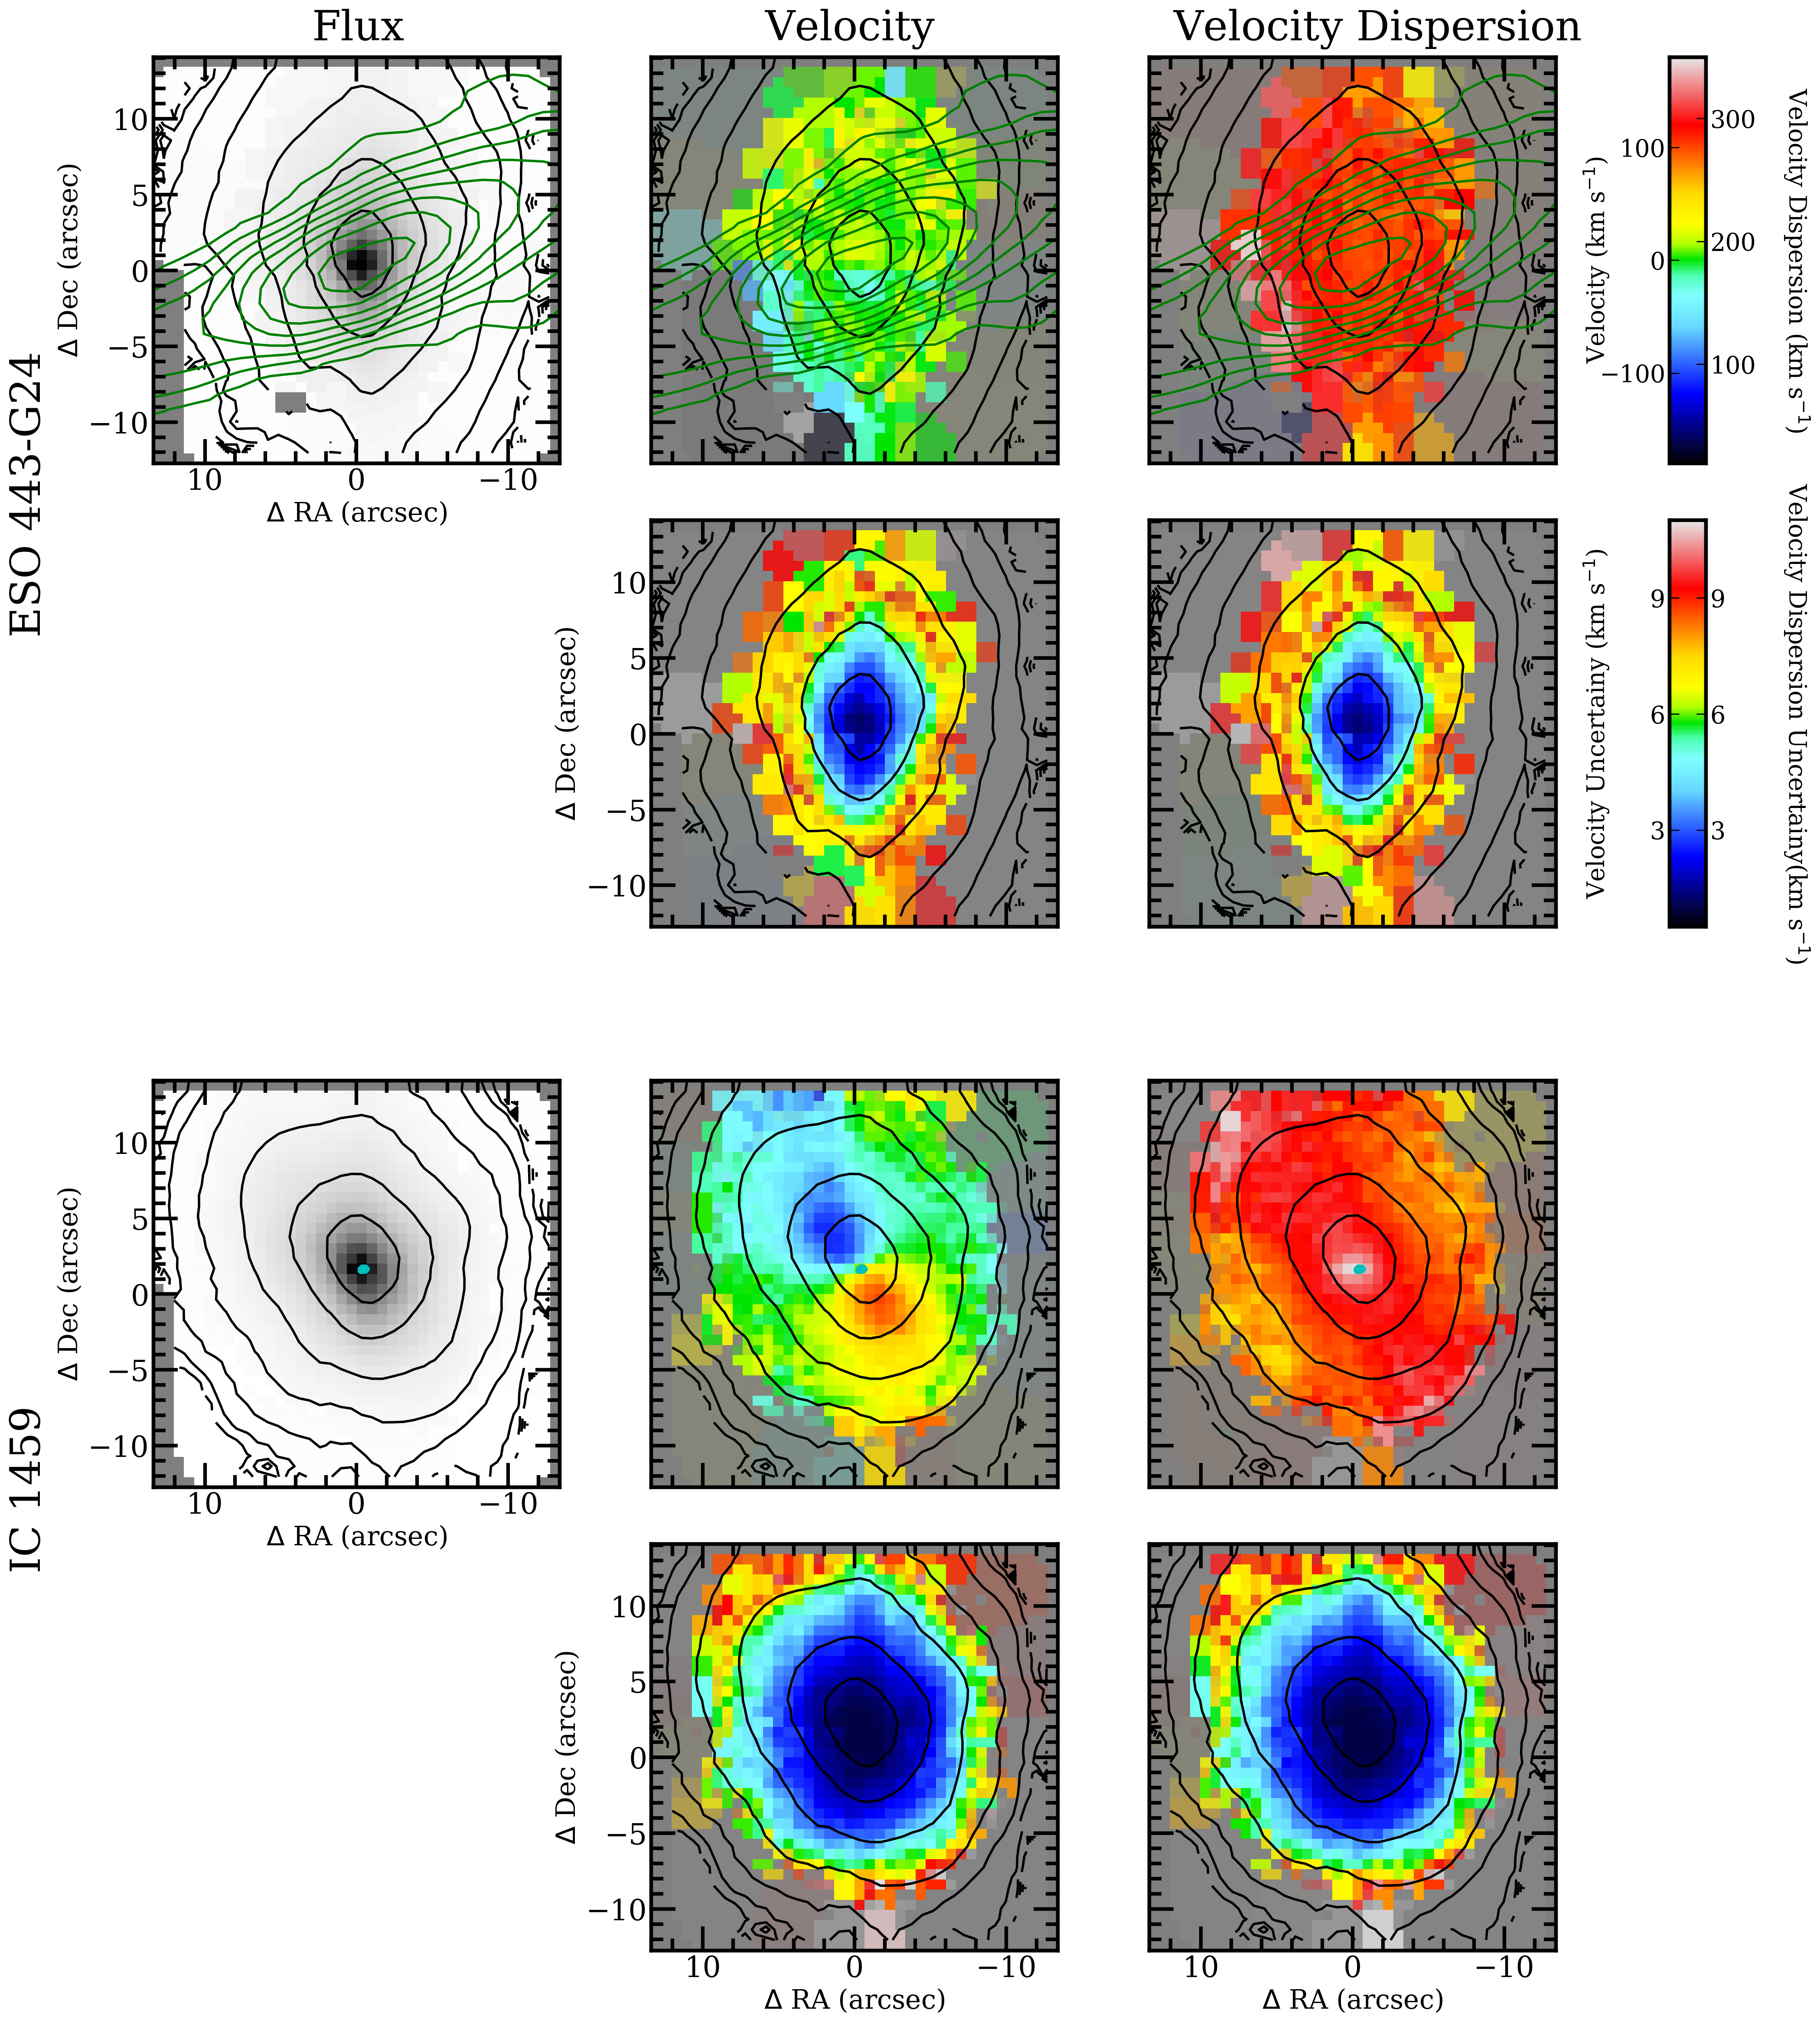
\includegraphics[height=0.62\textheight]{chapter4/vimos/kin1.png}
			\caption[VIMOS stellar kinematic maps]{VIMOS stellar kinematic maps: From left to right: flux (image), velocity and velocity dispersion. Top to bottom: ESO 443-G24 and IC 1459. Rows show parameter and uncertainty in the parameter on alternate rows. Flux contours are shown in black, CO from ALMA in cyan and radio from VLA in red. The radio band displayed depends on the data available in the archive and which images had a similar resolution and and scales. Limits on the color scale (min/max $\mathrm{km \, s^{-1}}$) are: velocity maps (-425/425), velocity uncertainty (1/19), velocity dispersion (30/36) and velocity dispersion uncertainty (1/33).} 
			\label{fig:VIMOS_stellar}
		\end{figure}
		\begin{figure}
			\centering
			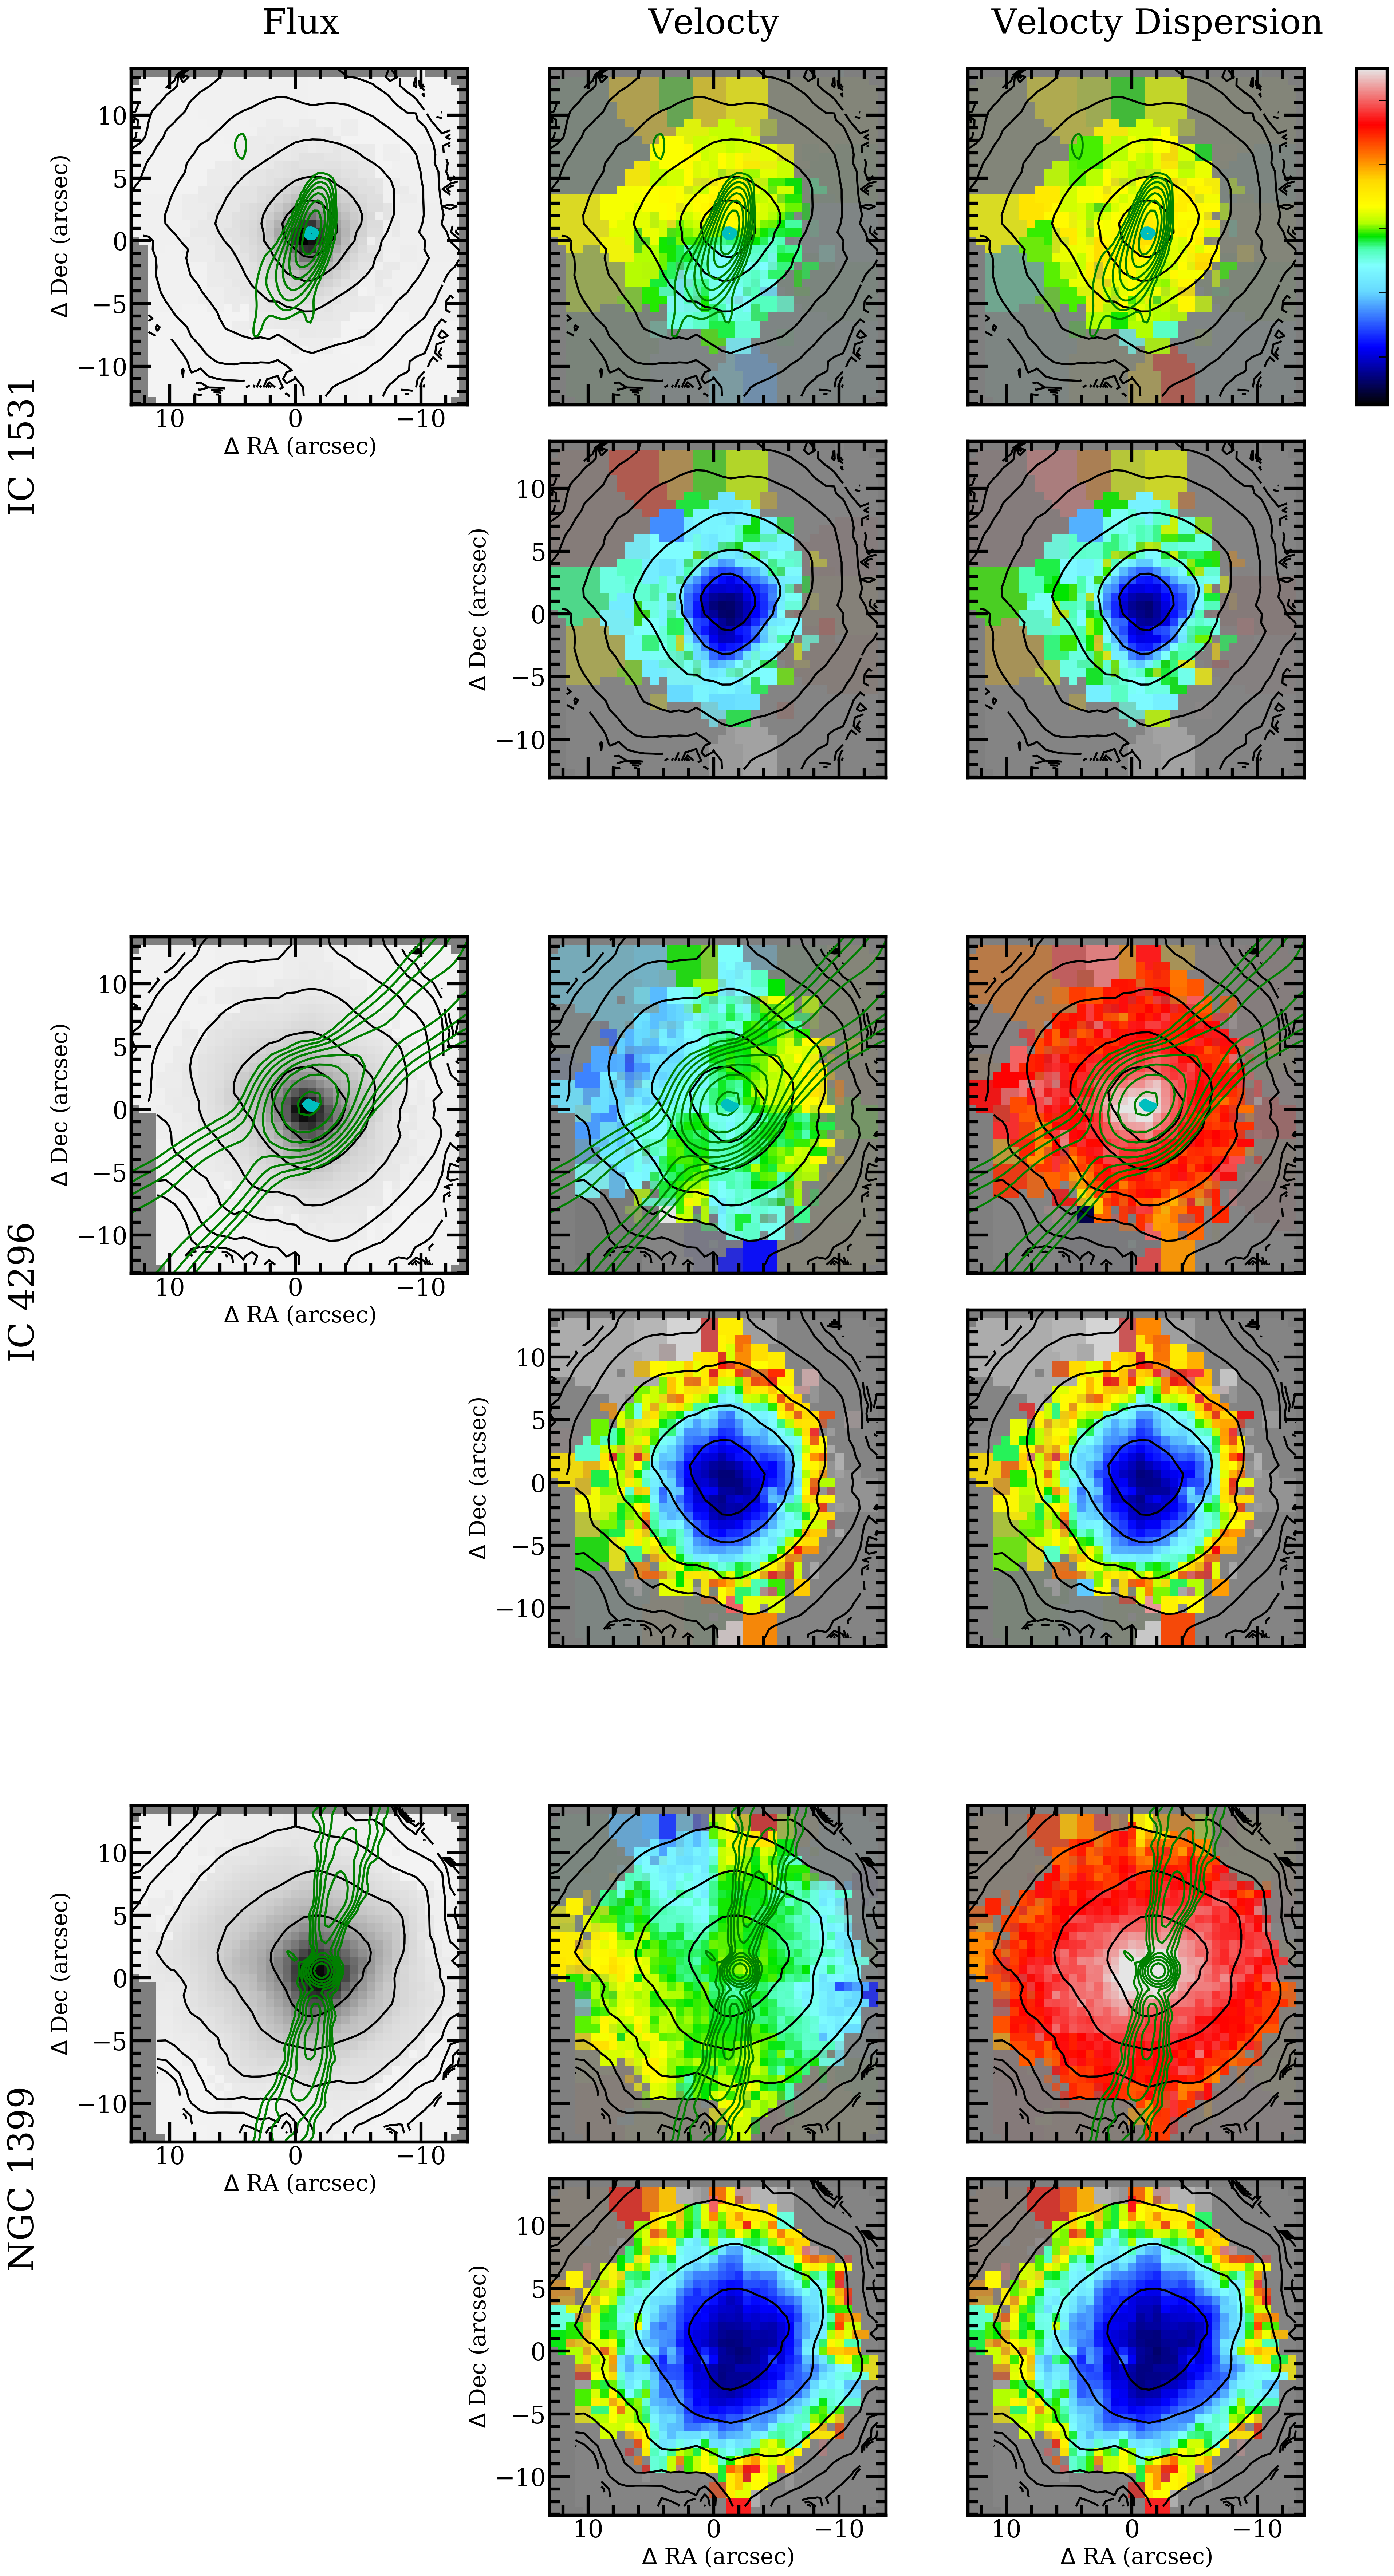
\includegraphics[height=0.94\textheight]{chapter4/vimos/kin2.png}
			\contcaption{continued for IC 1531, IC 4296 and NGC 1399.}
		\end{figure}
		\begin{figure}
			\centering
			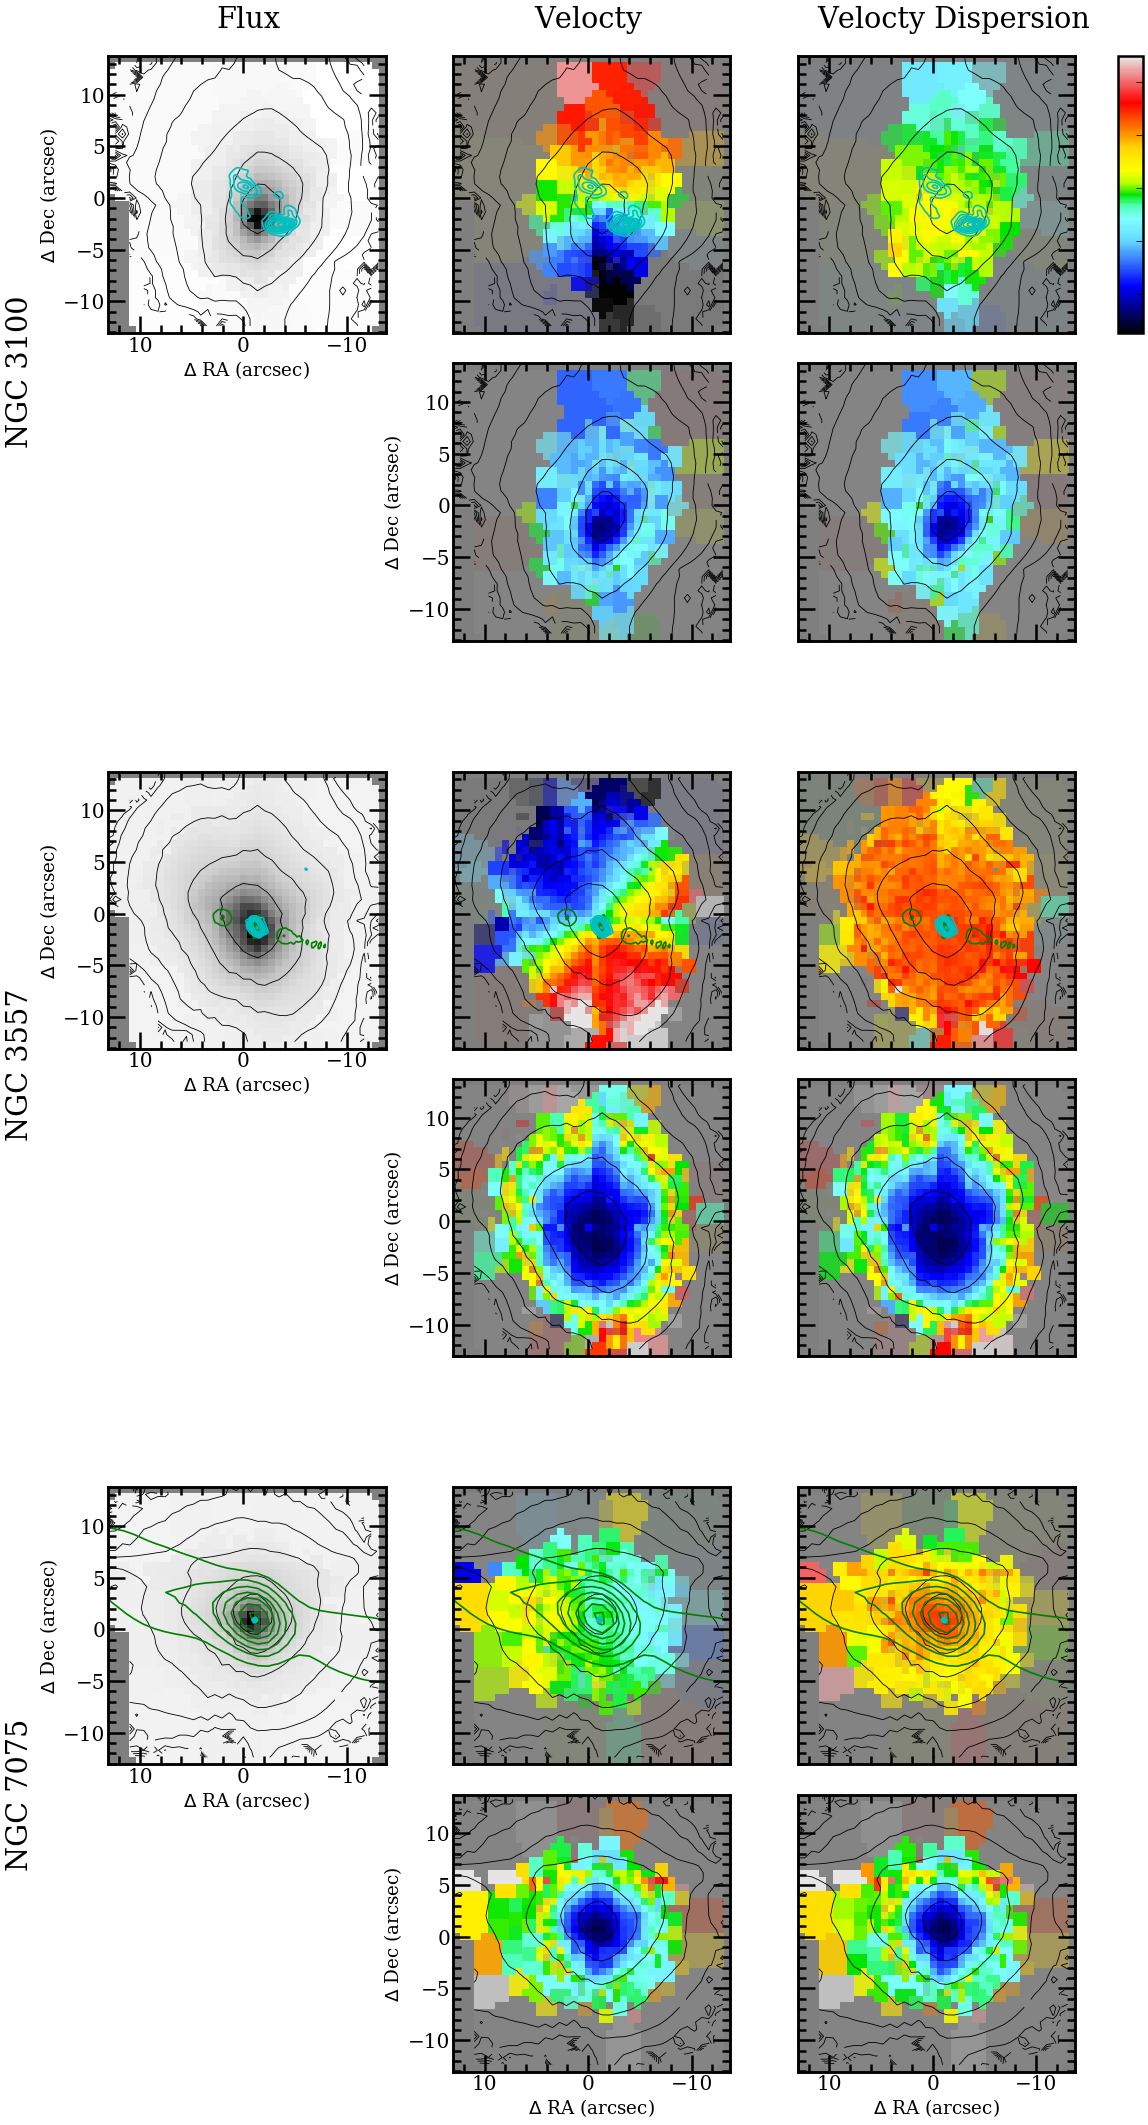
\includegraphics[height=0.94\textheight]{chapter4/vimos/kin3.png}
			\contcaption{continued for NGC3100, NGC 3557 and NGC 7075.}
		\end{figure}
		\begin{figure}
			\centering
			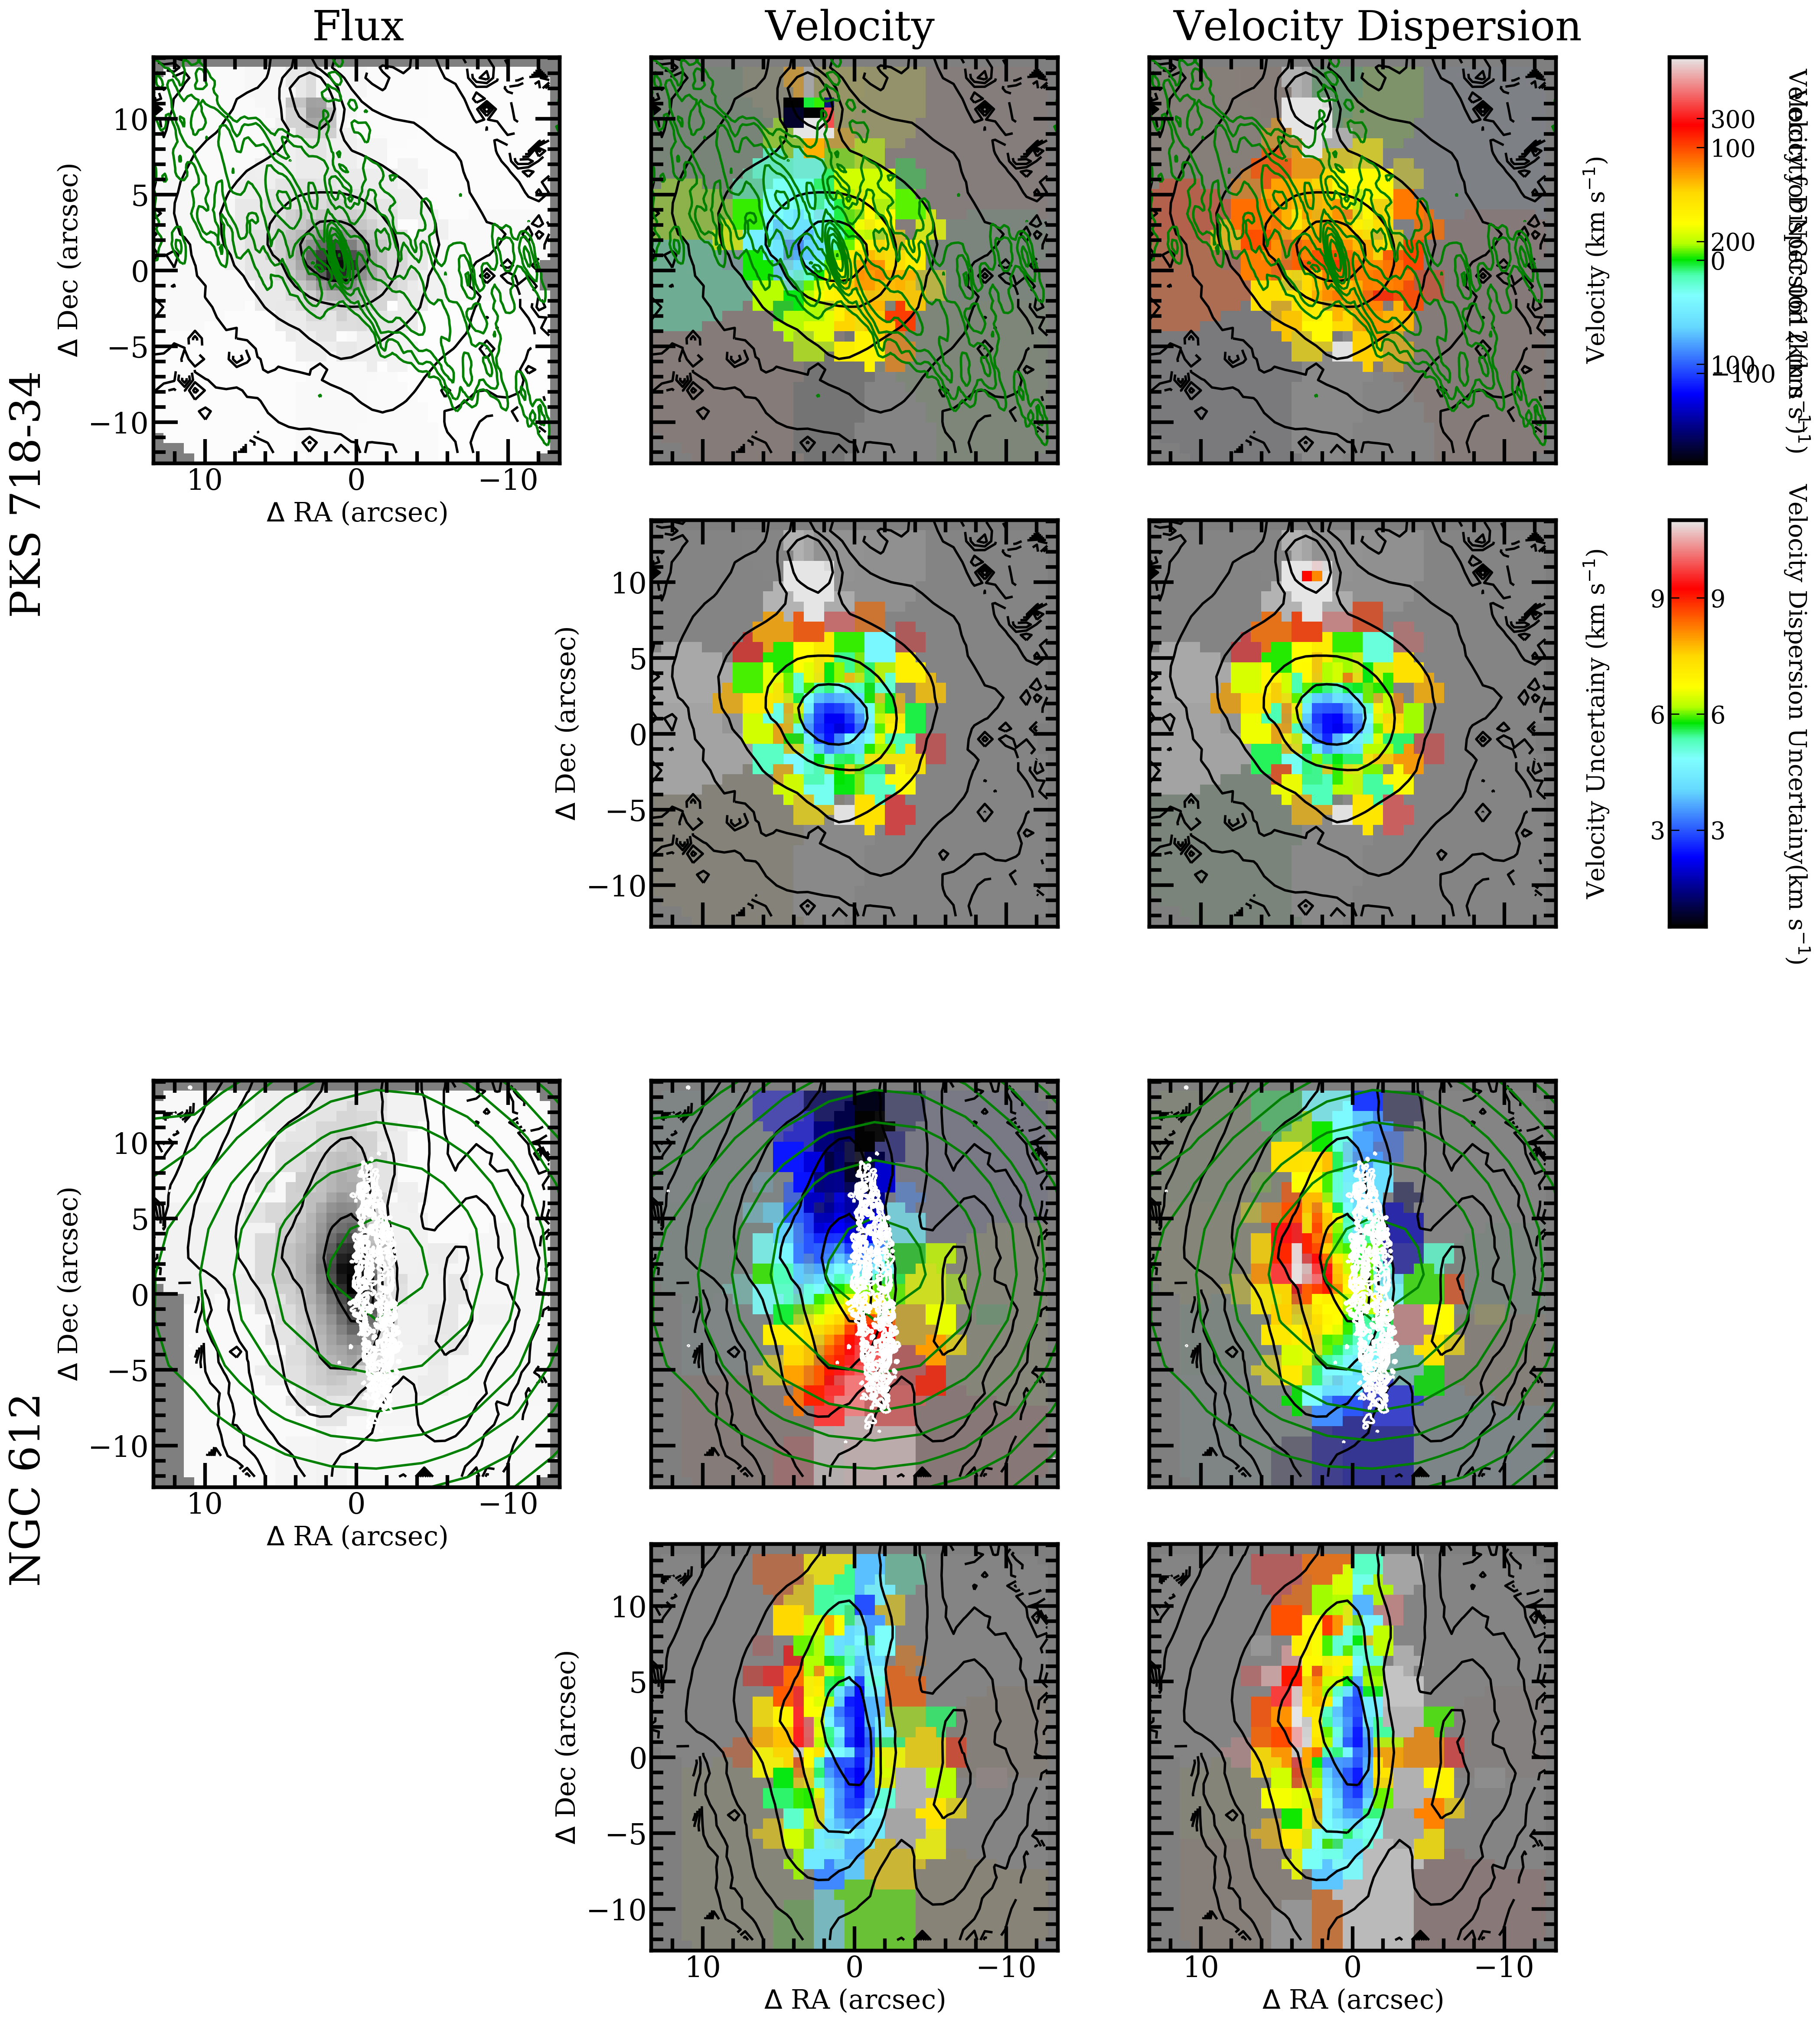
\includegraphics[height=0.62\textheight]{chapter4/vimos/kin4.png}
			\contcaption{continued for PKS 718-34 and NGC 612. The color scale for NGC 612 for the velocity map is from $-322 \, \mathrm{km \, s^{-1}}$ to $322 \, \mathrm{km \, s^{-1}}$.}
		\end{figure}

% Change NGC 1316 to 2nd figure in caption
		\begin{figure}
			\centering
			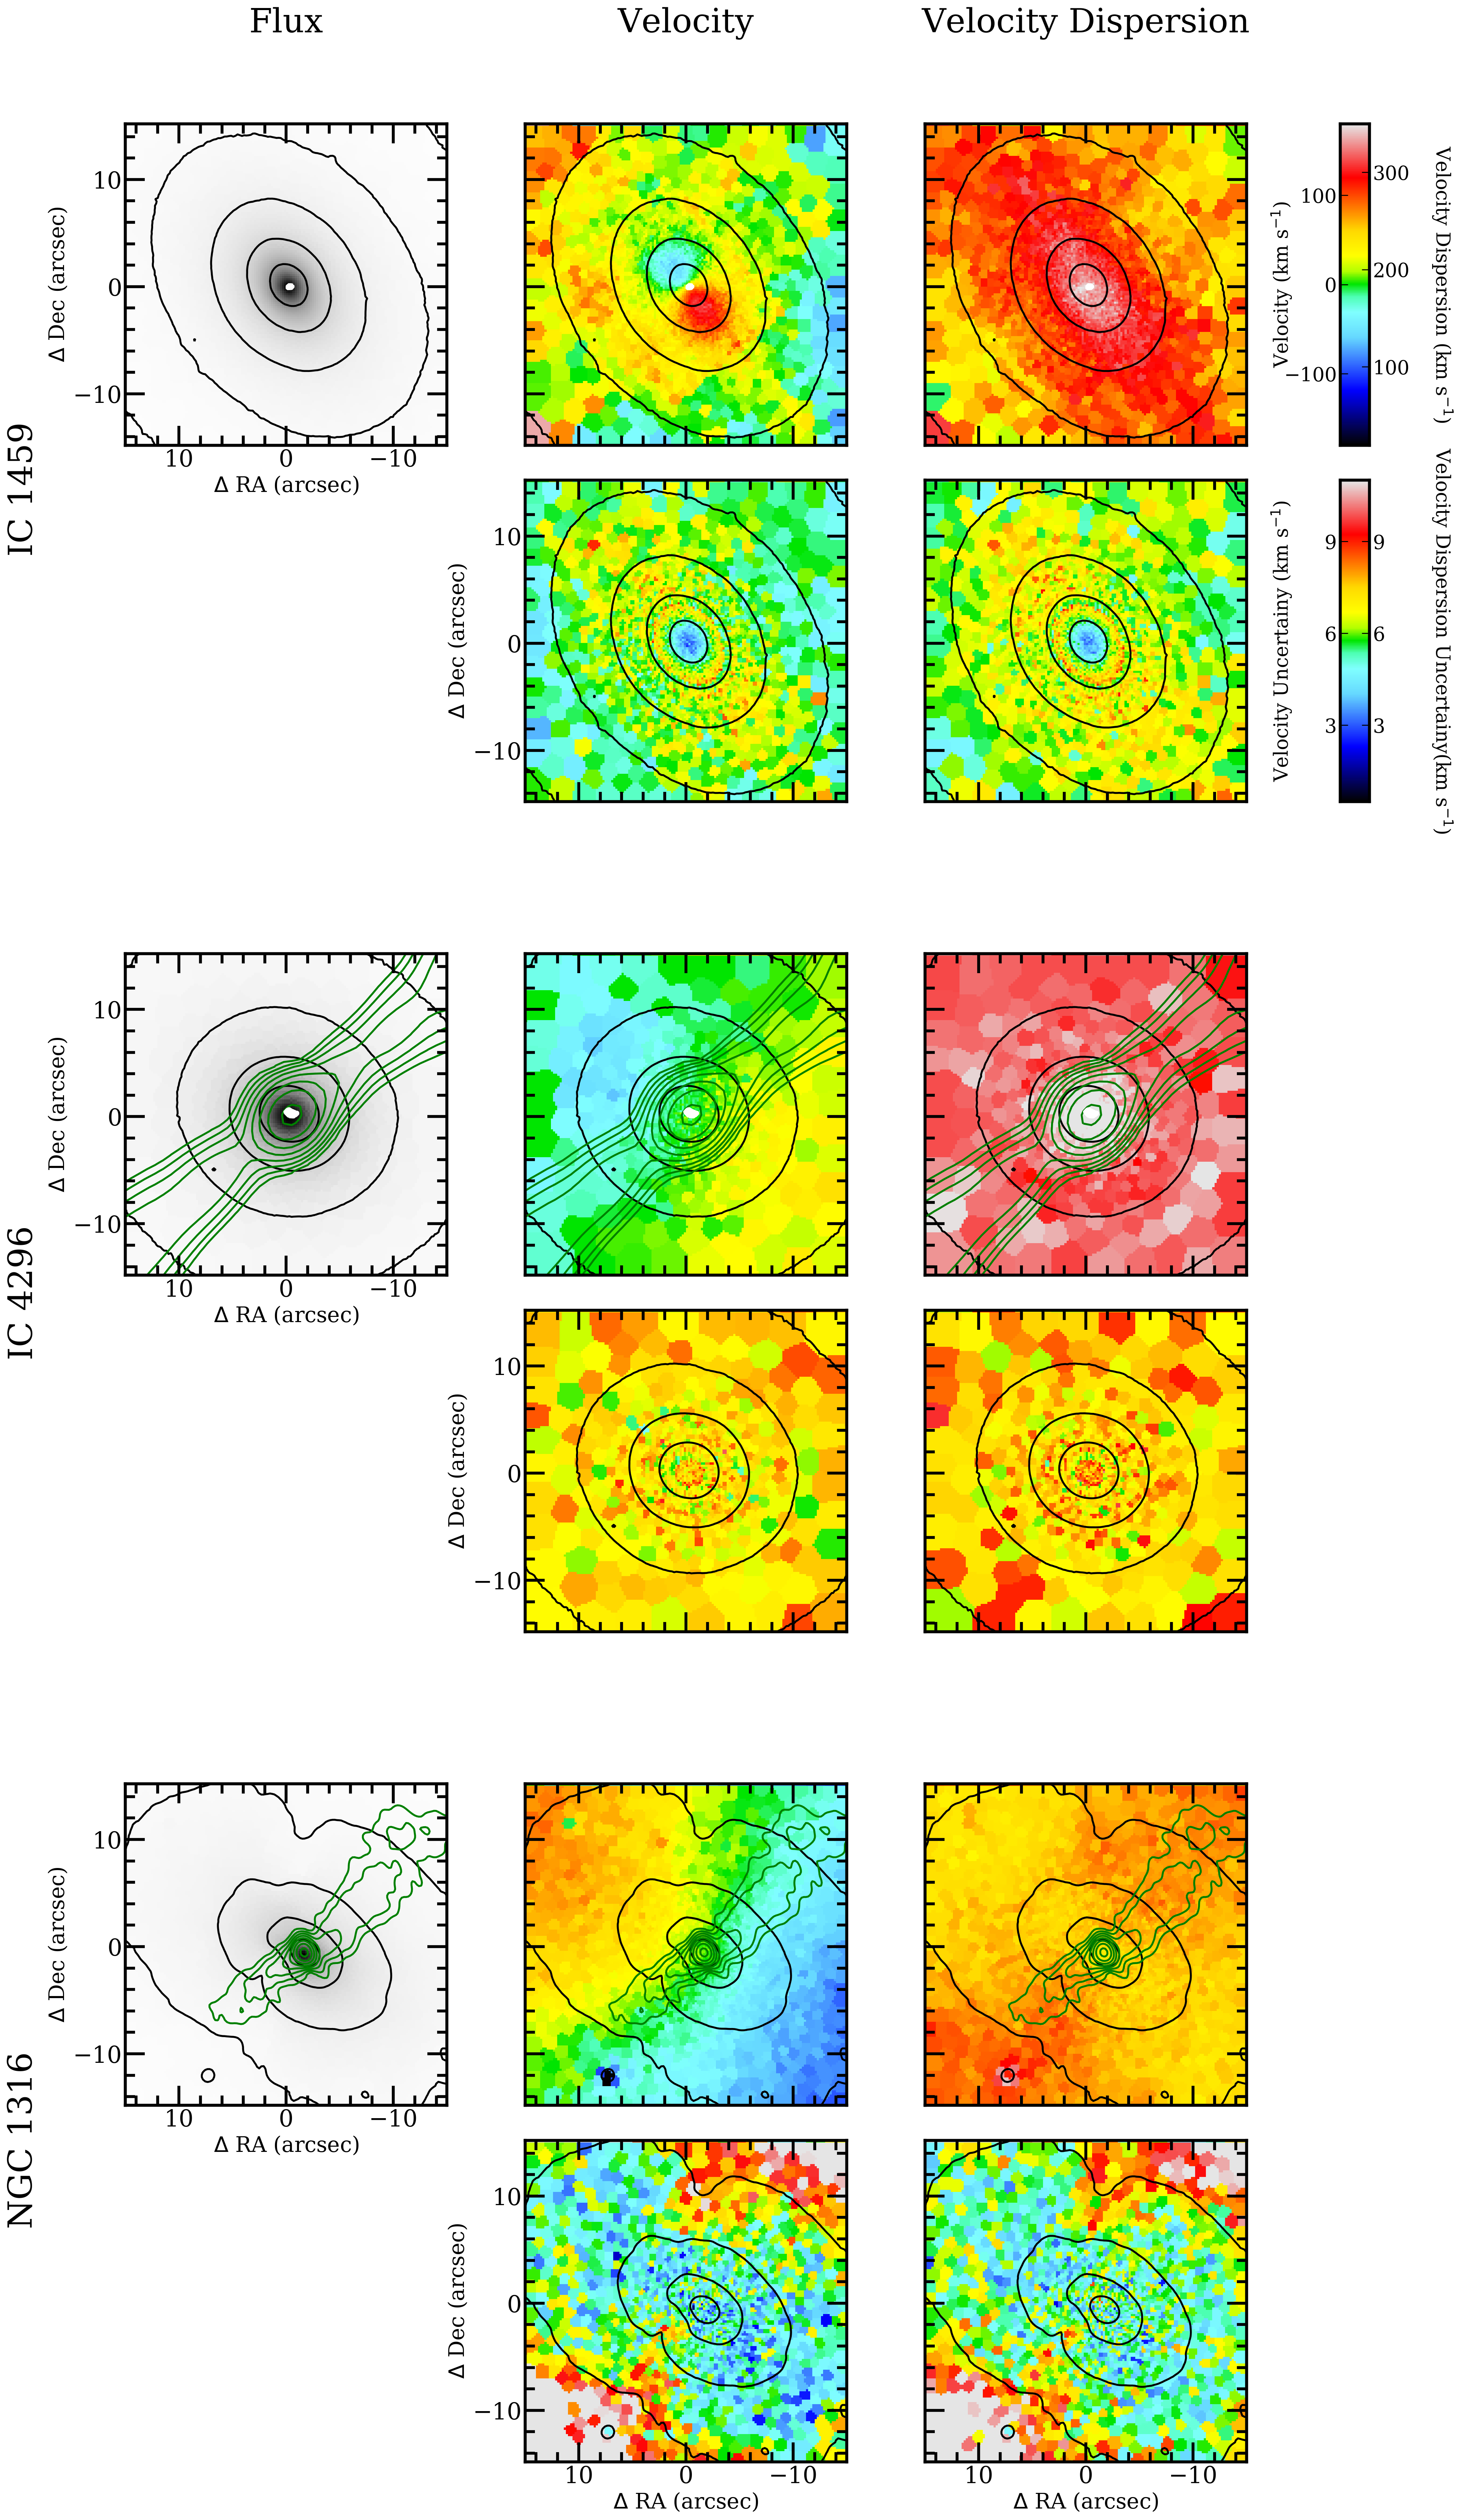
\includegraphics[height=0.94\textheight]{chapter4/muse/kin1.png}
			\caption[MUSE stellar kinematic maps]{MUSE stellar kinematic maps: From top to bottom: IC 1459, IC 4296 and NGC 1316. Plots are as in \ref{fig:MUSE_stellar} with the limits in the color scale (min/max $\mathrm{km \, s^{-1}}$): velocity maps (/), velocity uncertainty (/), velocity dispersion (/) and velocity dispersion uncertainty (/).}
			\label{fig:MUSE_stellar}
		\end{figure}
		\begin{figure}
			\centering
			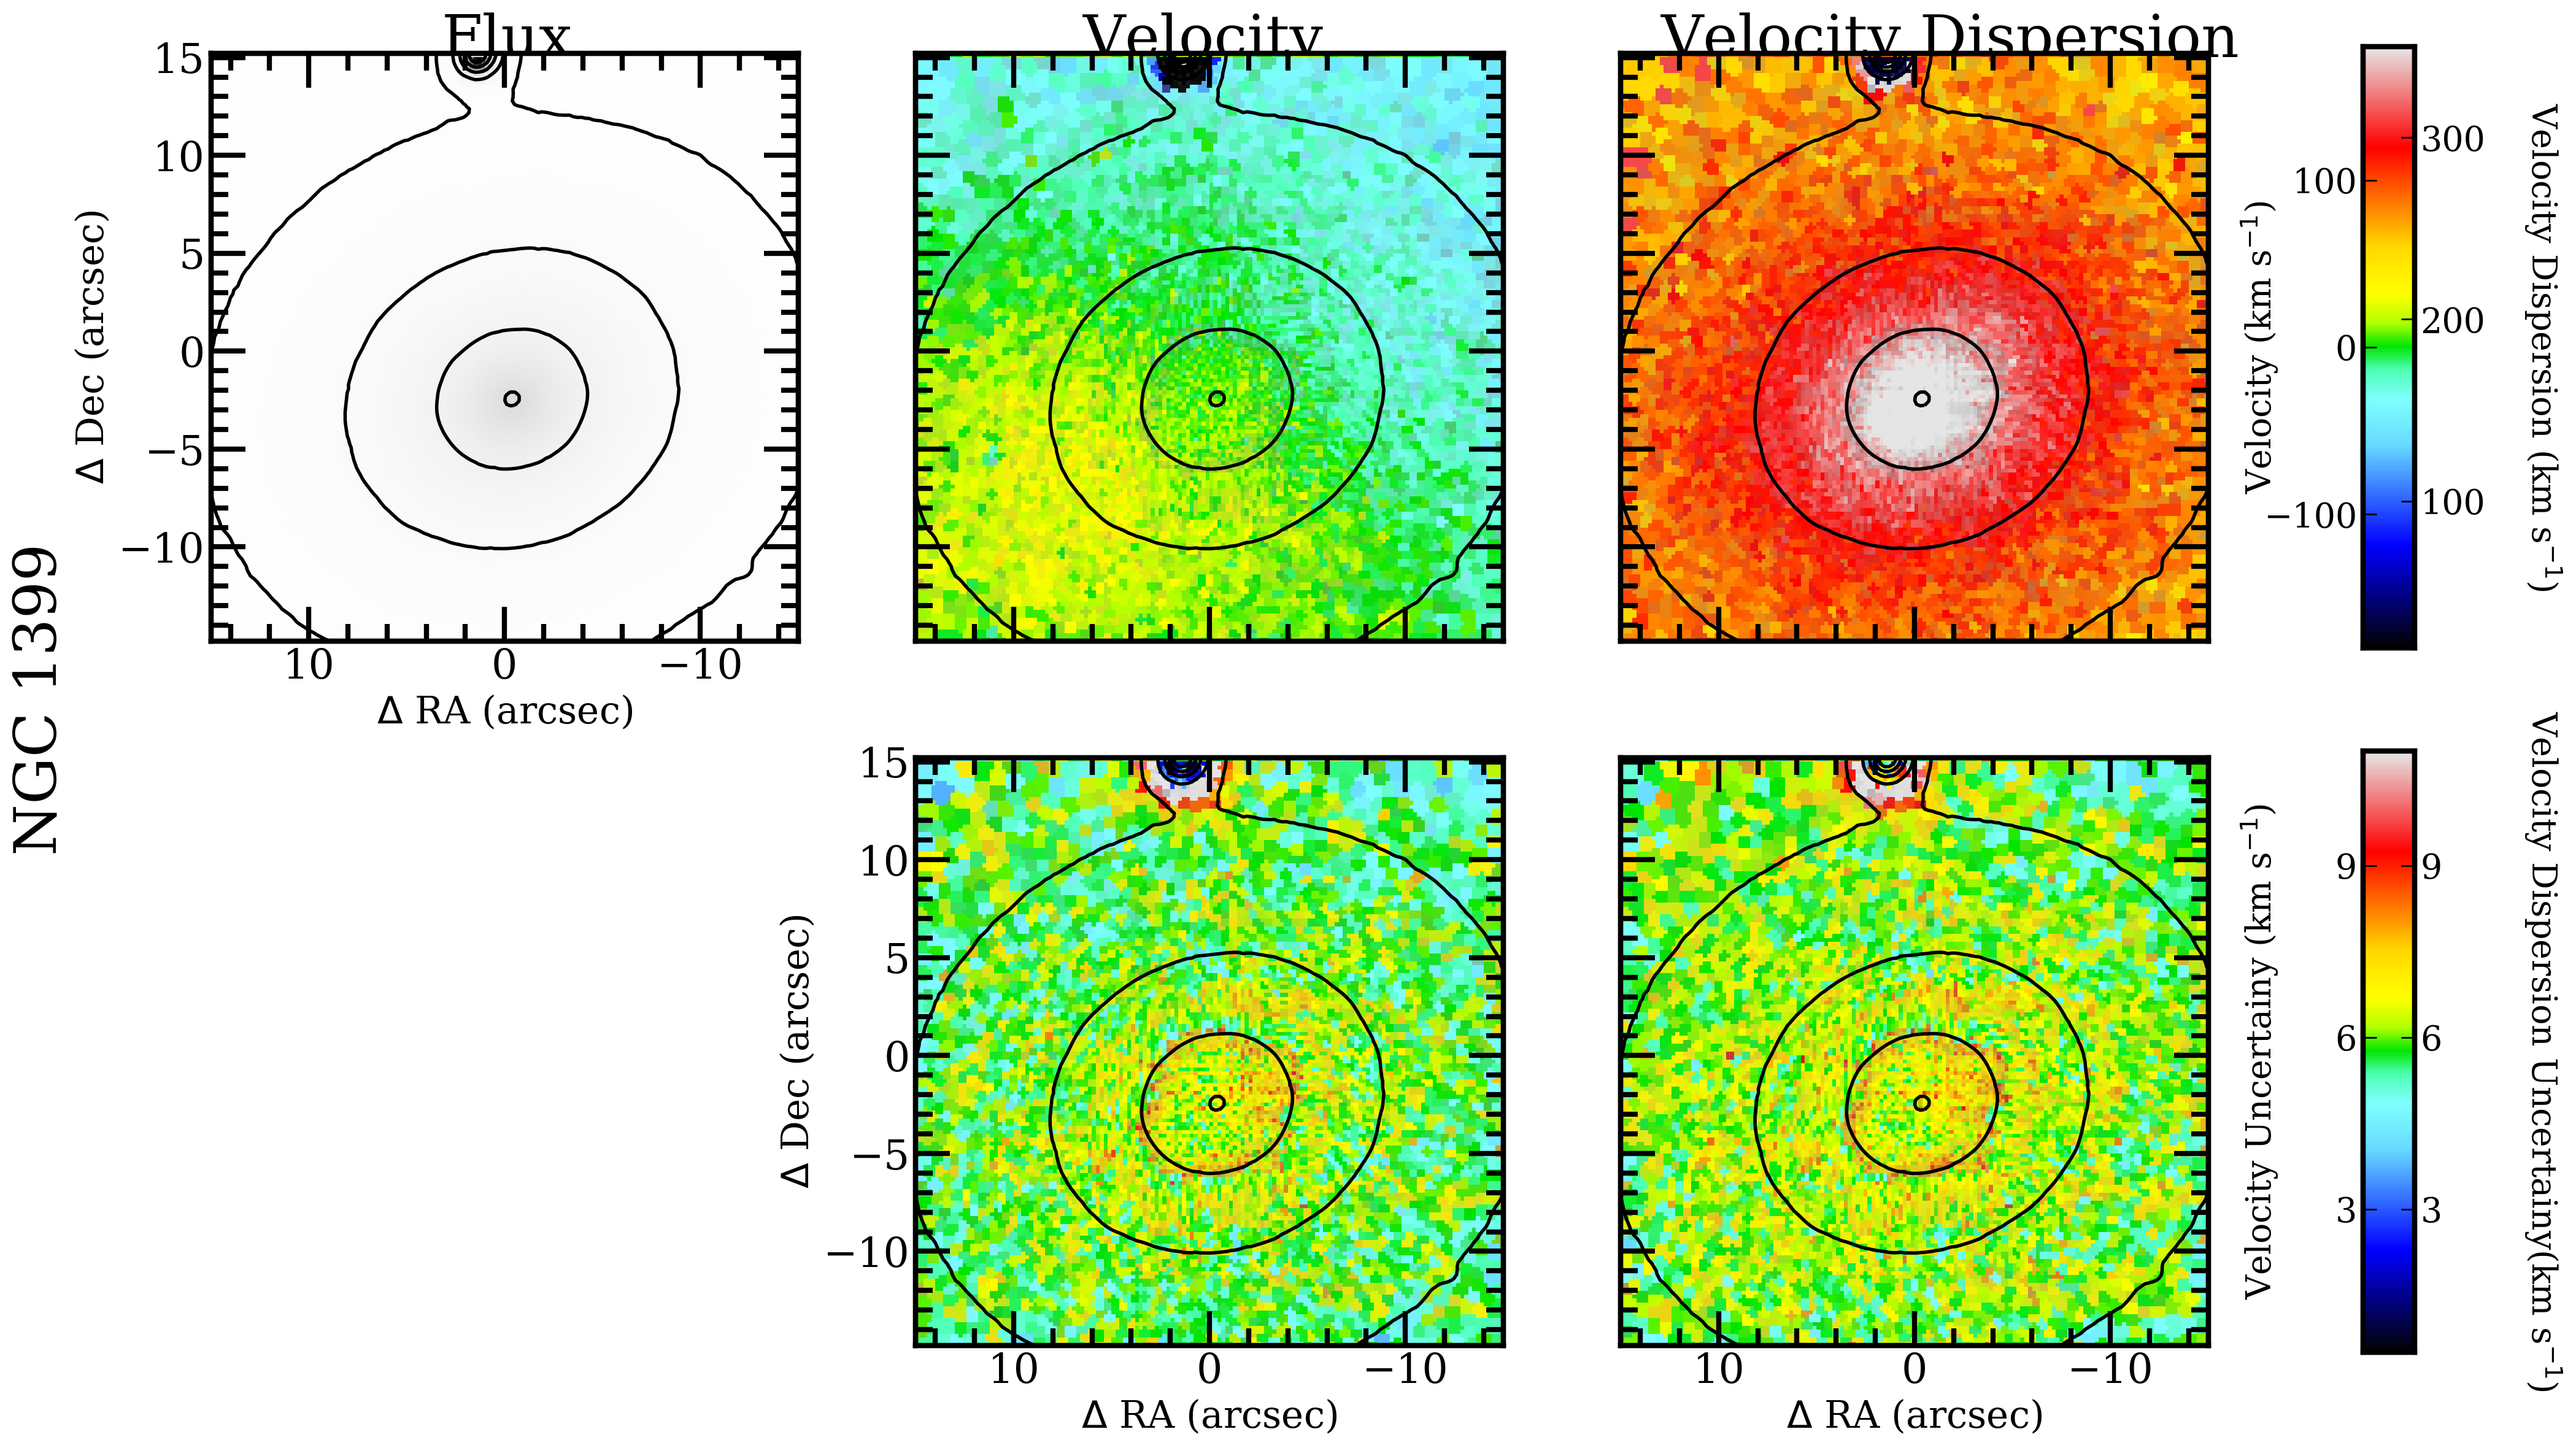
\includegraphics[height=0.31\textheight]{chapter4/muse/kin2.png}
			\contcaption{continued for NGC 1399}
		\end{figure}

		
		The kinematics of the sample are classified according to the regular-rotator/non regular-rotator (RR/NRR) regime given by \citet{Krajnovic2011} and fast/slow rotator (FR/SR) regime given by \citet{Cappellari2016} (originally defined by \citealt{Emsellem2011}, but later refined by \citealt{Cappellari2016}; see Section \ref{sec:ETG}). The $\lambda_{R_e}$--ellipticity plane is shown in figure \ref{fig:lambdaR_ellip}. Beyond this, we attempted to spot kinematic features, as defined in \citet{Krajnovic2011}, in an algorithmic way. However, artifacts from the VIMOS quadrants confuse any ellipse fitting methods and, as such, only maps from the MUSE data have been classified in this way: kinematic features in maps from VIMOS data were identified by eye. All these classifications are given in table \ref{tab:classify}. 


		\begin{table}
			\centering
		\begin{threeparttable}
			\caption{Kinematic classifications}
			\label{tab:classify}
			\begin{tabular}{l r r p{0.7cm} l l l l}
				\hline
				\hline
				Galaxy		& $\lambda_{R_e}$ & $\epsilon$  & $\Gamma_\text{kin}$ (deg) & FR/ SR 	& RR/ NRR 	& Feat. & Group 	\\
				\hline 
				ESO 443-G024 & 0.031 & 0.32 & 55.2 	& FR & NRR & KDC & c \\
				IC 1459 	& 0.174 & 0.24 & 87.9	& SR & NRR & KDC & c \\
				IC 1531 	& 0.100 & 0.11 & 64.4 	& SR & NRR & LV & a \\
				IC 4296		& 0.034 & 0.03 & 83.2 	& SR & RR & -- & e \\
				NGC 612 	& 0.519 & 0.58 & \leavevmode\phantom{0}7.3 	& FR & RR & -- & e \\
				NGC 1316 	& 0.100 & 0.39 & 72.1 	& FR & NRR & -- & f \\
				NGC 1399 	& 0.090 & 0.12 & 27.2 	& SR & NRR & LV & a \\
				NGC 3100 	& 0.418 & 0.31 & 19.8 	& FR & RR & -- & e \\
				NGC 3557 	& 0.320 & 0.22 & \leavevmode\phantom{0}7.6 	& FR & RR & -- & e\\
				NGC 7075 	& 0.048 & 0.09 & 20.0 	& SR & NRR & -- & b \\
				PKS 718-34  & 0.152 & 0.18 & 57.7 	& SR & NRR & KDC$^\text{a}$ & b\\
				\hline
				\hline
			\end{tabular}
			\begin{tablenotes}
			\small
			\item $^\text{a}$ This is a tentative classification. A higher signal to noise ratio (S/N) is required to a larger radii to confirm this.
			\item Here and hereafter where MUSE datacubes exist, their derived properties are quoted preferentially. Otherwise the values are VIMOS derived properties. 
			\item Col. 1: Galaxy name, Col. 2: $\lambda_\mathrm{R_e}$, Col. 3: Ellipticity, Col. 4: Misalignment between kinematic position angle and photometric position angle, Col. 5: Fast or slow rotator, Col. 6: Regular rotator or non-regular rotator, Col. 7: Kinematic features (abbreviations defined in section \ref{sec:ETG}), Col. 8: Kinematic group as defined in section \ref{sec:ETG}
			\end{tablenotes}
		\end{threeparttable}
		\end{table}

		The photometric position angle, $PA_\text{phot}$, is the angle of axis from North along which the surface brightness reaches the maximum values. Similarly, the kinematic position angle, $PA_\text{kin}$, is the angle of axis from North along which the projected velocities reaches the maximum absolute values. Column 4 in table \ref{tab:classify} shows the misalignment between the photometric position angle and the kinematic position angle, $\Gamma_\text{kin} = \left| PA_\text{phot} - PA_\text{kin} \right|$. \citet{Cappellari2007}, \citet{Krajnovic2011} and \citet{Fogarty2015} all show that regular rotating galaxies (hereafter referred to as regular rotators) almost always have aligned kinematic and photometric axes (with a scatter of 4$\degree$). 
		Regular rotators with a significant misalignment are either very round, interacting or strongly barred (see figure \ref{fig:Misalignment}). Taking into account the lower quality of data, our results are consistent with this. Of the 4 regularly rotating galaxies in the Southern sample, 2 are misaligned to less than 8$\degree$ (NGC 612 and NGC 3557) and the other 2 are round ($\epsilon < 0.3$; IC 4296 and NGC 3100). As noted in \citet{Cappellari2016}, this result requires that regular rotators are axis-symmetric.

		Misalignments between the photometric and kinematic position angles are routinely observed for non-regularly rotating galaxies (hereafter referred to as non regular-rotators). This generally implies a more triaxial intrinsic shape, however large misalignments are extremely rarely observed in galaxies with $\epsilon > 0.4$. This suggests that non-regularly rotating galaxies are more spherical in shape. This is the reason for the $\epsilon < 0.4$ requirement in the definition for slow rotators. The non-regular rotators in our sample all have $\epsilon < 0.4$. 


	\subsection{Fast/Slow Rotator Fraction}
		\label{subsec:FSfrac}
		The radial $\lambda_{R_e}$ profiles are shown in figure \ref{fig:lambdaR_profile}. Using the combined samples from Atlas$^\text{3D}$ and MASSIVE (hereafter the combined sample), we find that there is no discernible difference between the radio selected Southern Sample and the optically selected ETGs, once the difference in mass distribution is taken into account. 
		We find the expected fraction of slow rotators in the southern sample, $f'$, corrected to the mass distribution of the combined sample as
		\begin{equation}
			f' = \sum_{n=0}^N N_\mathrm{SS} f_\mathrm{CS}\, , 
		\end{equation}
		where $N_\mathrm{SS}$ is the number of southern sample galaxies in the n$^\mathrm{th}$ mass bin, $N_\mathrm{CS}$ is the fraction of slow rotators in the n$^\mathrm{th}$ in the combined sample and $N$ is the total number of mass bins. In our case we use K-band magnitude ($M_K$) as a proxy for mass, with bins 0.5 mag wide. This gives $f' = 0.64 \pm 0.06$. This is consistent with our finding of 56\% of the Southern Sample being slow rotators.

		\begin{figure}
			\centering
			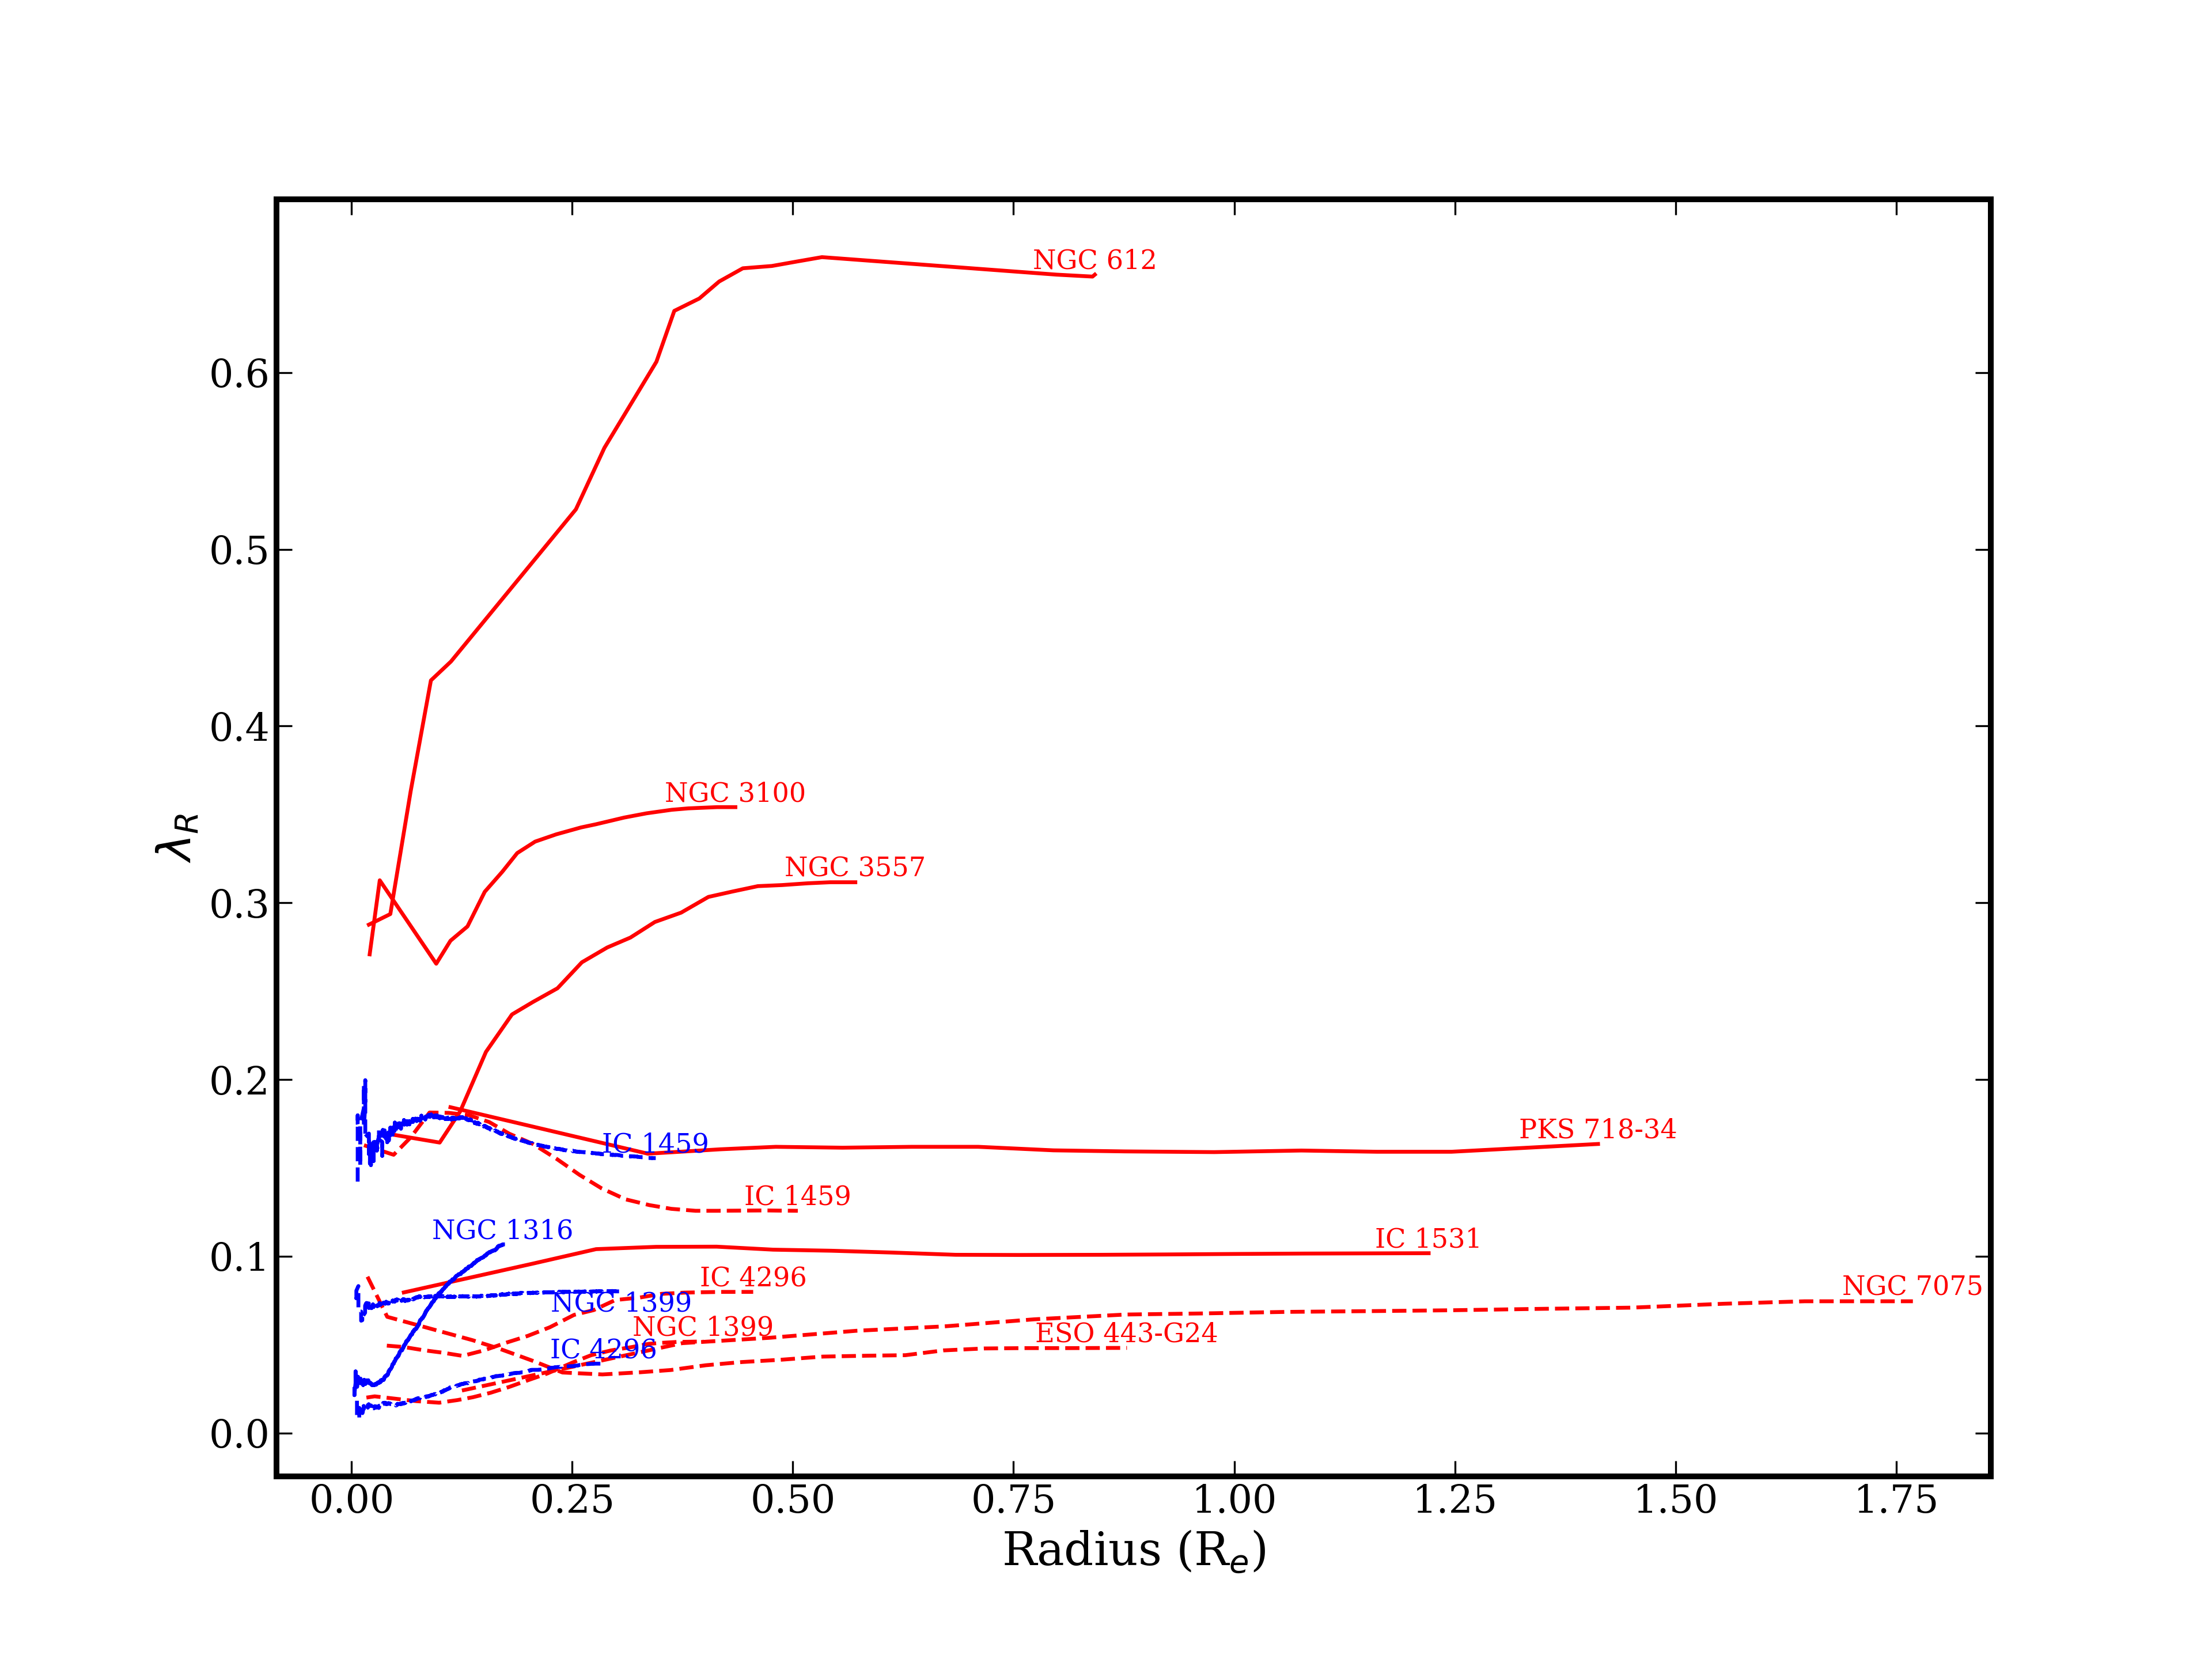
\includegraphics[width=.7\textwidth]{chapter4/lambda_R.png}
			\caption[$\lambda_{R}$ radial profiles]{The radial $\lambda_{R}$ profiles. Profiles from VIMOS data are in blue, while MUSE data is in red. Solid lines represent fast rotators, while dashed lines represent slow rotators.}
			\label{fig:lambdaR_profile}
		\end{figure}


		\begin{figure}
			\centering
			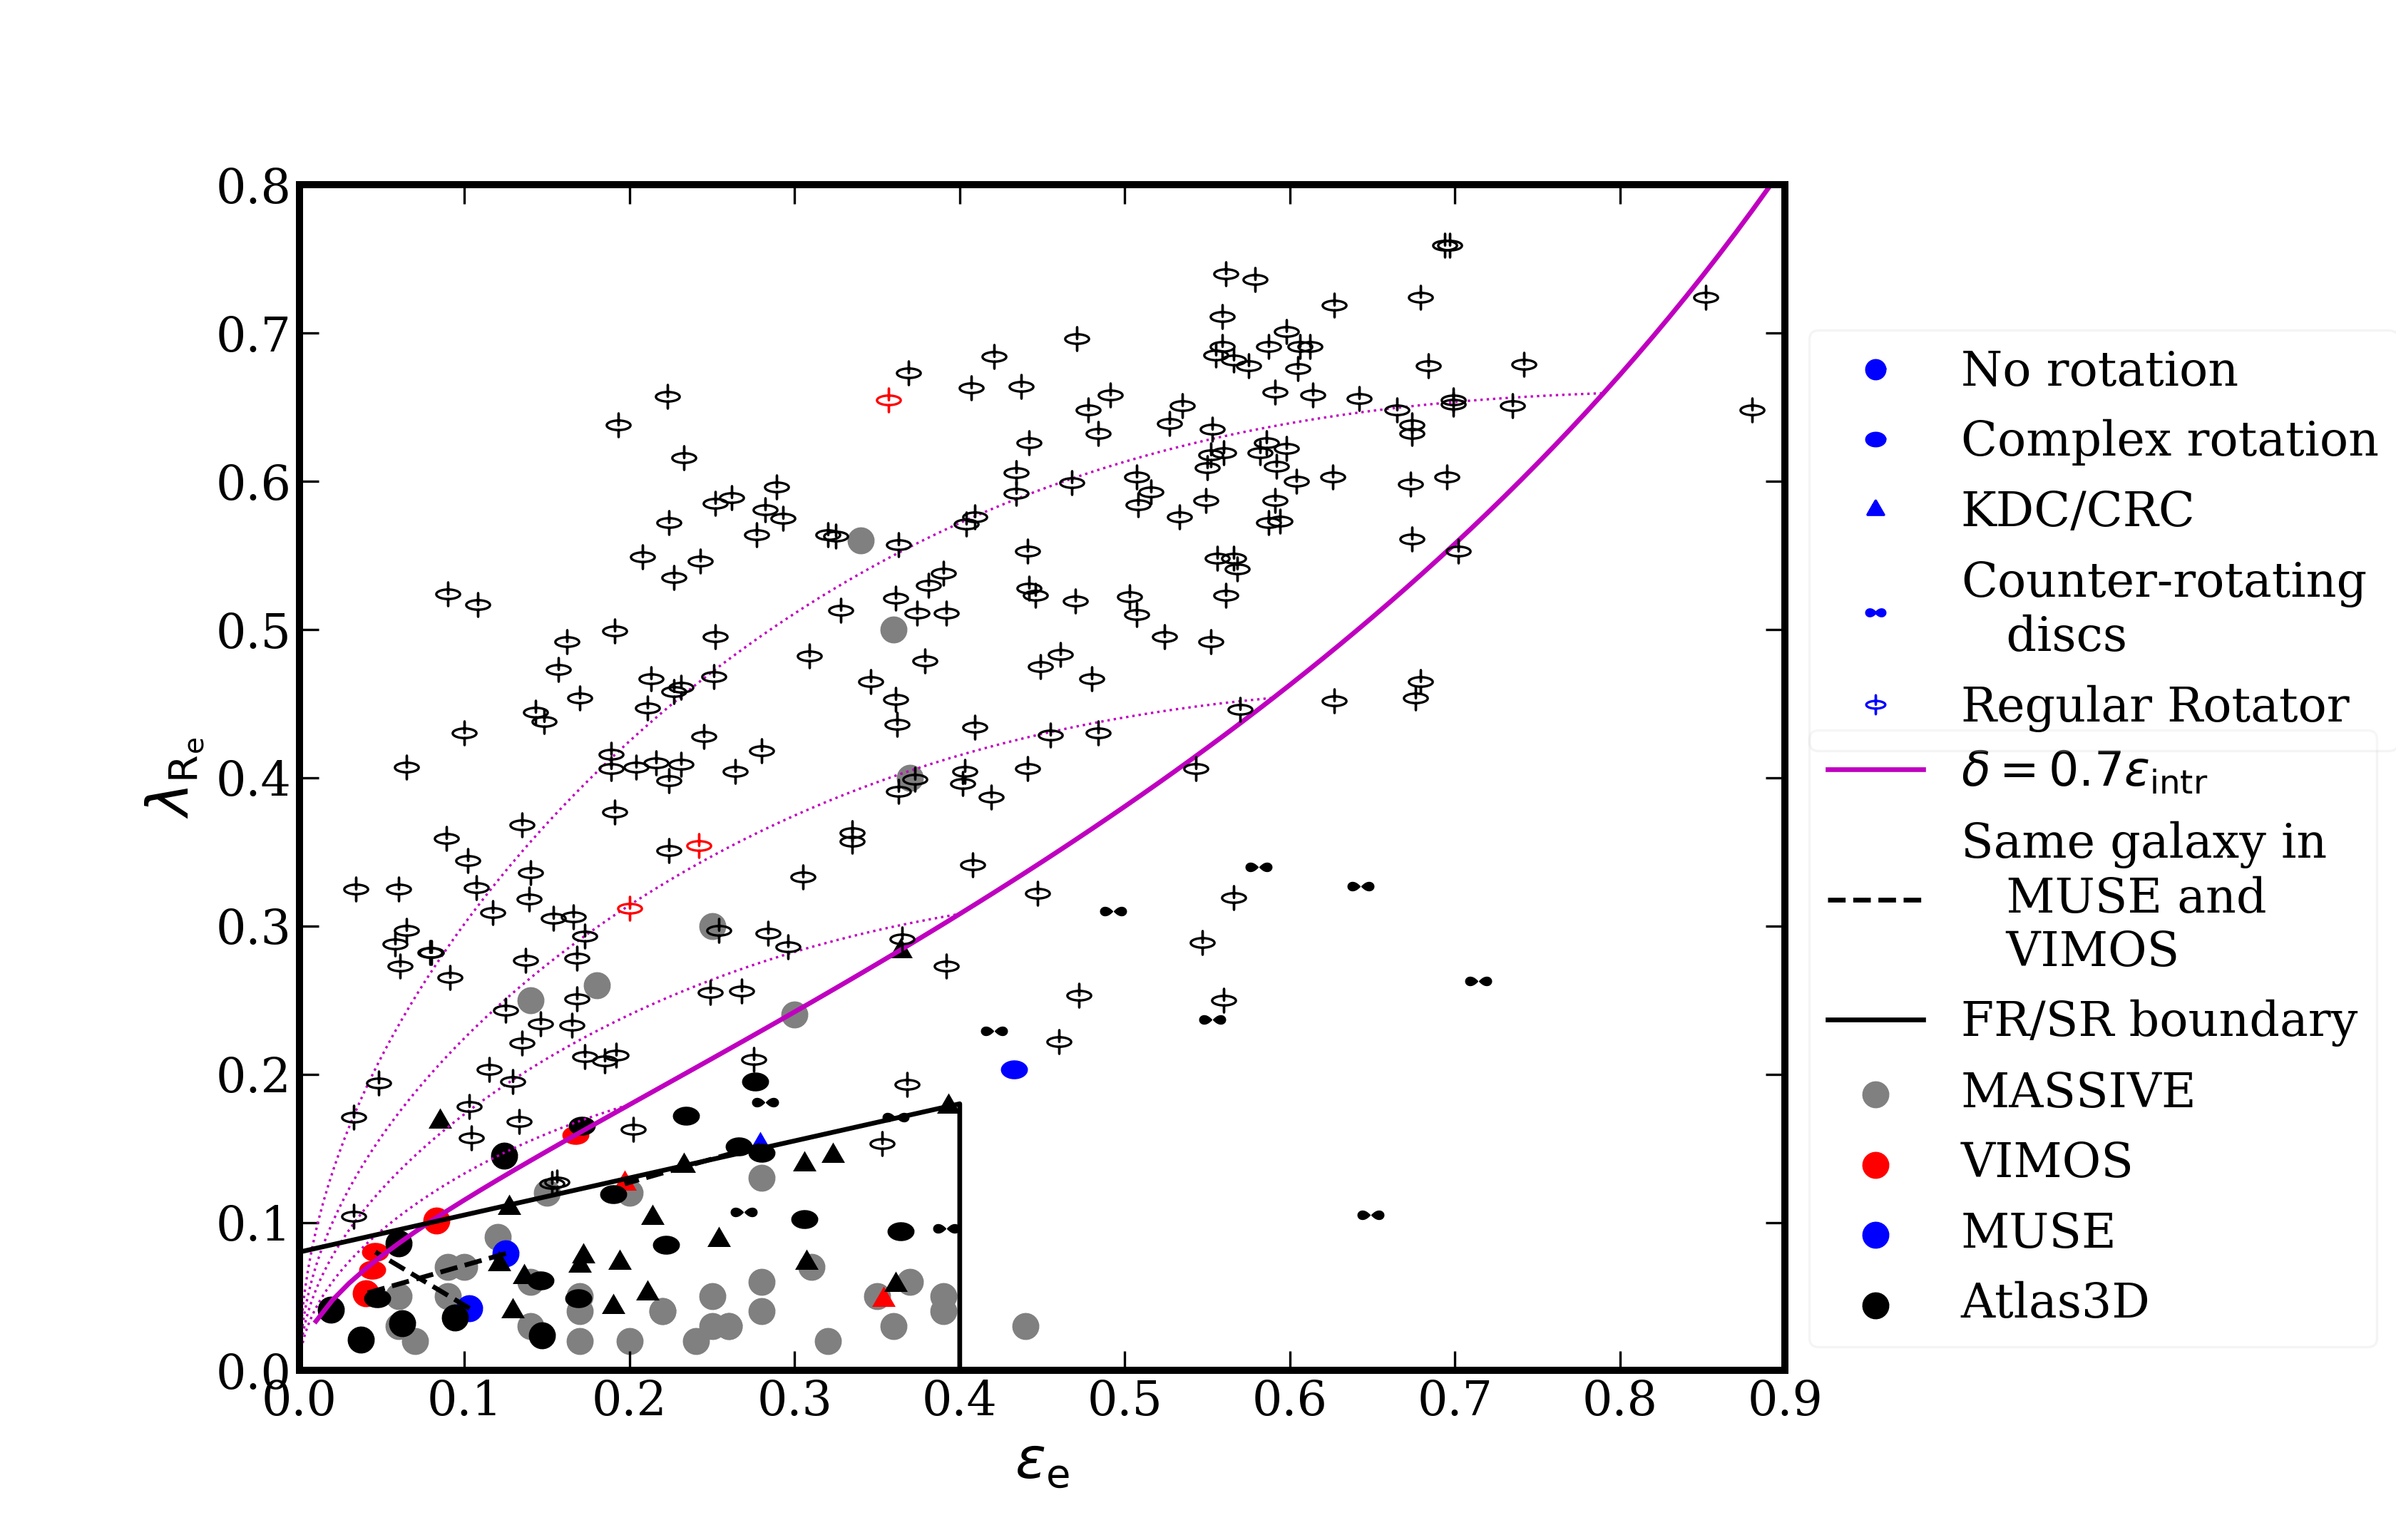
\includegraphics[width=0.7\textwidth]{chapter4/lambda_R_ellipticity.png}
			\caption[$\lambda_{R_e}$ -- ellipticity plane]{The $\lambda_{R_e}$ -- ellipticity plane showing the definition for the fast/slow rotator classes (solid black line). Atlas$^\text{3D}$ galaxies are shown in black \citep{Emsellem2011} and MASSIVE survey galaxies are shown in gray \citep{Veale2017}. VIMOS and MUSE measurements are shown in red and blue respectively. The theoretical limit of disc dominated galaxy is shown (solid magenta) with lines of constant intrinsic angular moment with varying inclination (dashed magenta). The MASSIVE survey does not classify substructure so the MASSIVE sample is simply shown with filled circles.}
			\label{fig:lambdaR_ellip}
		\end{figure}


		

		\begin{figure}
			\centering
			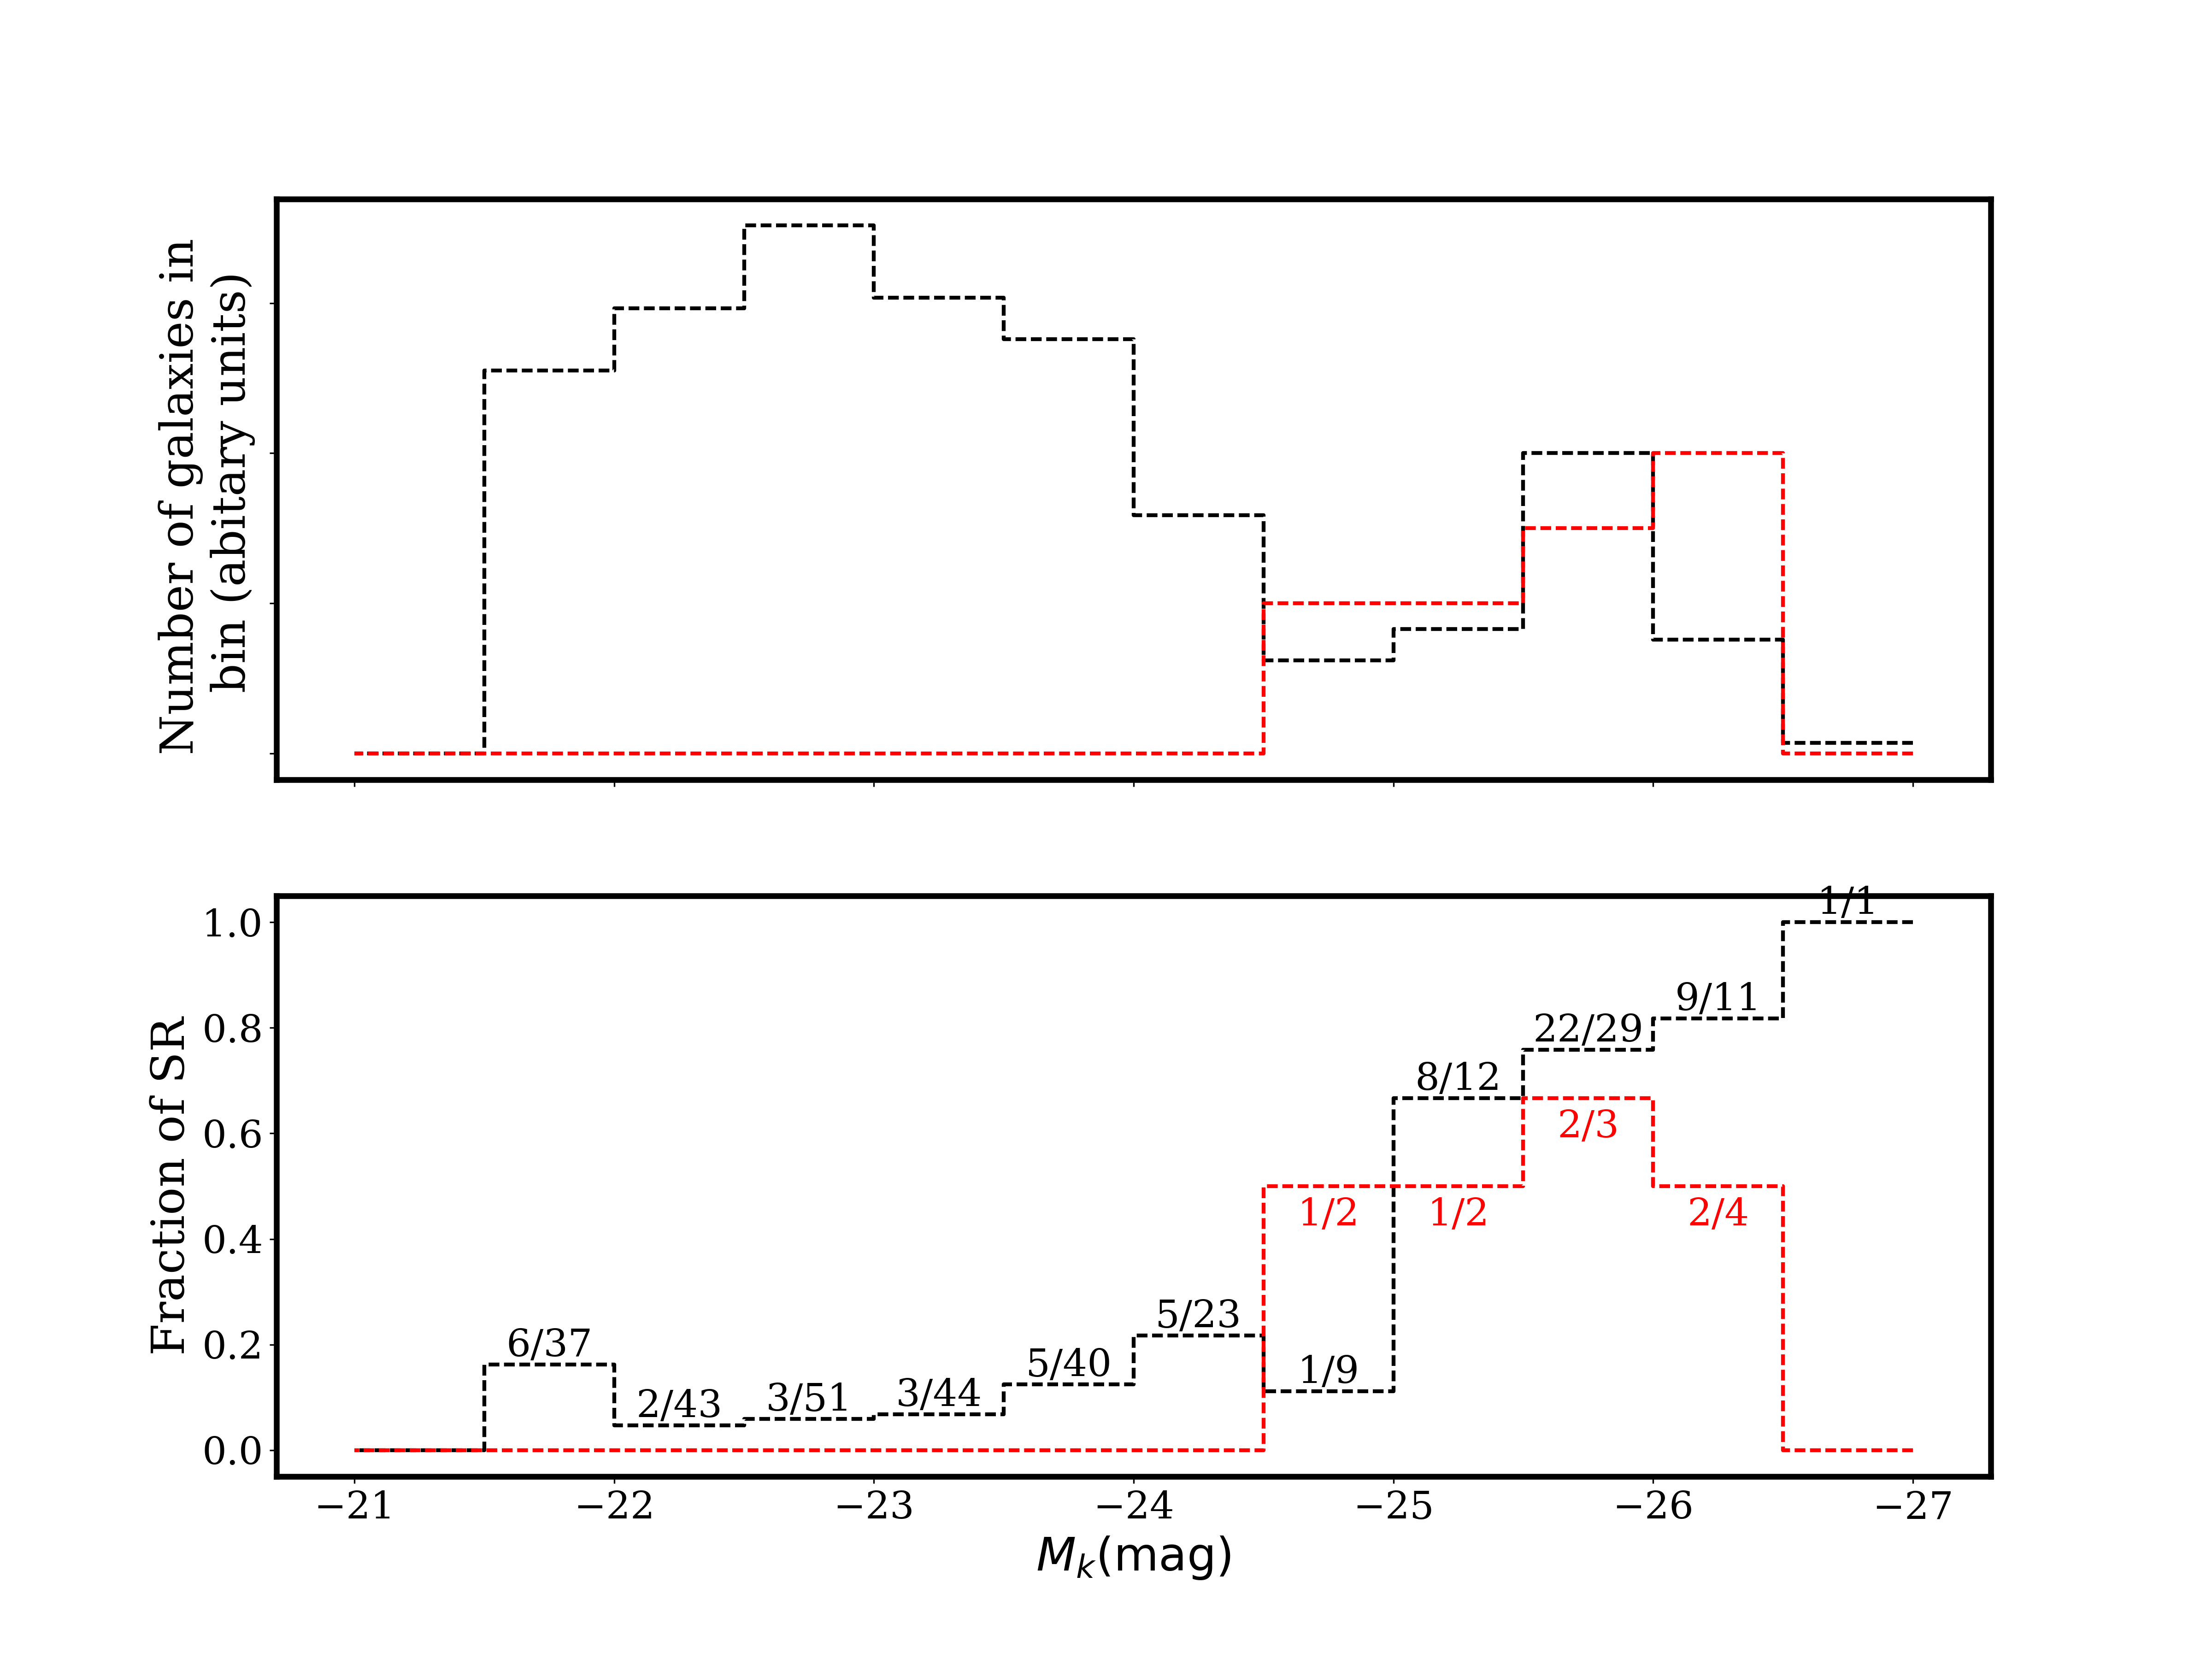
\includegraphics[width=0.8\textwidth]{chapter4/M_k_binned.png}
			\caption[Upper panel: Mass matching global kinematics]{The mass distributions of the combined Atlas$^\text{3D}$ and MASSIVE surveys (black) and the Southern Sample (red). Lower panel: the fraction of slow rotators within each mass bin. The labels display the [number of slow rotators]/[total number of galaxies] in that bin. Note that the black and red have different normalizations in the mass distribution plot: the combined Atlas$^\text{3D}$ and MASSIVE samples contains 300 galaxies, while the Southern Sample is just 11 radio galaxies.}
			\label{fig:SRmassFraction}
		\end{figure}


		


 


\section{Stellar Population}
	\label{sec:pop}

	\subsection{Absorption line strengths}
		\label{subsec:absorption}
		Figures \ref{fig:VIMOS_absorption} and \ref{fig:MUSE_absorption} show the resolved absorption line strengths for the Southern Sample. For the VIMOS datacubes, we find G4300, Fe4383, Ca4455, Fe4531, H$_\beta$, Fe5015 and Mg$_b$ indices (bandpasses are defined in table \ref{tab:abIndex}). For the most distant galaxies, the red continuum band for Mg$_b$ is redshifted beyond the range of the VIMOS spectrograph. In these cases we have not attempted to adjust the definition of the bandpass, but have simply not included Mg$_b$ in any future analysis. For MUSE datacubes, we find the H$_\beta$, Fe5015, Mg$_b$, Fe5270, Fe5335, Fe5406, Fe5709, Fe5782, NaD, TiO1 and TiO2 indices. 

		\begin{table}
			\centering
		\begin{threeparttable}
			\caption{Definitions of bandpasses for line indices.}
			\label{tab:abIndex}
			\begin{tabular}{l c c c}
				\hline
				\hline
				Index 	& Blue cont. 		& Index band 		& Red cont. \\
				\hline 
				G4300 	& 4266.375--4282.625 & 4281.375--4316.375 & 4318.875--4335.125 \\
				Fe4383 	& 4359.125--4370.375 & 4369.125--4420.375 & 4442.875--4455.375 \\
				Ca4455 	& 4445.875--4454.625 & 4452.125--4474.625 & 4477.125--4492.125 \\
				Fe4531 	& 4504.250--4514.250 & 4514.250--4559.250 & 4560.500--4579.250 \\
				H$_\beta$ & 4827.875--4847.875 & 4847.875--4876.625 & 4876.625--4891.625 \\
				Fe5015 	& 4946.500--4977.750 & 4977.750--5054.000 & 5054.000--5065.250 \\
				Mg$_b$ 	& 5142.625--5161.375 & 5160.125--5192.625 & 5191.375--5206.375 \\
				Fe5270 	& 5233.150--5248.150 & 5245.650--5285.650 & 5285.650--5318.150 \\
				Fe5335 	& 5304.625--5315.875 & 5312.125--5352.125 & 5353.375--5363.375 \\
				Fe5406 	& 5376.250--5387.500 & 5387.500--5415.000 & 5415.000--5425.000 \\
				Fe5709 	& 5672.875--5696.625 & 5696.625--5720.375 & 5722.875--5736.625 \\
				Fe5782 	& 5765.375--5775.375 & 5776.625--5796.625 & 5797.875--5811.625 \\
				NaD 	& 5860.625--5875.625 & 5876.875--5909.375 & 5922.125--5948.125 \\
				TiO1 	& 5816.625--5849.125 & 5936.625--5994.125 & 6038.625--6103.625 \\
				TiO2 	& 6066.625--6141.625 & 6189.625--6272.125 & 6372.625--6415.125 \\
				\hline
				\hline
			\end{tabular}
			\begin{tablenotes}
			\footnotesize
			\item Indices are from \citet{Trager1998}.
			\end{tablenotes}
		\end{threeparttable}
		\end{table}

		\begin{figure}
			\centering
			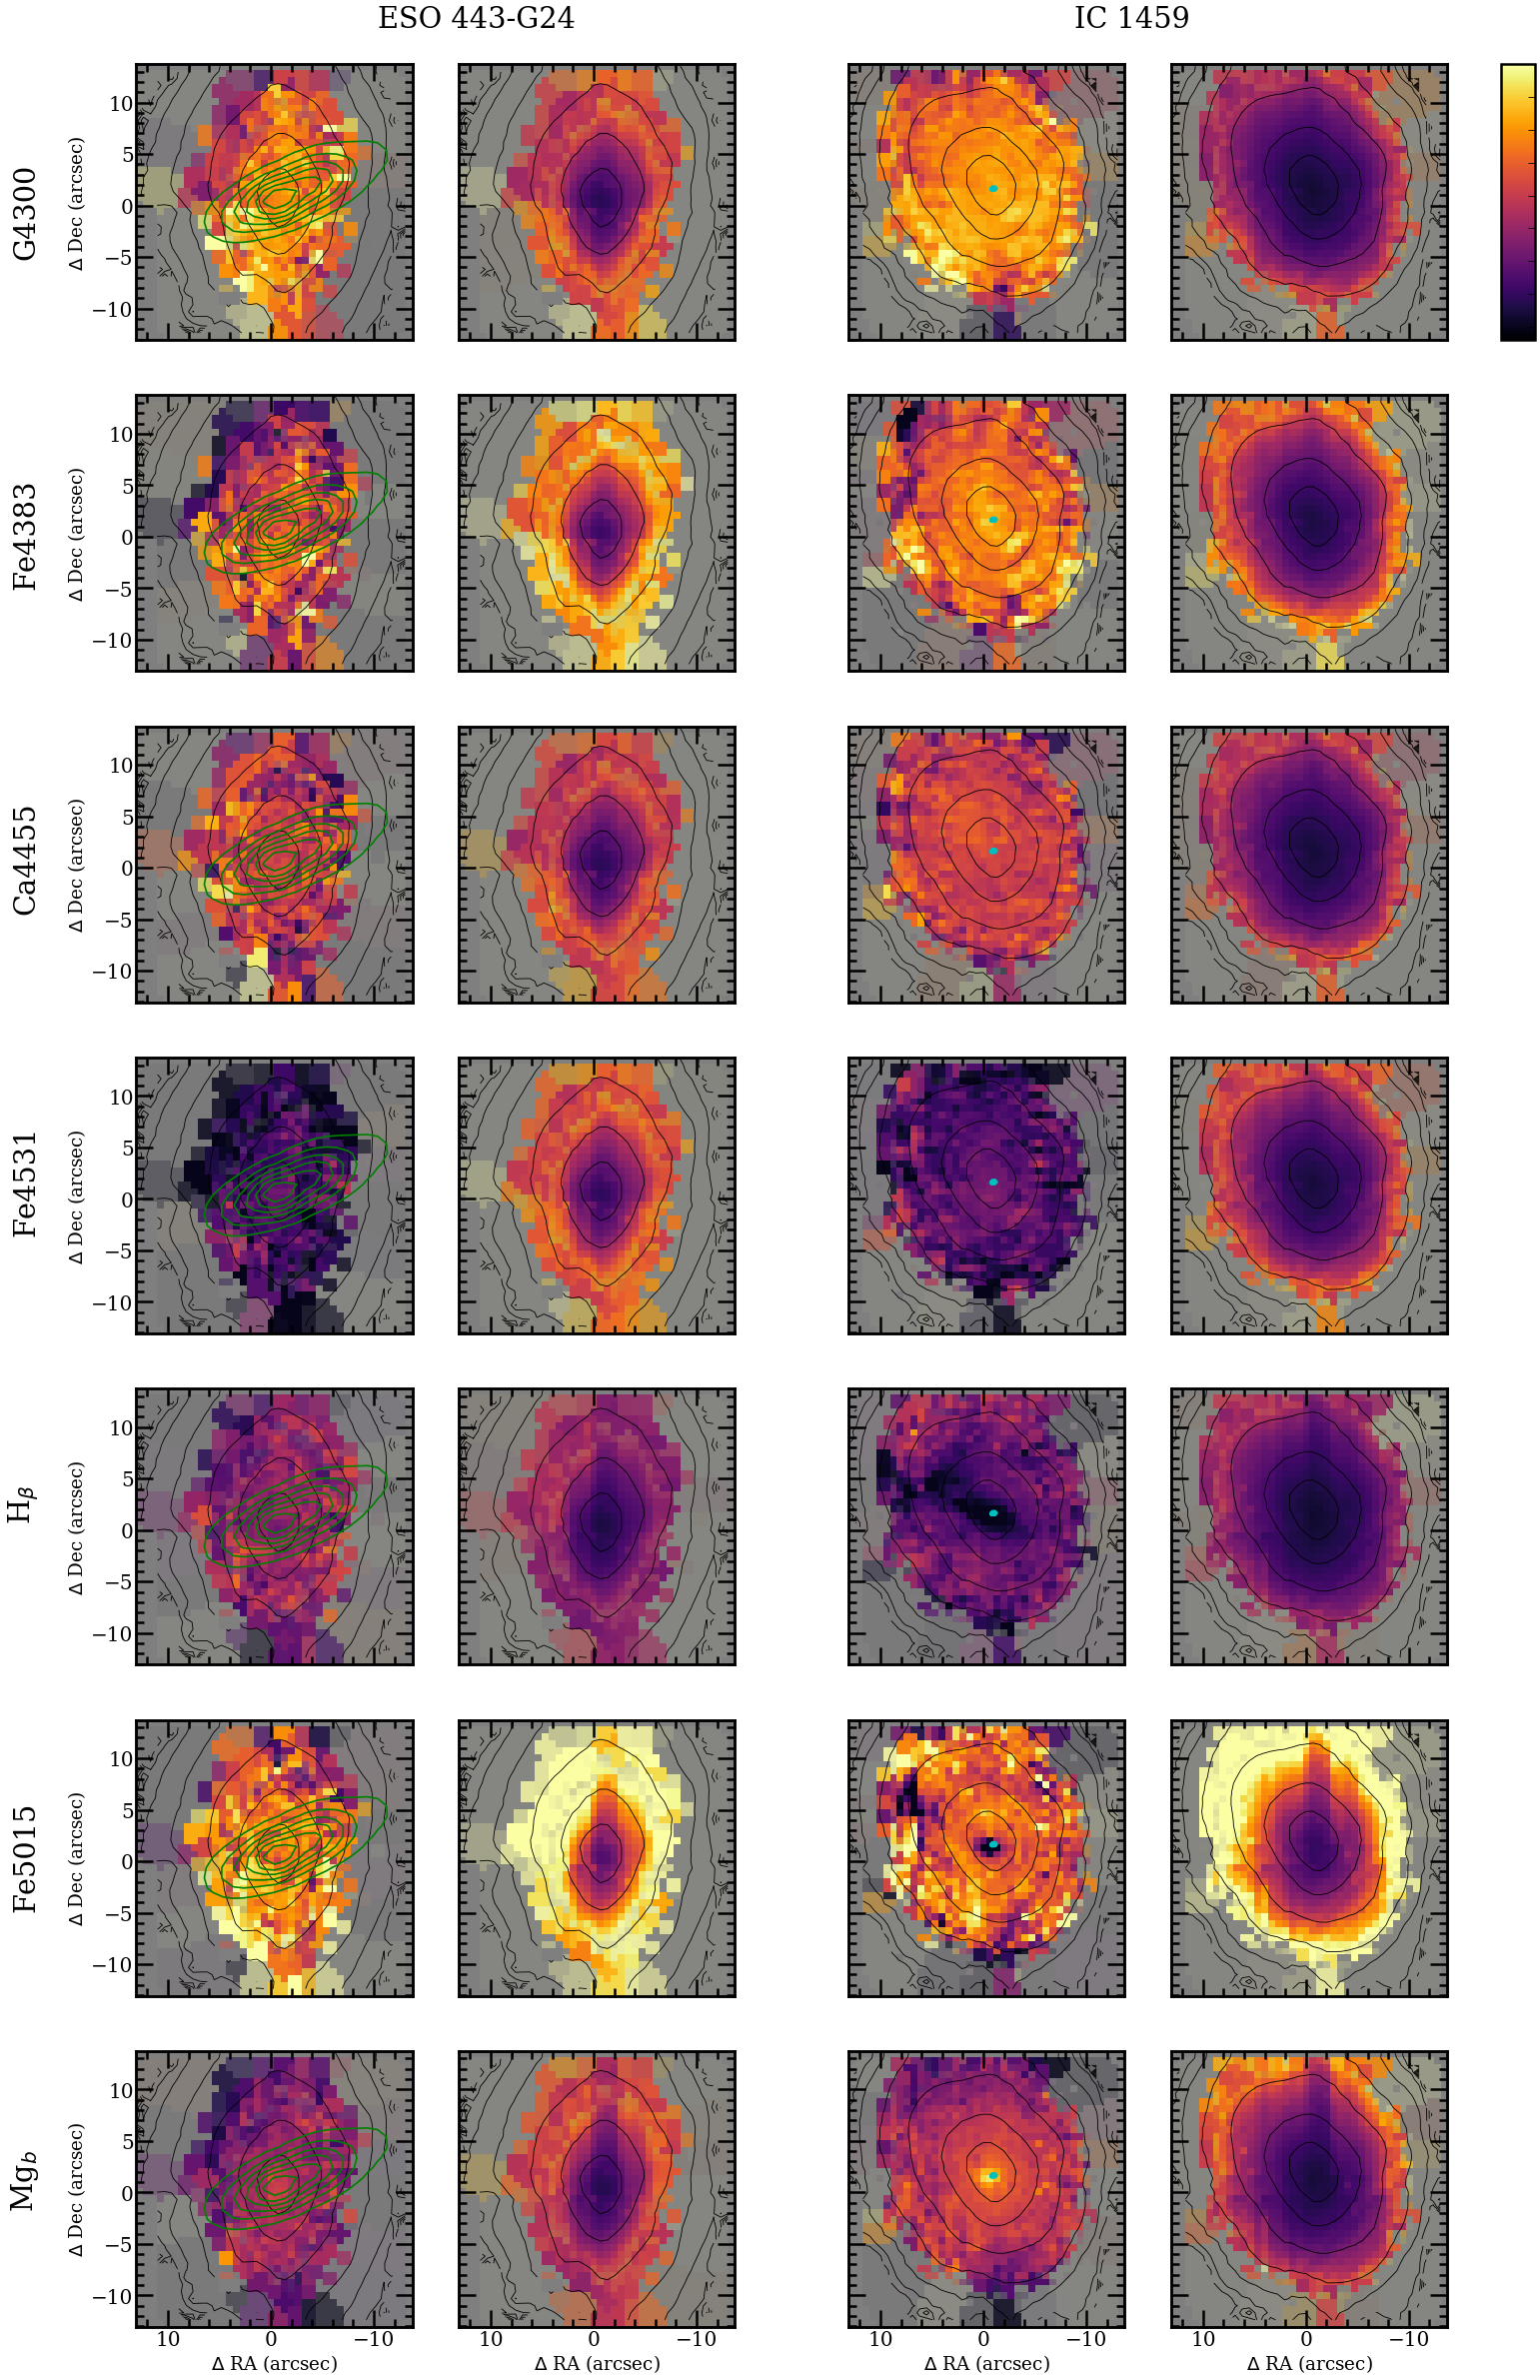
\includegraphics[height=0.94\textheight]{chapter4/vimos/abs1.png}
			\caption[VIMOS absorption line strength maps]{VIMOS stellar kinematic maps: From left to right: ESO 443-G24, ESO 443-G24 uncertainties, IC 1459 and IC 1459 uncertainties. From top to bottom: G4300, Fe4383, Ca4455, Fe4531, H$_\beta$, Fe5015, Mg$_b$. Plots are as in \ref{fig:VIMOS_stellar}. Limits on the color scale are 0-9 \AA  for the line strengths and 0-1 \AA  for the uncertainties.}
			\label{fig:VIMOS_absorption}
		\end{figure}
		\begin{figure}
			\centering
			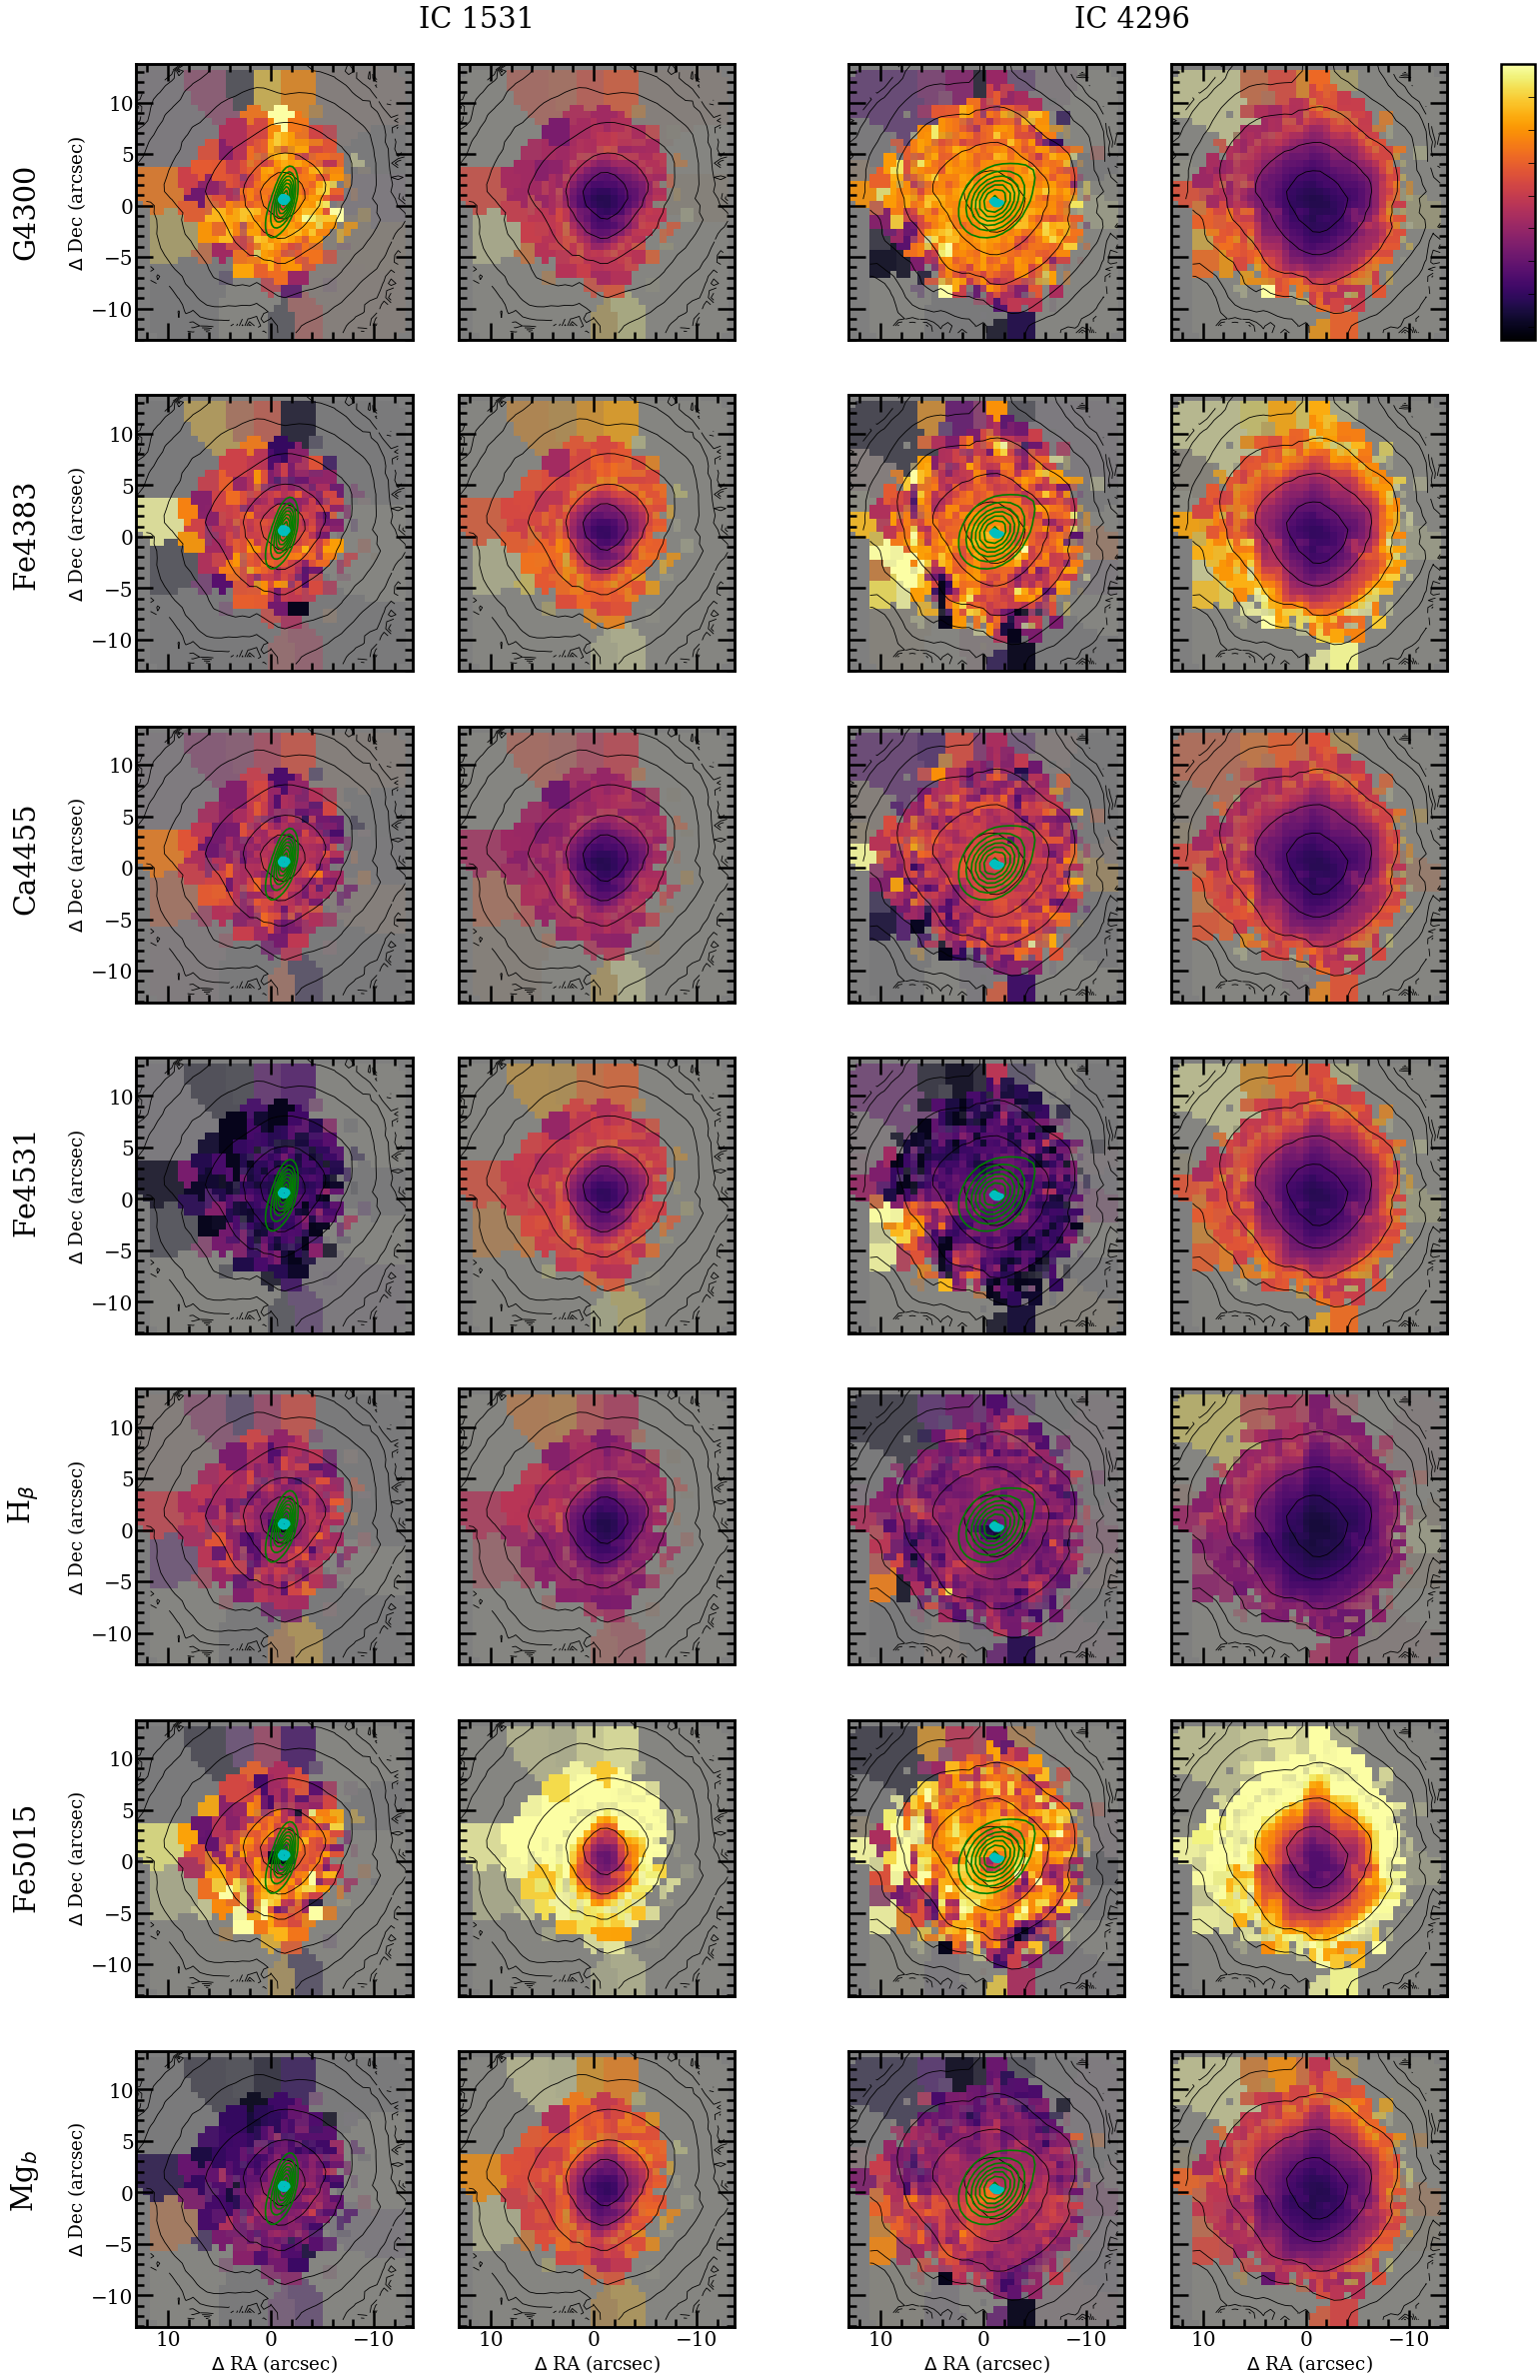
\includegraphics[height=0.94\textheight]{chapter4/vimos/abs2.png}
			\contcaption{continued for IC 1531 and IC 4296.}
		\end{figure}
		\begin{figure}
			\centering
			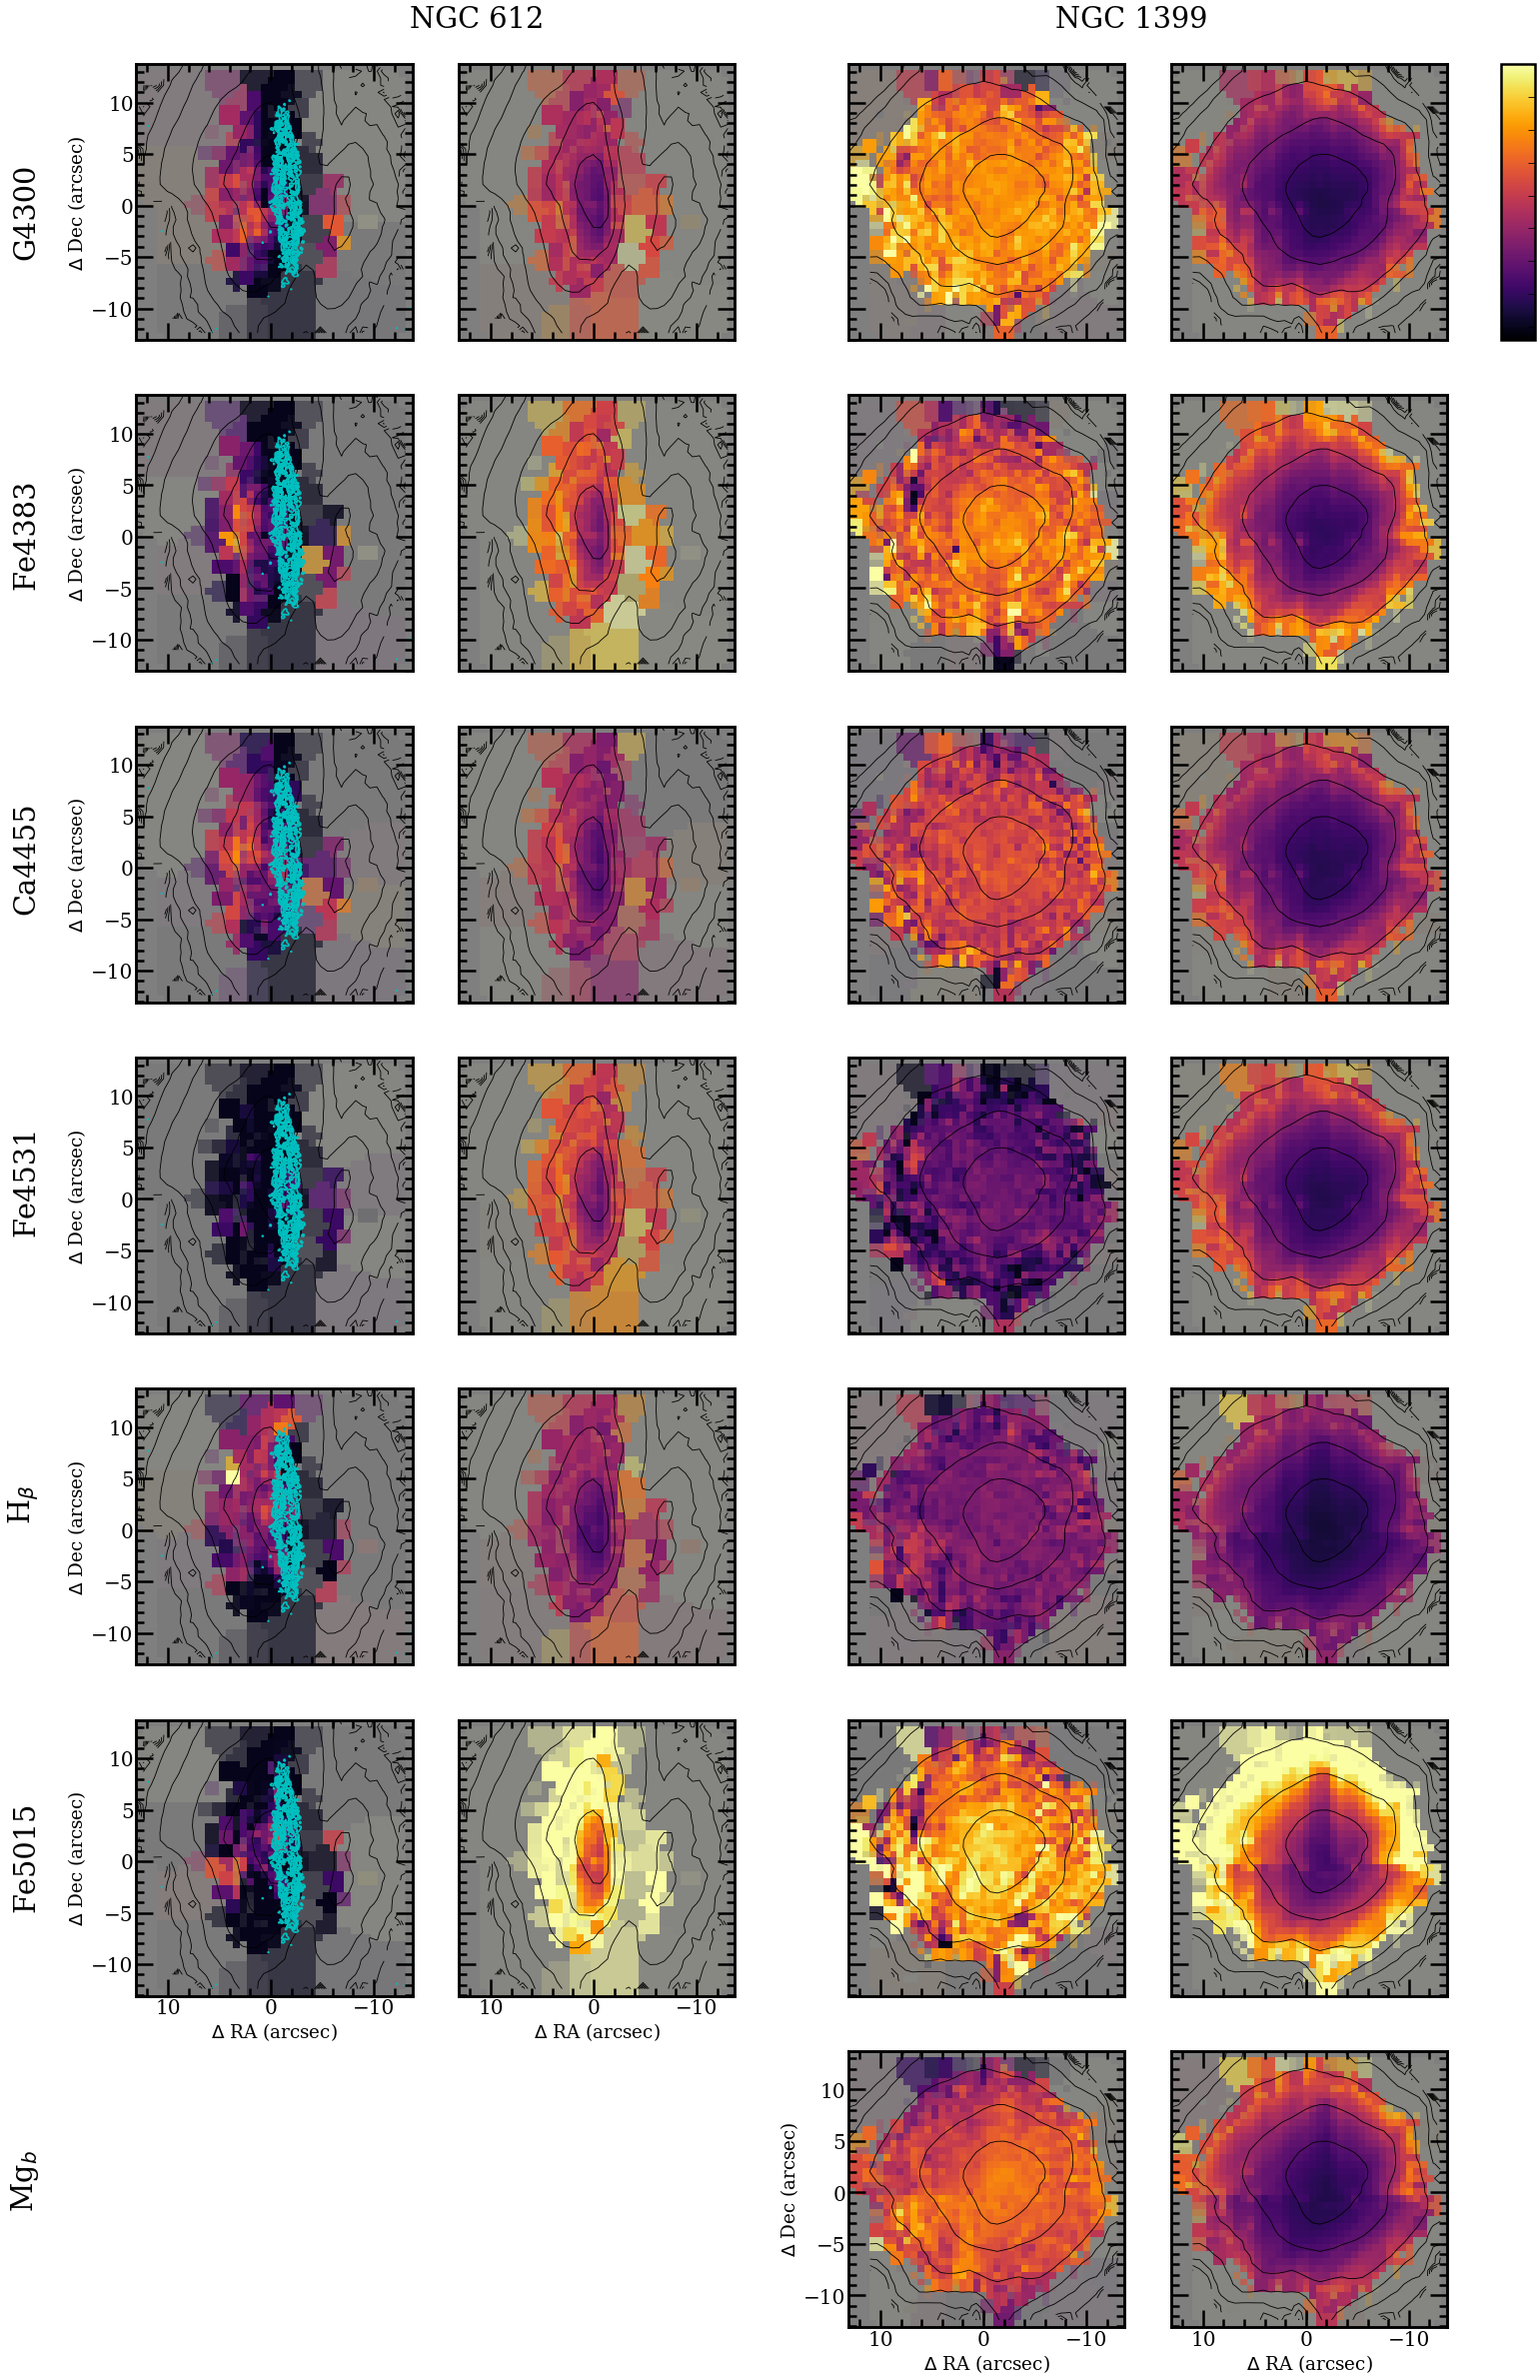
\includegraphics[height=0.94\textheight]{chapter4/vimos/abs3.png}
			\contcaption{continued for NGC 612 and NGC 1399}
		\end{figure}
		\begin{figure}
			\centering
			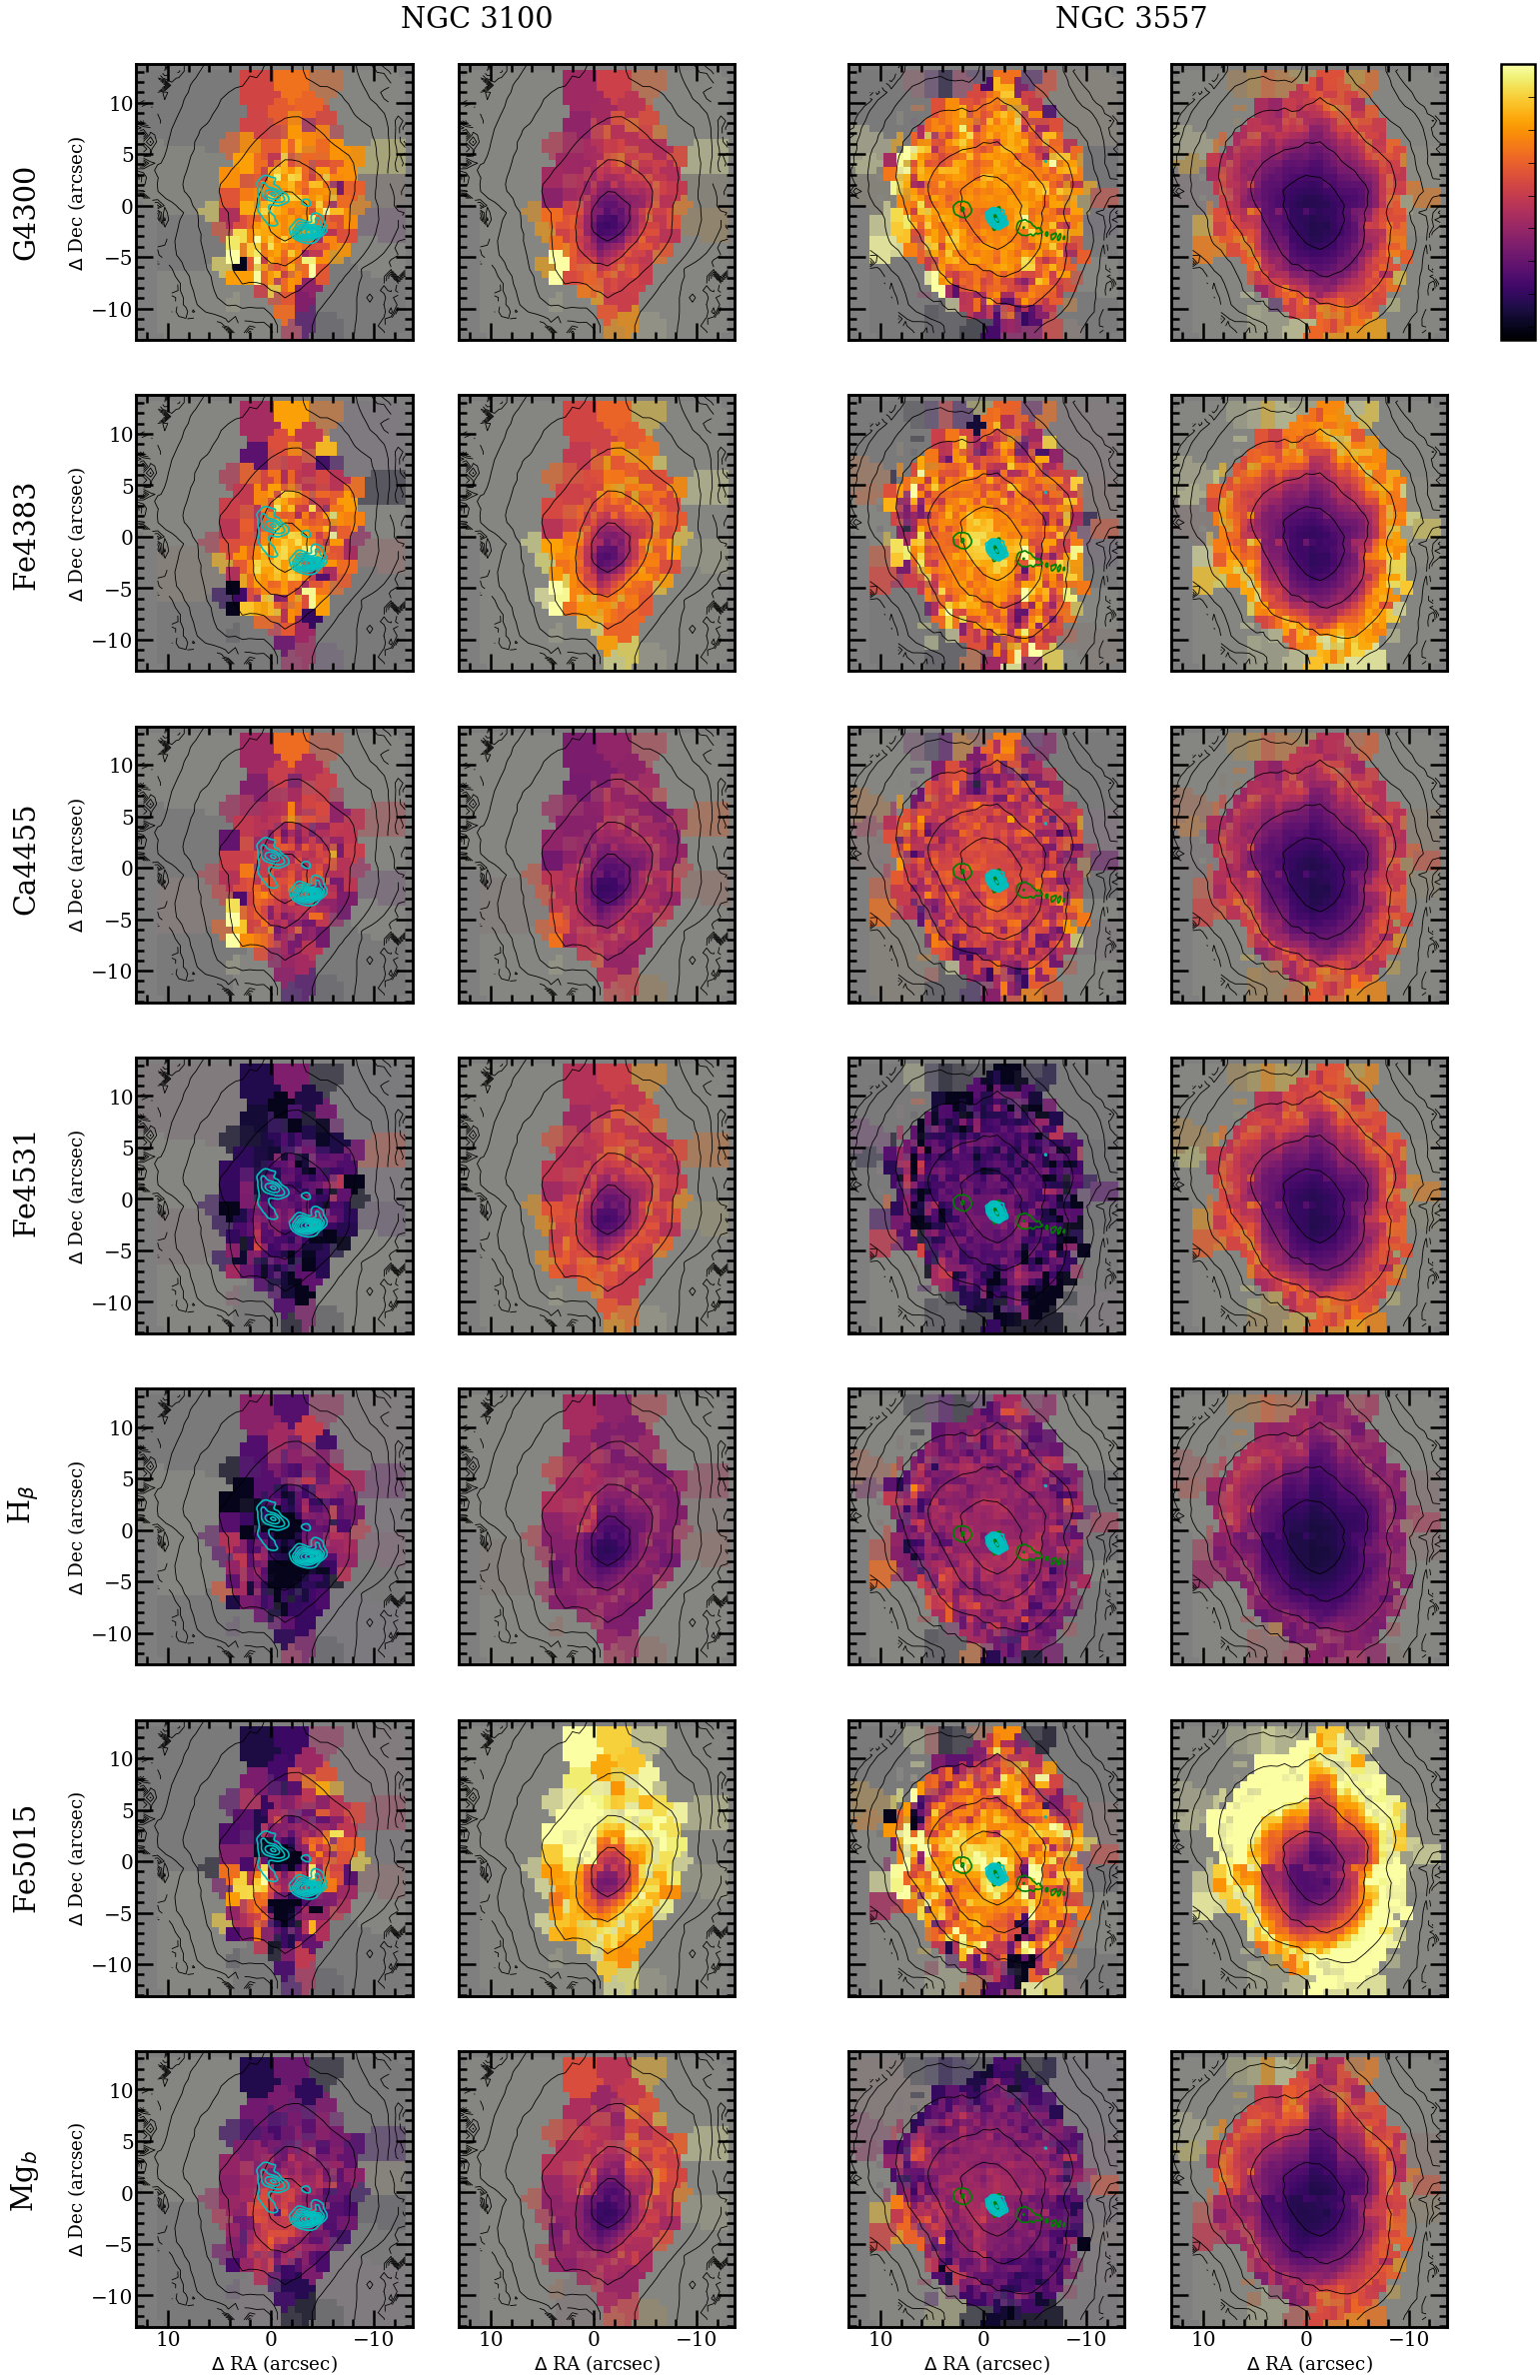
\includegraphics[height=0.94\textheight]{chapter4/vimos/abs4.png}
			\contcaption{continued for NGC 3100 and NGC 3557}
		\end{figure}
		\begin{figure}
			\centering
			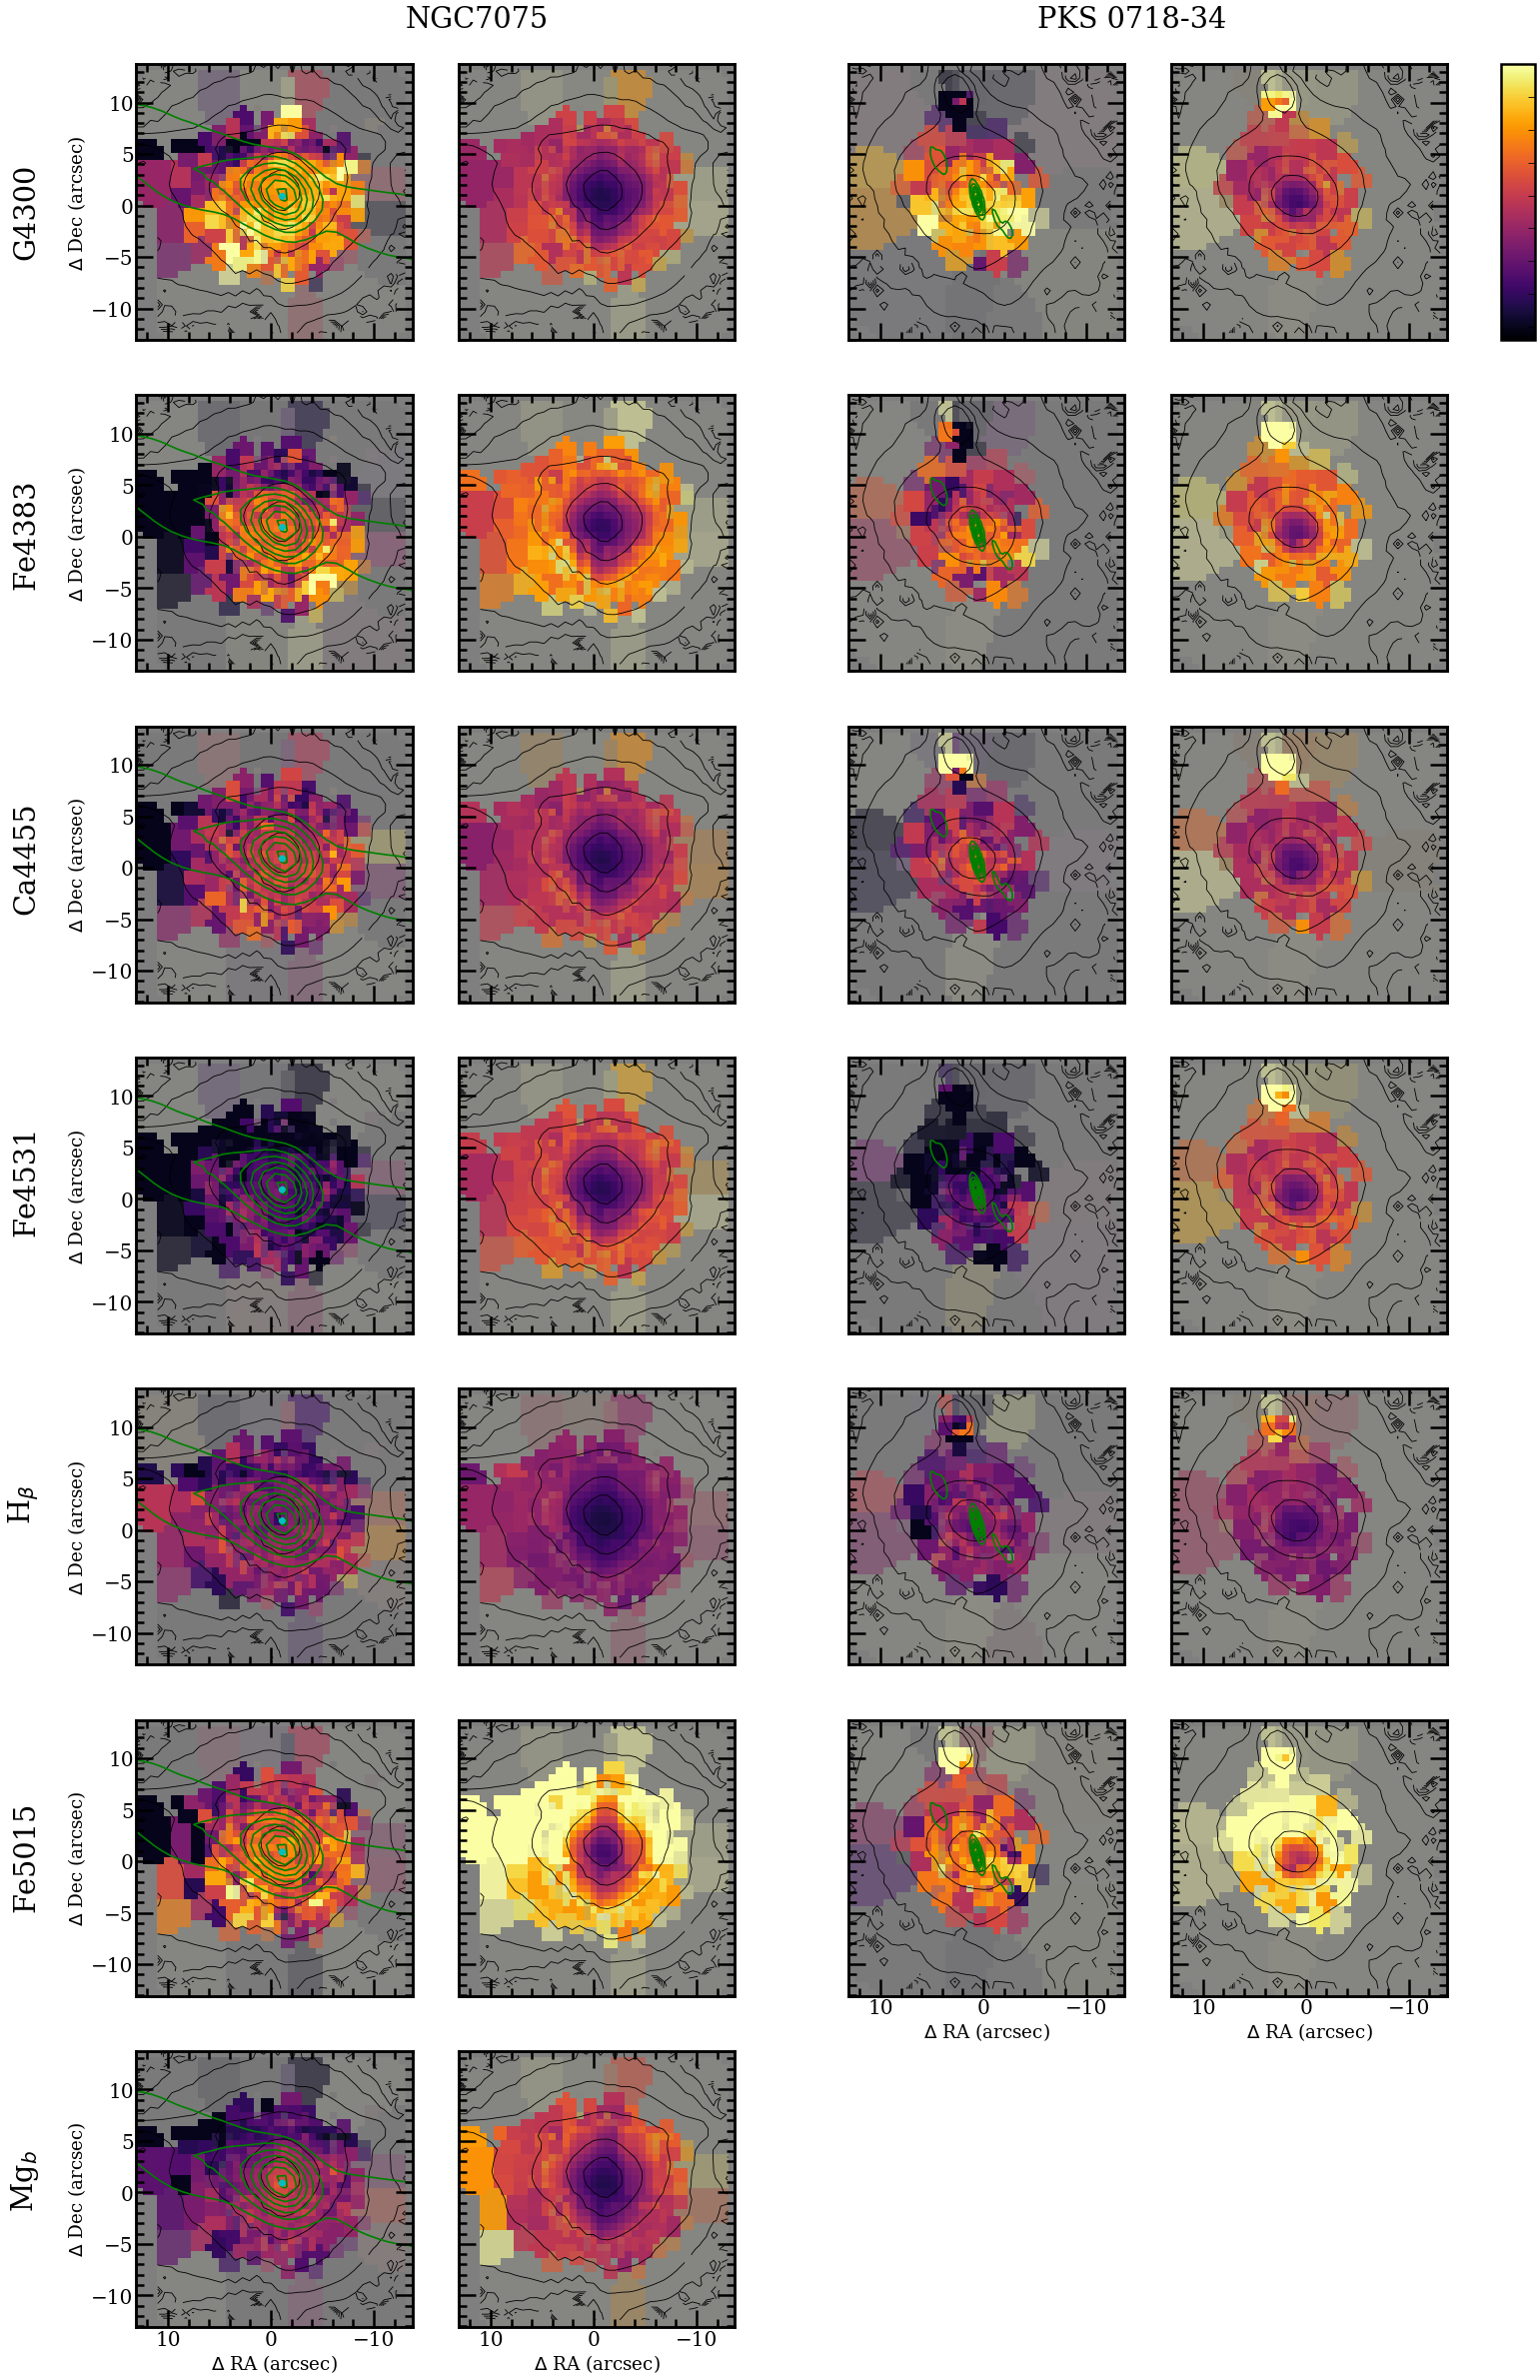
\includegraphics[height=0.94\textheight]{chapter4/vimos/abs5.png}
			\contcaption{continued for NGC 7075 and PKS 718-34}
		\end{figure}

		\begin{figure}
			\centering
			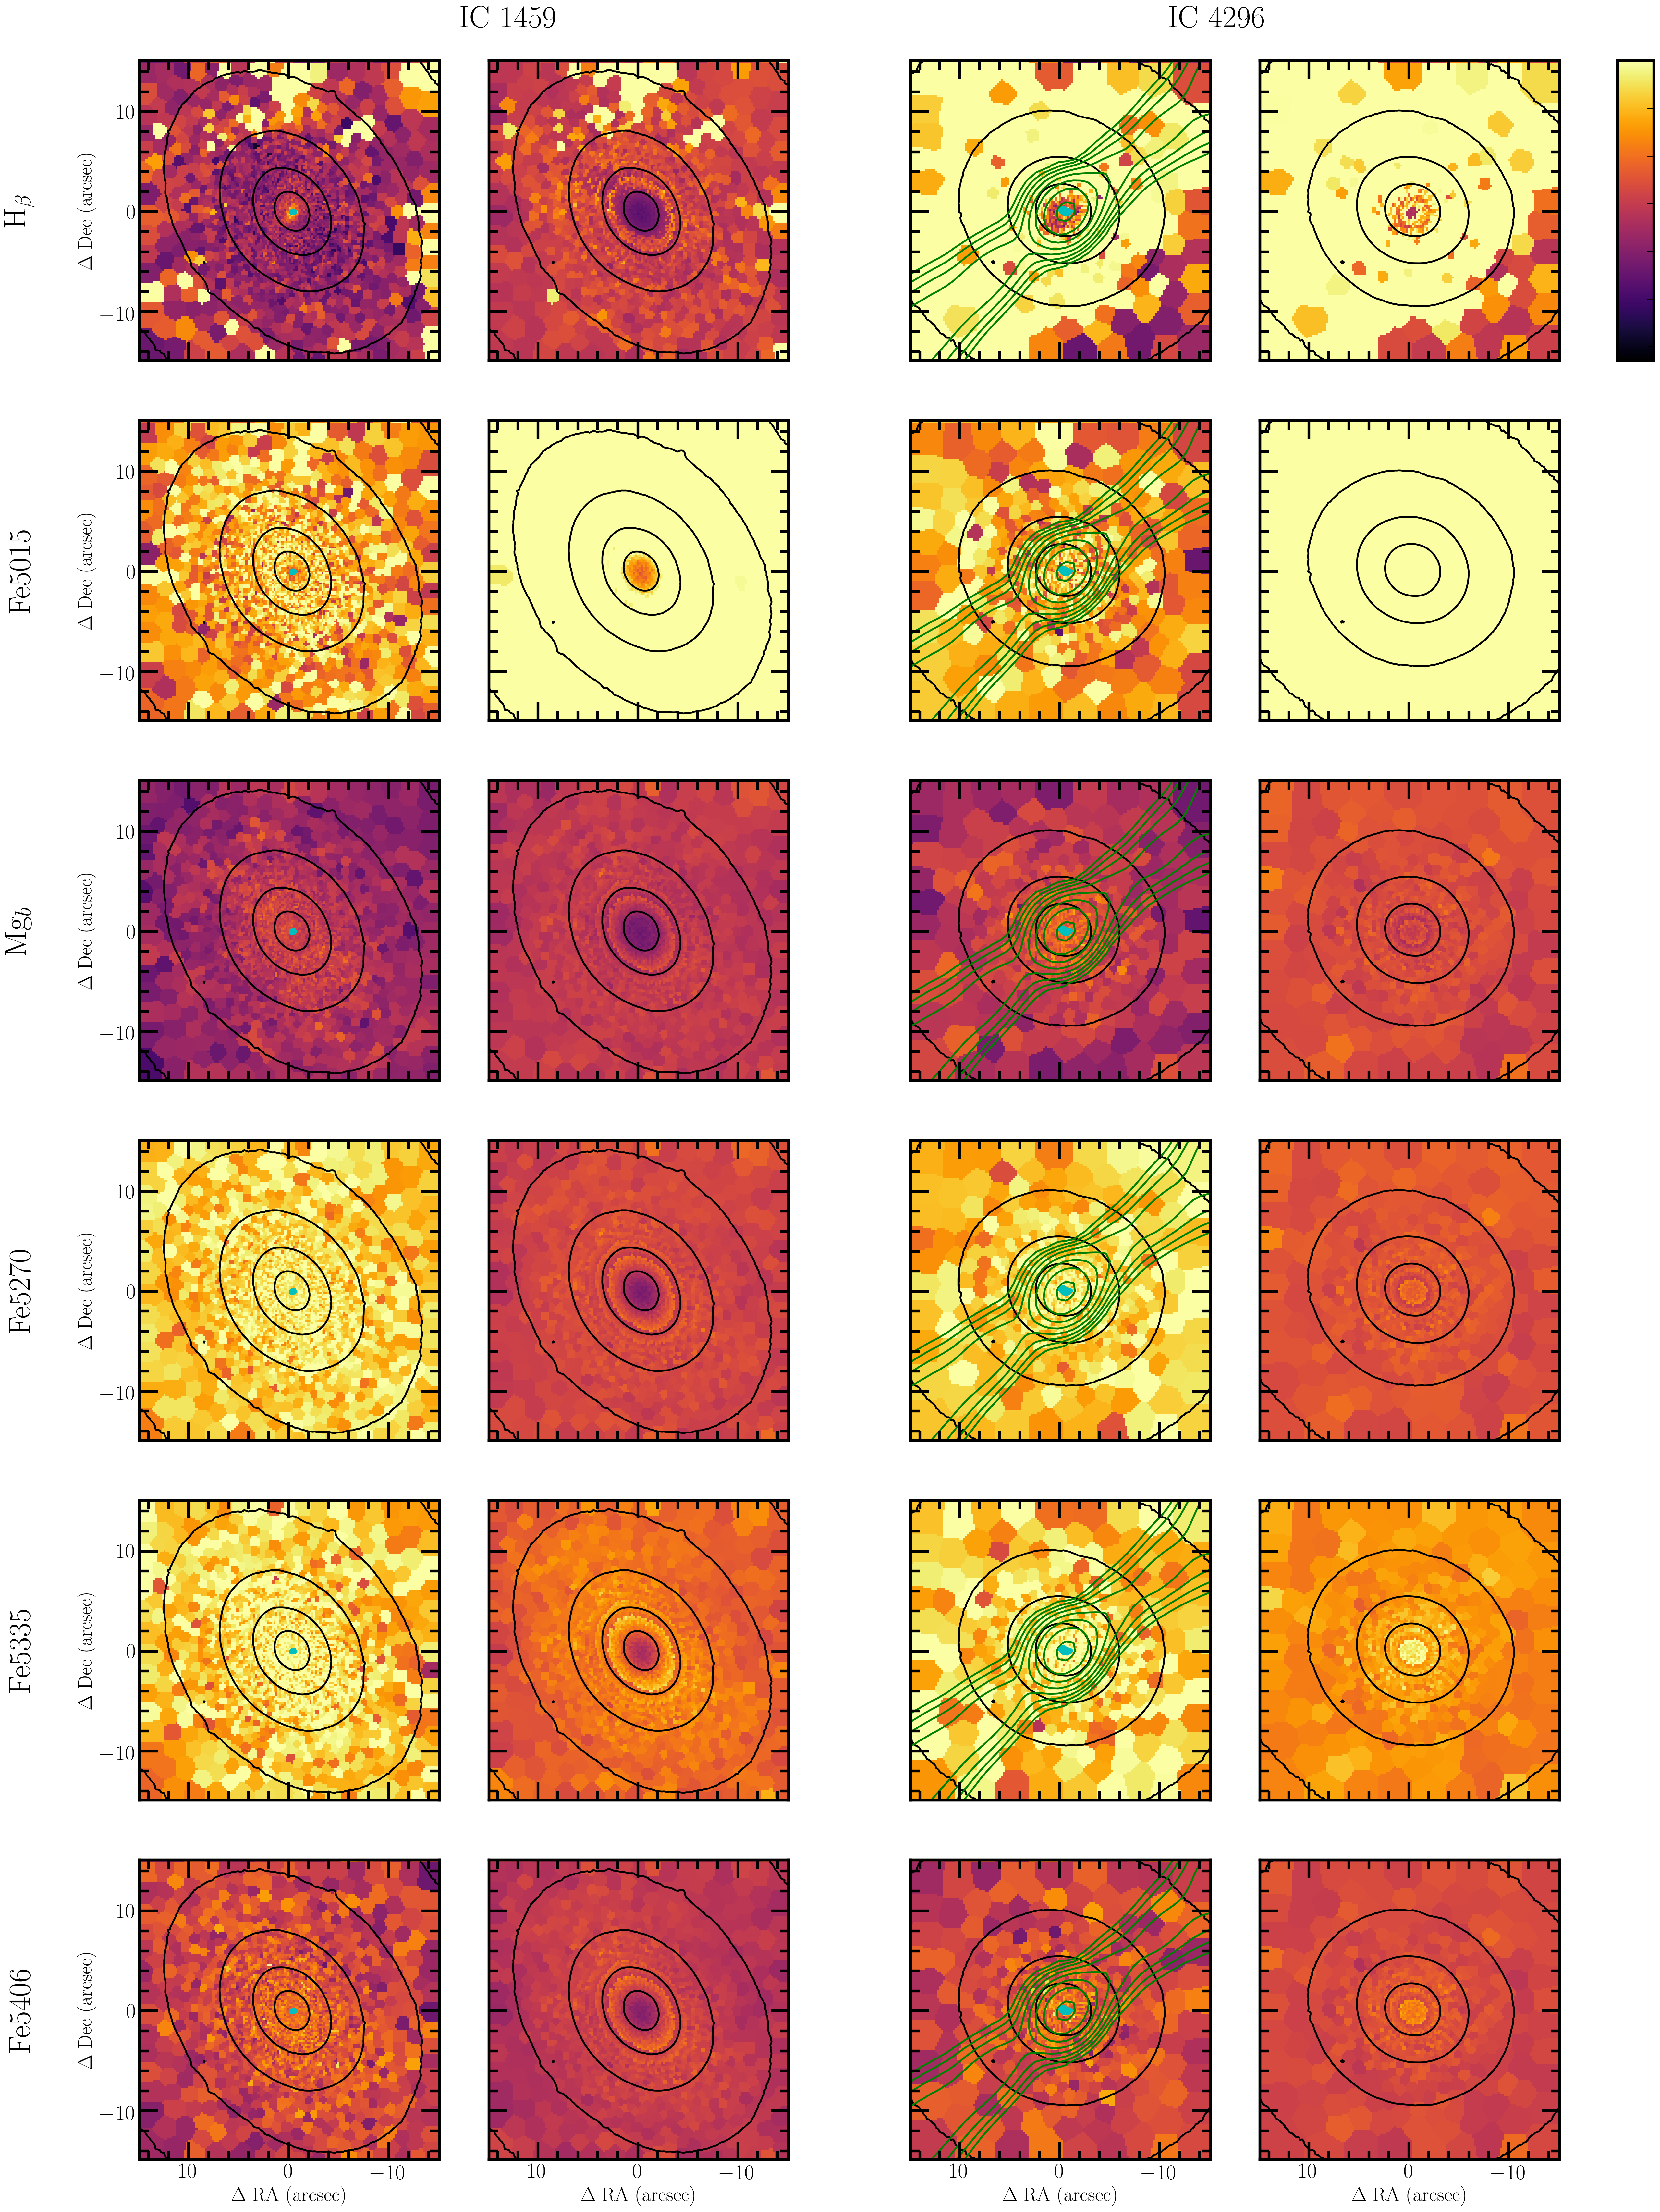
\includegraphics[height=0.94\textheight]{chapter4/muse/abs1.png}
			\caption[MUSE absorption line strength maps]{MUSE stellar kinematic maps: From left to right: IC1459, IC1459 uncertainties, IC4296 and IC4296 uncertainties. Plots are as in Figure \ref{fig:VIMOS_stellar}. Limits on the color scale are 0-9 \AA  for the line strengths and 0-1 \AA  for the uncertainties.}
			\label{fig:MUSE_absorption}
		\end{figure}
		\begin{figure}
			\centering
			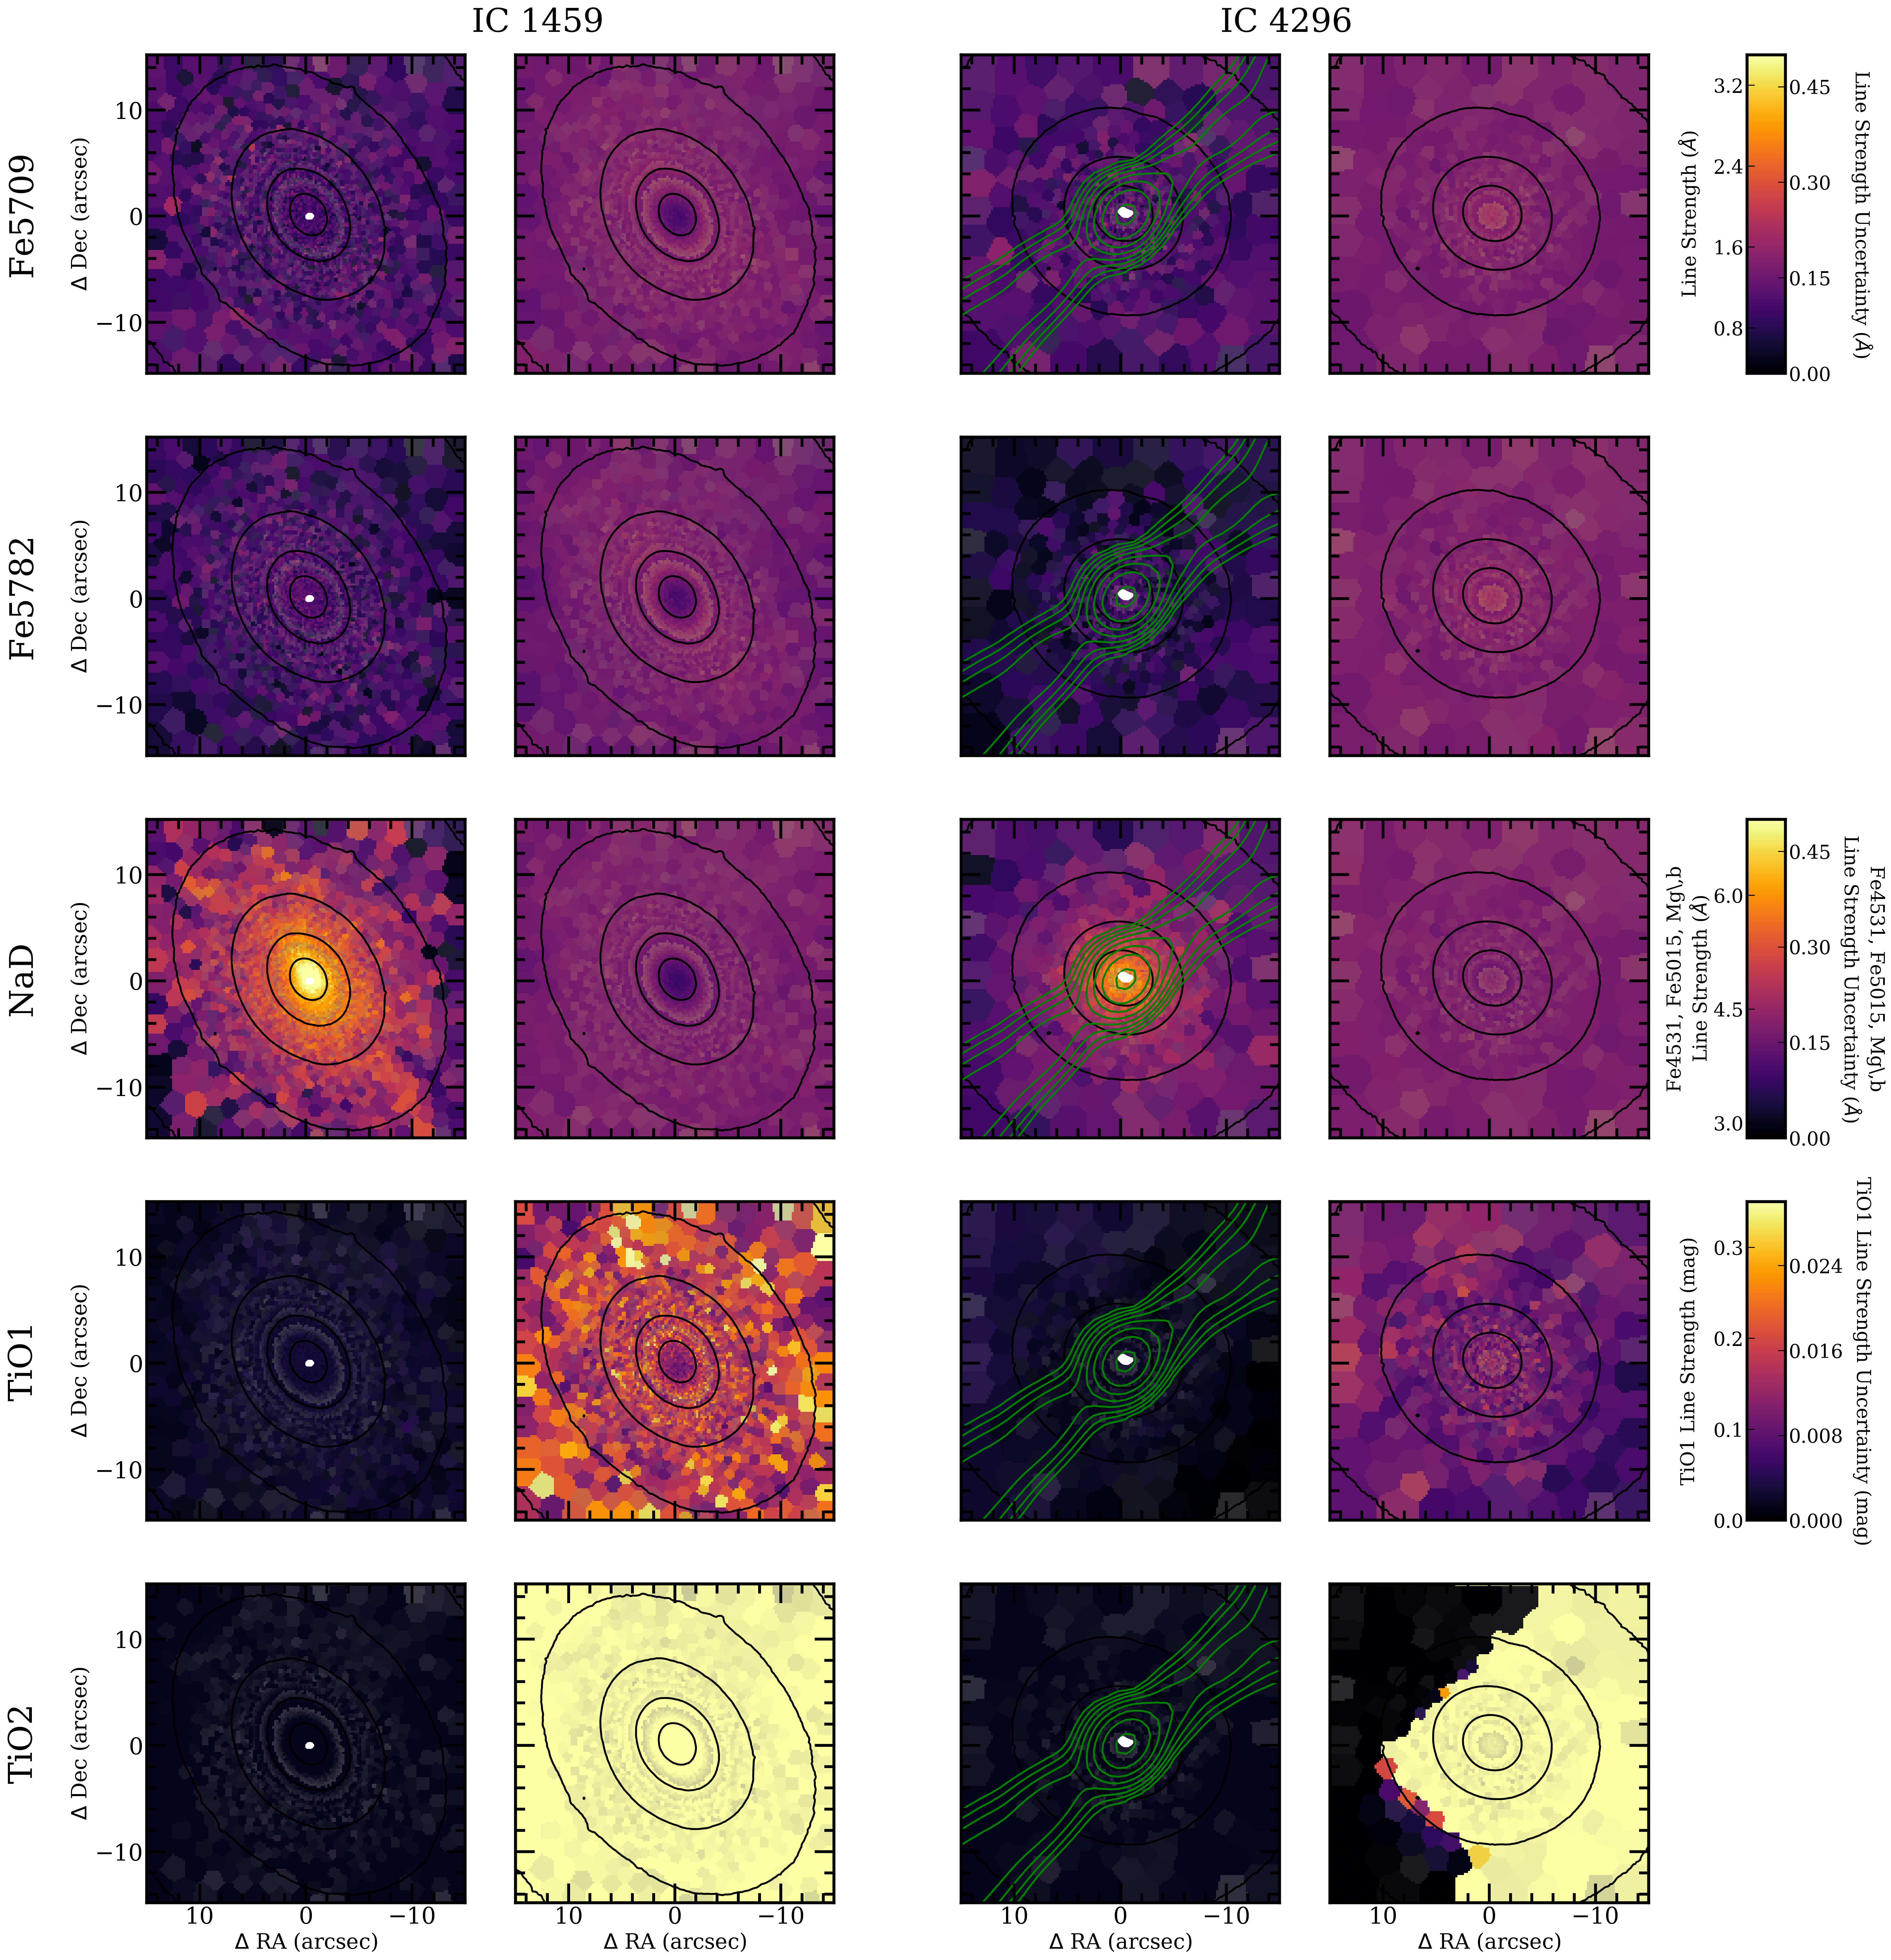
\includegraphics[height=0.54\textheight]{chapter4/muse/abs1b.png}
			\contcaption{continued: From top to bottom: Fe5782, NaD, TiO1, TiO2. Plots are as in \ref{fig:VIMOS_stellar}. Limits on the color scale are 0-9 \AA  for the line strengths and 0-1 \AA  for the uncertainties and \_\_\_-\_\_\_ mag for TiO1 and TiO2 line strengths and \_\_\_-\_\_\_ mag for the uncertainty in TiO1 and TiO2.}
		\end{figure}
		\begin{figure}
			\centering
			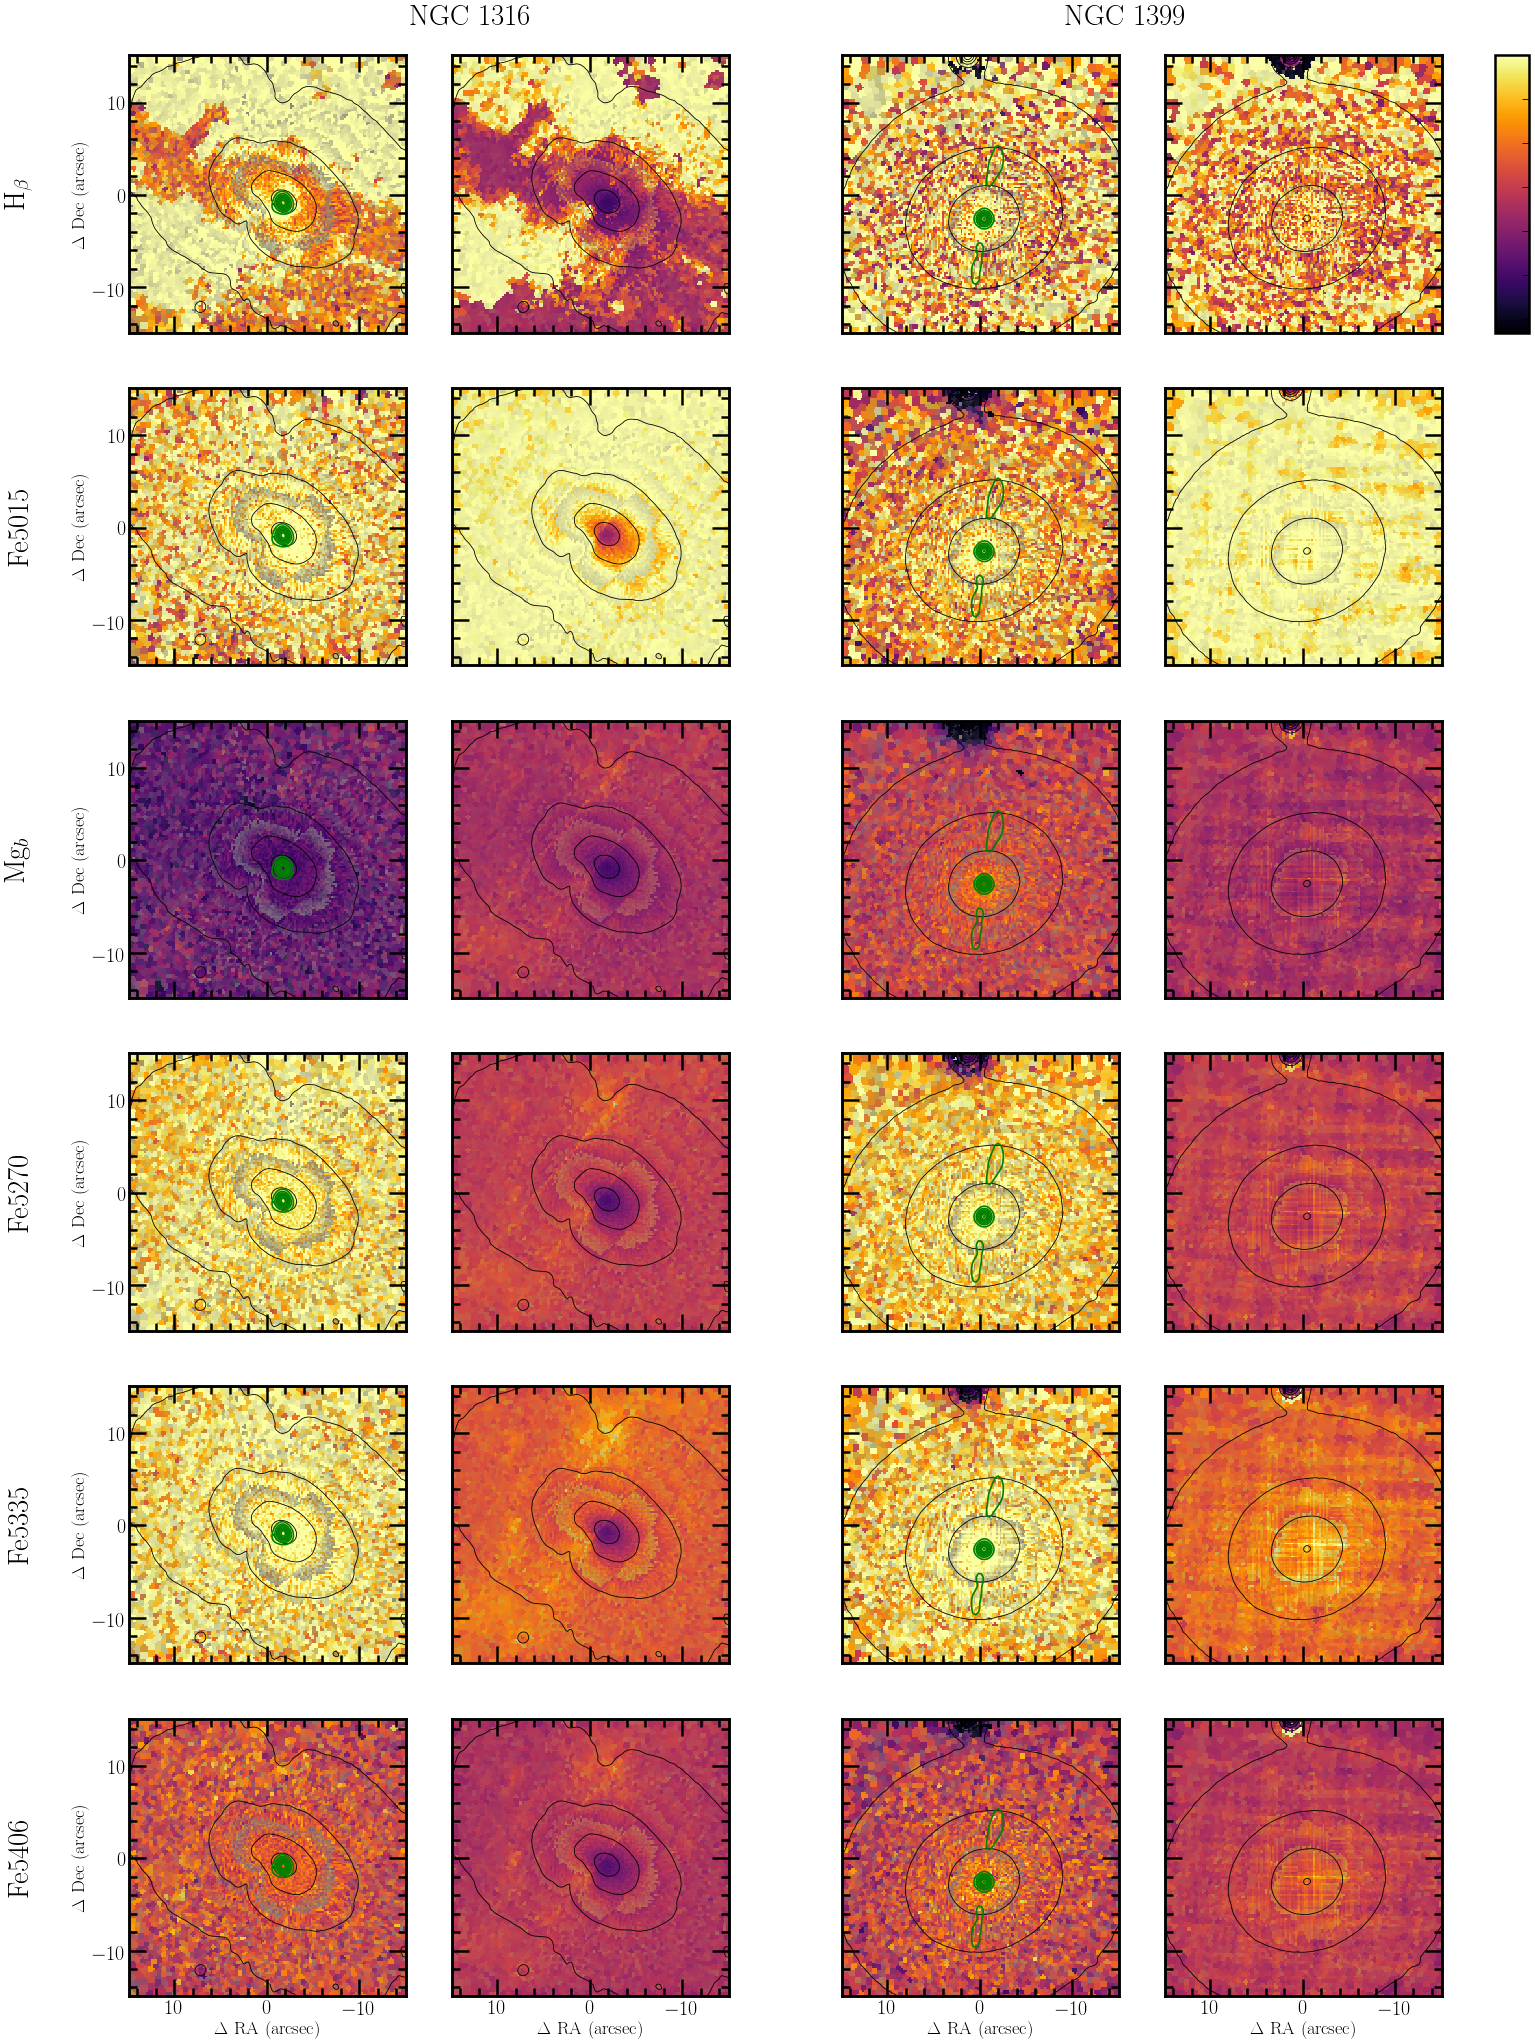
\includegraphics[height=0.94\textheight]{chapter4/muse/abs2.png}
			\contcaption{continued for NGC1316 and NGC1399.}
		\end{figure}
		\begin{figure}
			\centering
			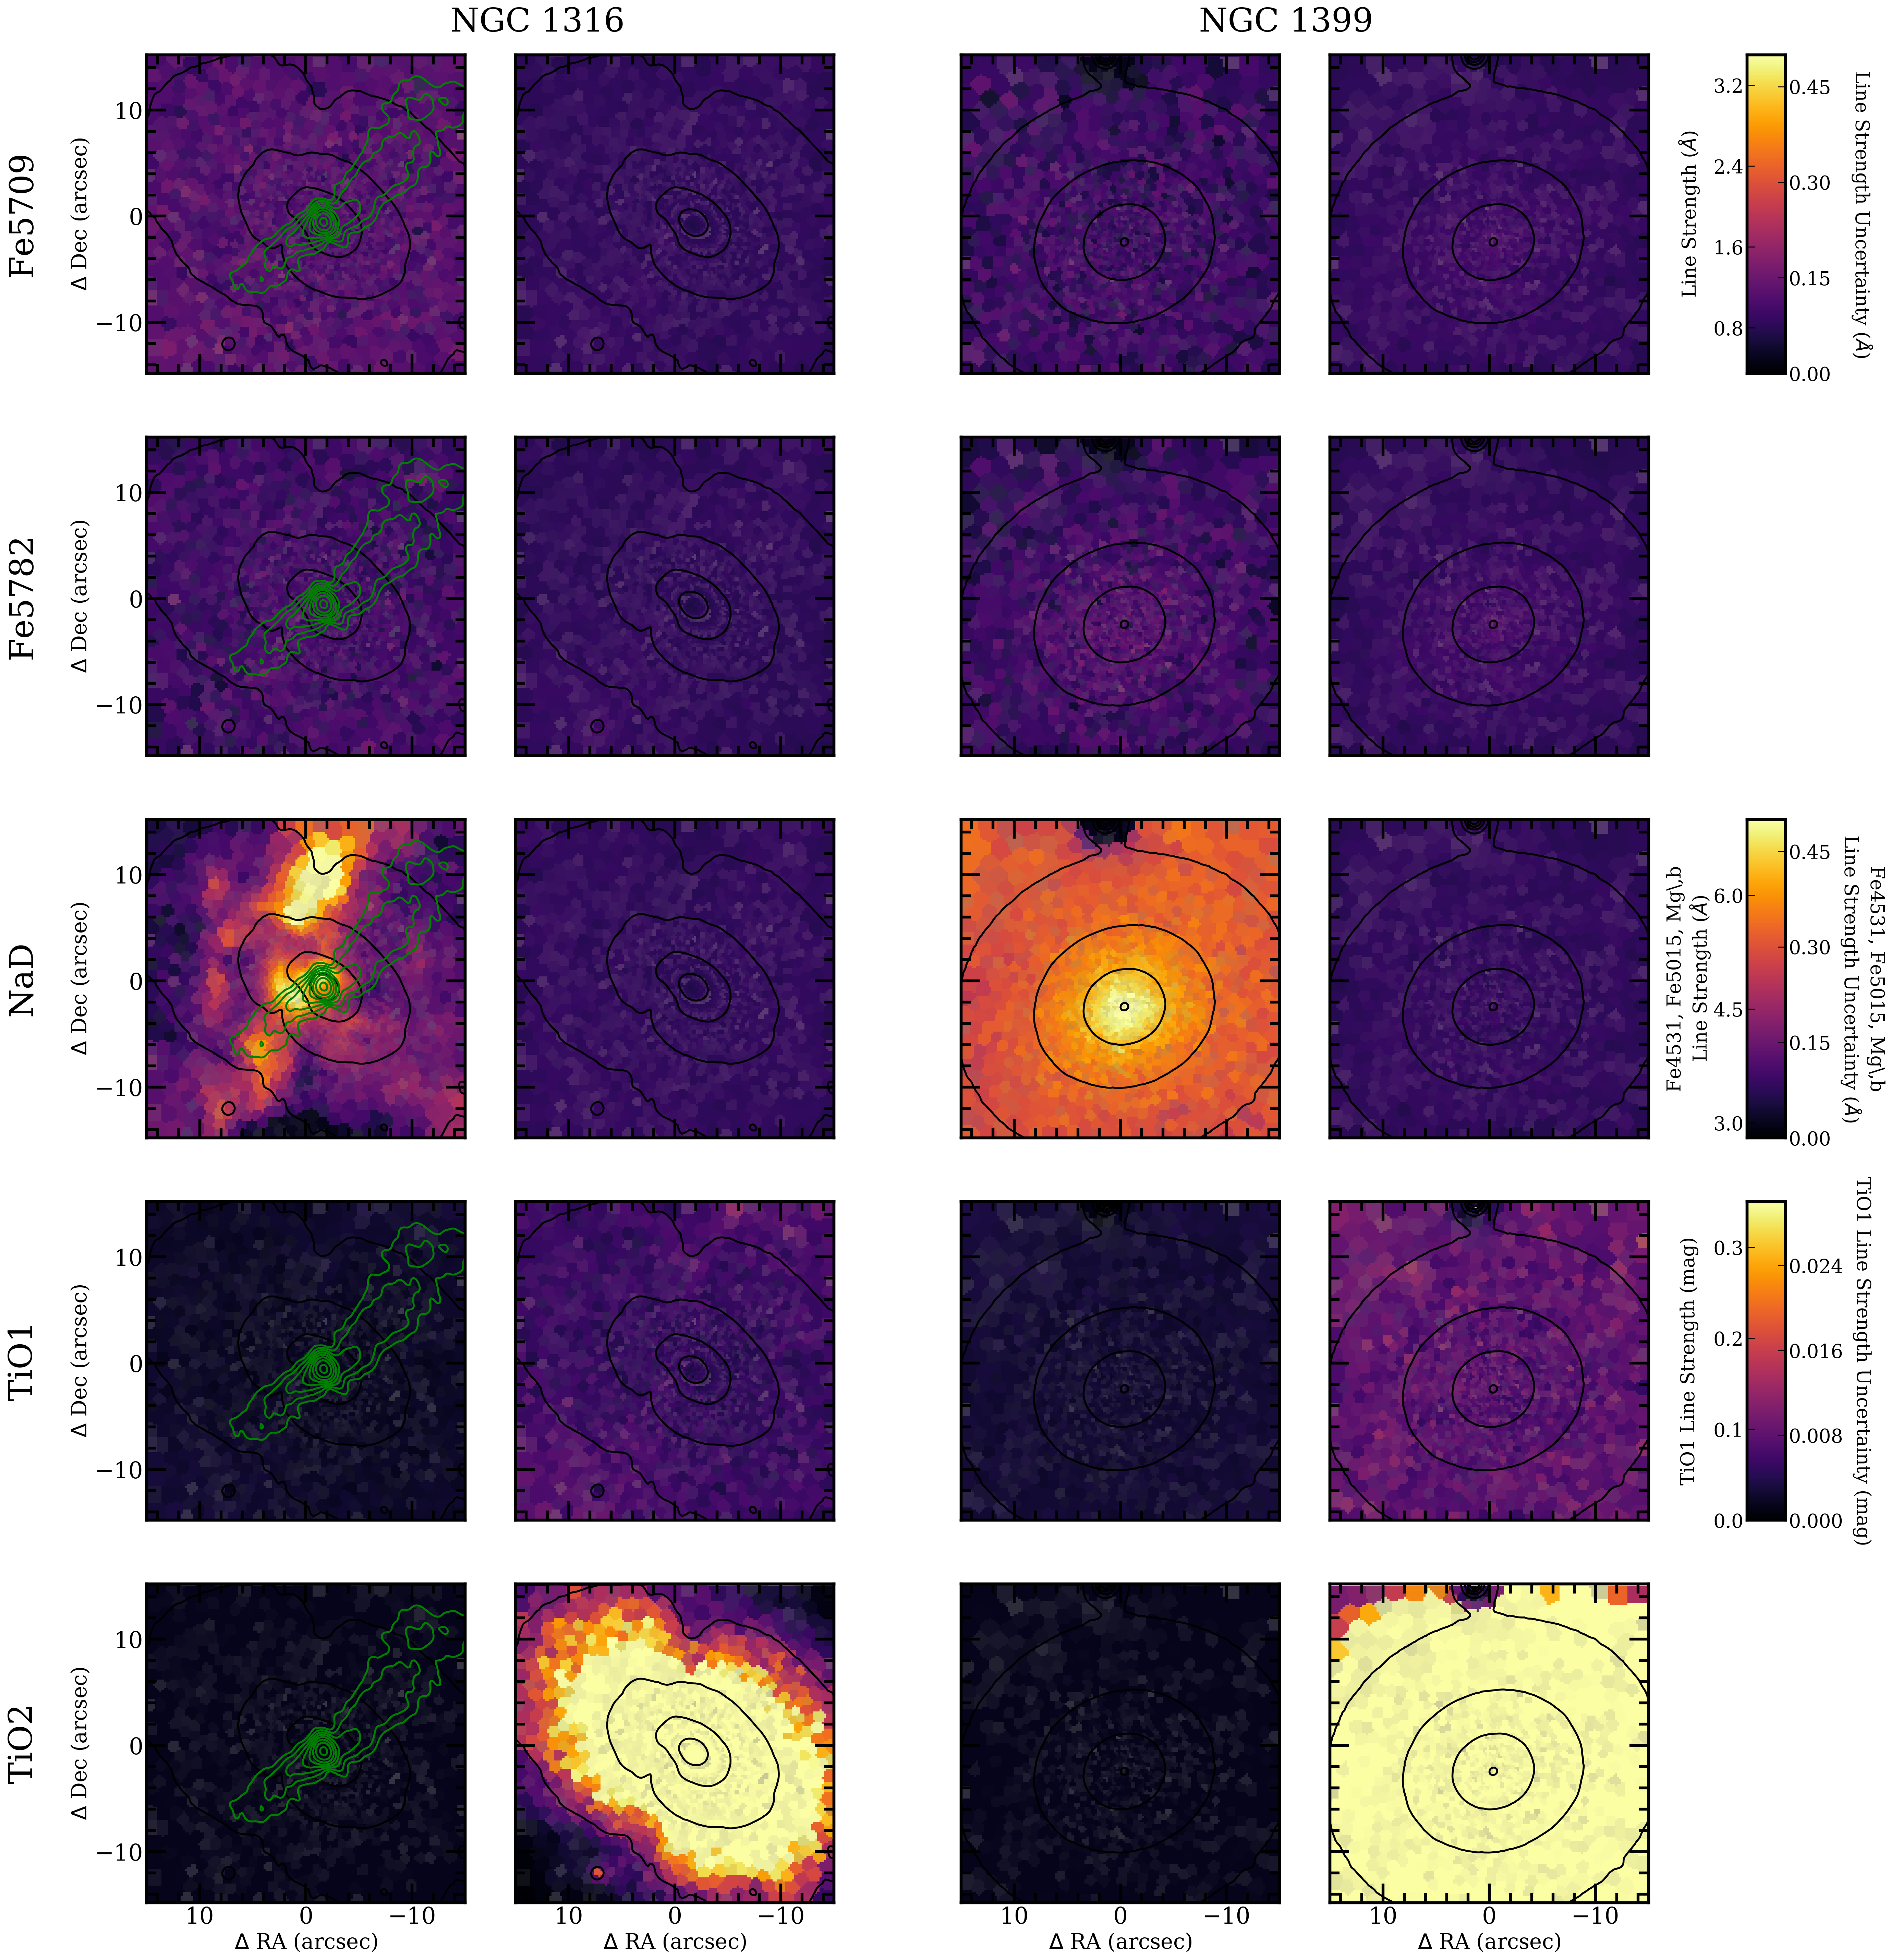
\includegraphics[height=0.54\textheight]{chapter4/muse/abs2b.png}
			\contcaption{continued for NGC1316 and NGC1399.}
		\end{figure}


	Comparison to the literature is made difficult by the inhomogeneous nature of corrections applied by different authors.Accounting for emission lines from the interstellar medium (ISM) or velocity dispersion are two examples. We use the line index system (LIS) by \citet{Vazdekis2010} instead of the popular Lick/IDS system \citep{Faber1985, Worthey1994}. This is because the Lick/IDS system is based on non-flux calibrated spectra from the IDS and Cassegrain spectrograph on the Shane telescope (Lick Observatory) which has a relatively low and wavelength dependent resolution. When using other instruments with the Lick/IDS system it is necessary to calibrate the observations by performing empirical corrections to correct for the uncalibrated continuum of Lick/IDS. This requires the observation of standard stars with the same instrumental set up as the main observations in order to make comparisons to the measurements from the IDS spectrograph. Since this was not requested as part of the observing strategy with VIMOS we are not able to do this: a later proposal would not have worked since VIMOS was substantially upgraded in the intervening time period. Due to the low resolution and poor data quality on which the Lick/IDS system is based, we believe that it has had its time and that the community should be making a concerted effort to use alternative systems. As there is a lack of non-Lick/IDS system measurements: we used the empirical functions provided by \citet{Vazdekis2010} to translate between Lick/IDS and LIS systems\footnote{The transformation from Lick/IDS to the LIS system is available at http://www.iac.es/proyecto/miles/pages/line-index-system-lis/transformations.php.} to allow comparison to the literature. 


	Finally, we note that only the H$_\beta$ emission line is corrected for in some of the literature, despite [OIII] often being the strongest emission line for ETGs. This effects the reliability of the Fe5015 and Mb$_b$ absorption indices as the [OIII] and [NI] doublets fall within them respectively. They vary as to whether they fall within the index band or the continuum bands and the effect depends on the relative difference in the kinematics of the stars (which result in the absorption features) and the ISM (which results in the emission lines). Other papers correct for only H$_\beta$ and [OIII]. In order to make accurate comparisons to the literature, we mimic the corrections used in the paper chosen for comparison: i.e. we only correct for the emission lines the paper corrects for and apply the same aperture corrections as in the paper. All emission lines (given in table \ref{tab:EmissionLines}) are removed for our quoted measurements and maps. Table \ref{tab:litAbsorption} sums up our comparison to the literature. Here we note that in the case of comparison to \citet{Rampazzo2005}, G4300 has a very large offset. We suggest that this index is extremely sensitive to the velocity dispersion due to the steep nature of the pseudo-continuum: a difference of $30 \, \mathrm{km \, s^{-1}}$ can effect the corrected index value by $\sim 2 \, \mathrm{\AA}$. For the comparison to \citet{Vazdekis2010}, we analyzed the SAURON data set\footnote{SARUON data is available at: http://www.strw.leidenuniv.nl/sauron/.} \citep{Emsellem2004} using the same pipeline we have developed for our sample. 

	\begin{table}
		\centering
	\begin{threeparttable}
		\caption{Comparisons of measured absorption line indices to the literature.}
		\label{tab:litAbsorption}
		\begin{tabular*}{0.8\textwidth}{@{\extracolsep{\fill}}l r r r}
			\hline
			\hline
			Index 		& \multicolumn{1}{c}{N$_\mathrm{gals}$} & \multicolumn{1}{c}{Offset} & \multicolumn{1}{c}{Dispersion} \\
						& 		&\multicolumn{1}{c}{\AA}& \multicolumn{1}{c}{\AA} \\
			\hline
			\multicolumn{4}{c}{\citet{Vazdekis2010} (SAURON)} \\
			\hline
			H$_\beta$ 	& 46		& -0.02\leavevmode\phantom{0}& 0.25\leavevmode\phantom{0}	\\
			Fe5015		& 46		& 0.66\leavevmode\phantom{0}& 0.34\leavevmode\phantom{0}	\\
			Mg$_b$ 		& 46		& 0.06\leavevmode\phantom{0}& 0.33\leavevmode\phantom{0}	\\
			\hline
			\multicolumn{4}{c}{\citet{Rampazzo2005} (VIMOS)} \\
			\hline
			G4300 		& 3 		& 2.29\leavevmode\phantom{0}& 0.11\leavevmode\phantom{0}	\\
			Fe4383 		& 3 		& 0.39\leavevmode\phantom{0}& 0.23\leavevmode\phantom{0}	\\
			Ca4455 		& 3 		& -0.19\leavevmode\phantom{0}& 0.09\leavevmode\phantom{0}	\\
			Fe4531 		& 3 		& 0.16\leavevmode\phantom{0}& 0.26\leavevmode\phantom{0}	\\
			H$_\beta$ 	& 3 		& 0.17\leavevmode\phantom{0}& 0.12\leavevmode\phantom{0}	\\
			Fe5015 		& 3 		& -0.73\leavevmode\phantom{0}& 0.48\leavevmode\phantom{0}	\\
			Mg$_b$ 		& 3 		& -0.43\leavevmode\phantom{0}& 0.17\leavevmode\phantom{0}	\\
			\hline
			\multicolumn{4}{c}{\citet{Rampazzo2005} (MUSE)} \\
			\hline
			H$_\beta$ 	& 2 		& -0.28\leavevmode\phantom{0}& 0.17\leavevmode\phantom{0}	\\ 
			Fe5015 		& 2 		& 0.87\leavevmode\phantom{0}& 0.34\leavevmode\phantom{0}	\\ 
			Mg$_b$ 		& 2 		& 0.31\leavevmode\phantom{0}& 0.14\leavevmode\phantom{0}	\\
			Fe5270 		& 2 		& -0.11\leavevmode\phantom{0}& 0.15\leavevmode\phantom{0}	\\
			Fe5335 		& 2 		& 0.08\leavevmode\phantom{0}& 0.15\leavevmode\phantom{0}	\\
			Fe5406 		& 2 		& 0.16\leavevmode\phantom{0}& 0.07\leavevmode\phantom{0}	\\
			Fe5709 		& 2 		& 0.11\leavevmode\phantom{0}& 0.10\leavevmode\phantom{0}	\\
			Fe5782 		& 2 		& -0.03\leavevmode\phantom{0}& 0.11\leavevmode\phantom{0}	\\
			NaD 		& 2 		& 0.90\leavevmode\phantom{0}& 0.41\leavevmode\phantom{0}	\\
			TiO1 (mag)	& 2 		& -0.004	& 0.003	\\
			TiO2 (mag)	& 2 		& -0.011	& 0.007	\\
			\hline
			\multicolumn{4}{c}{\citet{Ogando2008} (VIMOS)} \\
			\hline
			H$_\beta$ 	& 6 		& 0.07\leavevmode\phantom{0}& 0.60\leavevmode\phantom{0}	\\
			Fe5015 		& 6 		& -0.09\leavevmode\phantom{0}& 0.15\leavevmode\phantom{0}	\\
			Mg$_b$ 		& 6 		& -0.70\leavevmode\phantom{0}& 0.08\leavevmode\phantom{0}	\\
			\hline
			\multicolumn{4}{c}{\citet{Ogando2008} (MUSE)} \\
			\hline
			H$_\beta$ 	& 3 		& -0.04\leavevmode\phantom{0}& 0.23\leavevmode\phantom{0}	\\ 
			Fe5015 		& 3 		& -0.16\leavevmode\phantom{0}& 0.33\leavevmode\phantom{0}	\\ 
			Mg$_b$ 		& 3 		& -1.10\leavevmode\phantom{0}& 0.26\leavevmode\phantom{0}	\\
			Fe5270 		& 3 		& -0.66\leavevmode\phantom{0}& 0.16\leavevmode\phantom{0}	\\
			Fe5335 		& 3 		& -0.66\leavevmode\phantom{0}& 0.11\leavevmode\phantom{0}	\\
			Fe5406 		& 3 		& -0.51\leavevmode\phantom{0}& 0.06\leavevmode\phantom{0}	\\
			Fe5709 		& 3 		& -0.22\leavevmode\phantom{0}& 0.08\leavevmode\phantom{0}	\\
			NaD 		& 3 		& -1.57\leavevmode\phantom{0}& 0.16\leavevmode\phantom{0}	\\
			\hline
			\hline
		\end{tabular*}
		\begin{tablenotes}
		\footnotesize
		\item Comparisons to \citet{Rampazzo2005} are sampled at 7 radial apertures for each galaxy: 1.5, 2.5 and 10.0 arcsec and R$_e$/10, R$_e$/8, R$_e$/4 and R$_e$/2. 
		\item Offset is the mean difference between our measurements and that of the literature, while Dispersion is the standard deviation.
		\end{tablenotes}
	\end{threeparttable}
	\end{table}

	% \subsection{Gradients in absorption line strengths}
	% 	\label{subsec:absorptionGrad}

	\subsection{Most-likely stellar population model}
		\label{subsec:ssp}
		We have assumed that each bin in each galaxy from the sample can be well described by a simple stellar population (SSP). We use the method described in section \ref{subsec:} to find the most-likely SSP characteristics: age (t), metallicity (Z/H) and alpha enhancement ($\mathrm{\alpha/Fe}$). We first give an overview of the process of generating synthetic stellar populations before detailing the specifics of the models used below. Synthetic SSPs are created using the following components:
		\begin{itemize}
			\item The loci of a star of a given mass and metallicity, as they travel across the Hertzsprung--Russel Diagram (HRD) by aging. These are known as stellar evolutionary tracks and are generally empirical.
			\item The function, $\Phi(M)$, representing the rate of change with respect to mass, $M$, in the number of stars formed, $N(M)$, for a given mass. I.e. $\Phi(M) \equiv \frac{\mathrm{d}N(M)}{\mathrm{d}M}$. This is the initial mass function (IMF).
			\item An empirical library of stellar spectra to be able to assign a a spectra to a position on the HRD. 
		\end{itemize}
		% The SSP spectra $S(t,Z)$ can be parameterized as an integral over the masses, M,:
		% \begin{equation}
		% 	S(t,Z) = \int \! \Phi(M) \Lambda[L(M,Z,t), T(M,Z,t),Z] \,\mathrm{d}M
		% \end{equation}
		% where $\Phi$ is the IMF and $\Lambda$ is the stellar spectra, which is characterized by the luminosity (L), temperature (T) and metallicity. 
		The desired output of expected line strengths on a 3 dimensional grid of varying age, metallicity and alpha enhancement can be computed in one of two ways: (i) produce full synthetic spectra from the evolution of stellar atmospheres or (ii) find a `fitting function' for each index which analytically calibrates the line strengths measured from empirical libraries to physical stellar parameters. The former is dependent on a good understanding of the physics of stellar atmospheres and is known to suffer from incomplete line lists and continuum uncertainties \citep{Thomas2004}. The later, and more popular method, interpolates between well populated regions of the parameter space. This allows the computing of the uncertainties in the model predictions and decreases those uncertainties in sparse regions of the parameter space. 

		ETGs may have very different fractional abundances of various metals to the nearby stars that we are able to observe (all of which have near solar abundances). As such the stellar libraries that are used to calibrate the models fall far short of the required coverage of the parameter space. Most methods make some effort to extrapolate to non-solar abundances. In a similar way to the fitting functions described above, `index response functions' can be found. This calibrates the effect of varying abundances of individual elements. In this case, comparison must be with completely theoretical spectra.

		We use the models by \citet{Thomas2010} (referred to hereafter as the TMJ models) as they are based on flux calibrated spectra and therefore do not require calibration to the Lick/IDS system. These models assume a \citet{Salpeter1955} IMF ($\Phi(M) \propto M^{-2.35}$) and are based on the evolutionary population synthesis code by \citet{Maraston1998}. The models use stellar evolutionary tracks by \citet{Cassisi1997} for metallicities of $[Z/H] < -0.33$ and \citet{Girardi2000} for $[Z/H] \ge -0.33$; the MILES stellar spectral library by \citet{Sanchez-Blazquez2006a} and \citet{Falcon-Barroso2011a}; fitting functions by \citet{Johansson2010} and index response functions by \citet{Korn2005}.

		The response functions by \citet{Korn2005} extend the work of \citet{Tripicco1995} who investigated the response functions of the original 21 Lick indices when the individual element abundance fractions are varied for 5 Gyr old SSP at solar metallicities. The new functions include varying metallicities, as well as individual element fractions, and are calculated for all 25 Lick indices. The effect of age on these response function was tested by computing them for 1 Gyr models and comparing them to the 5 Gyr models by \citet{Tripicco1995}. They found a 1\% difference for two indices (G4300 and Fe4383) and a significantly lower result for all other indices, concluding that age does not significantly effect the response functions.

		Finally, the individual element abundances are combined to give the alpha element enhancement parameter, $\alpha/Fe$. This is done following \citet{Trager2000} who grouped the elements into three categories: enhanced, containing C, N, O, Na, Mg, Si, Ca and Ti (i.e. $\alpha$ and light elements); depressed, containing Cr and Fe (i.e. iron peak elements); and all other elements are fixed. The fixed group are held with solar abundances, while the enhanced and depressed groups are scaled up and down respectively by the same factor. 

		The TMJ models return index strengths for a 3 dimensional grid ($t$, $[Z/H]$ and $[\alpha/Fe]$) with $t$ = 0.1, 0.2, 0.4, 0.6, 0.8, 1,2, 3,4, 5, 6, 7, 8, 9, 10, 11, 12, 13, 14, 15 Gyr; $[Z/H]$ = -2.25, -1.35, -0.33, 0.0, 0.35, 0.67 $\mathrm{[Z/H]_\odot}$; and $[\alpha/Fe]$ = -0.3, 0.0, 0.3, 0.5 $\mathrm{[\alpha/Fe]_\odot}$.

		\citet{Thomas2010} showed that the TMJ models produces a good fit to globular cluster measurements of \citet{Puzia2002} and \citet{Schiavon2005} and the galaxy measurements by the SAURON group by \citet{Kuntschner2010}. \citet{Conroy2010} suggests that the stellar evolutionary tracks by \citet{Girardi2000} used for the high metallicity models do not fit the globular clusters well, however \citet{Thomas2010} point out that this can be explained by an anomaly in the Balmer lines which is not seen in the analysis of the SAURON data. \citet{Thomas2010} therefore suggest, that this is an issue with the globular cluster observations themselves. 

		Figures \ref{fig:VIMOS_pop} and \ref{fig:MUSE_pop} show the resolved most likely stellar populations for the Southern Sample. In general they show old, metal rich and alpha enhanced SSPs. This is typical for ETGs %Need some example references. 
		The exceptions are NGC 612 and NGC 1316. NGC 612 is discussed in more detail in section \ref{sec:NGC612}, while NGC 1316 shows a very young stellar population (our fit agrees with that of \citealt{Kuntschner2000}, but is conflicting with the older and less metal rich stellar population found by \citealt{Koleva2011} who found $t=4.7\,\mathrm{Gyr}$ and $[Fe/H]=0.07 \,\mathrm{[Fe/H]_\odot}$). 

		If molecular (cold) gas is the fuel source that is accreted on to the the central black hole in order to power the radio jets, unless it is accreted in a highly turbulent fashion, it might be expected that some of that gas might form stars. If this is the case then a young stellar population is expected to dominate in the very central (1-2) spaxels. We note that our maps show no evidence of this. 


		\begin{figure}
			\centering
			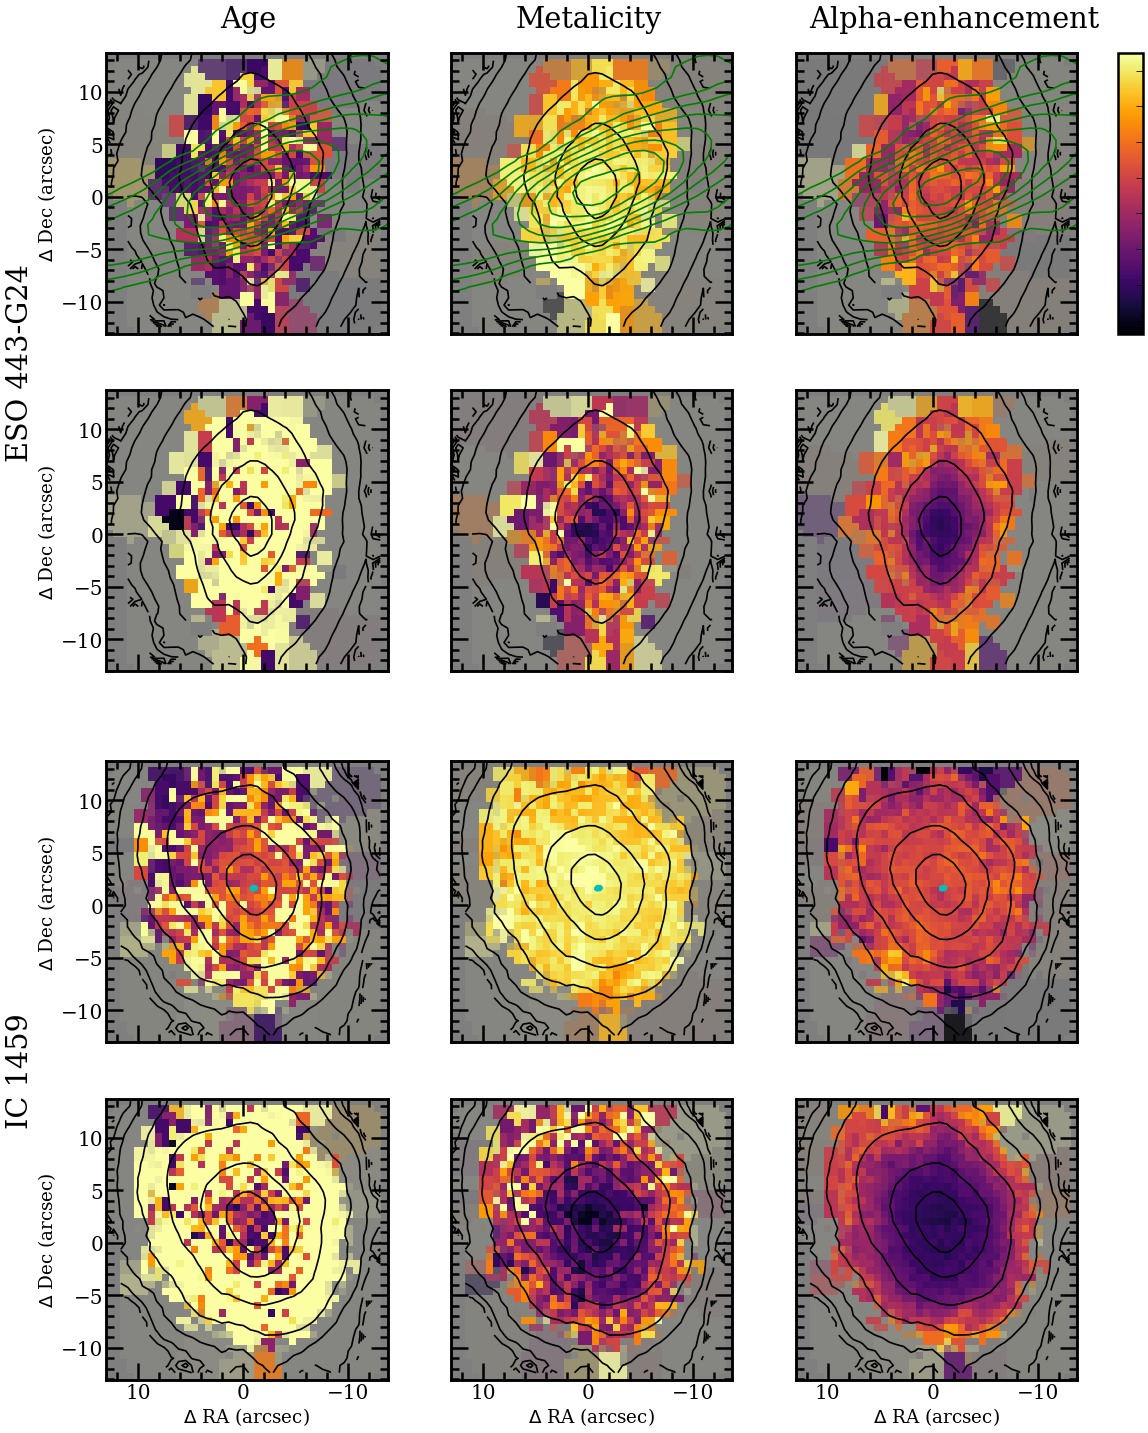
\includegraphics[height=0.94\textheight]{chapter4/vimos/pop1.png}
			\caption[VIMOS stellar population maps]{VIMOS stellar population maps: From left to right: age, metallicity and alpha enhancement, Top to bottom ESO 443-G24, IC 1459 and IC 1531. Rows show parameter and uncertainty in the parameter on alternate rows. Plots are as in figure \ref{fig:VIMOS_stellar}. Color scales have limits reflecting the range of SSP available models.}
			\label{fig:VIMOS_pop}
		\end{figure}
		\begin{figure}
			\centering
			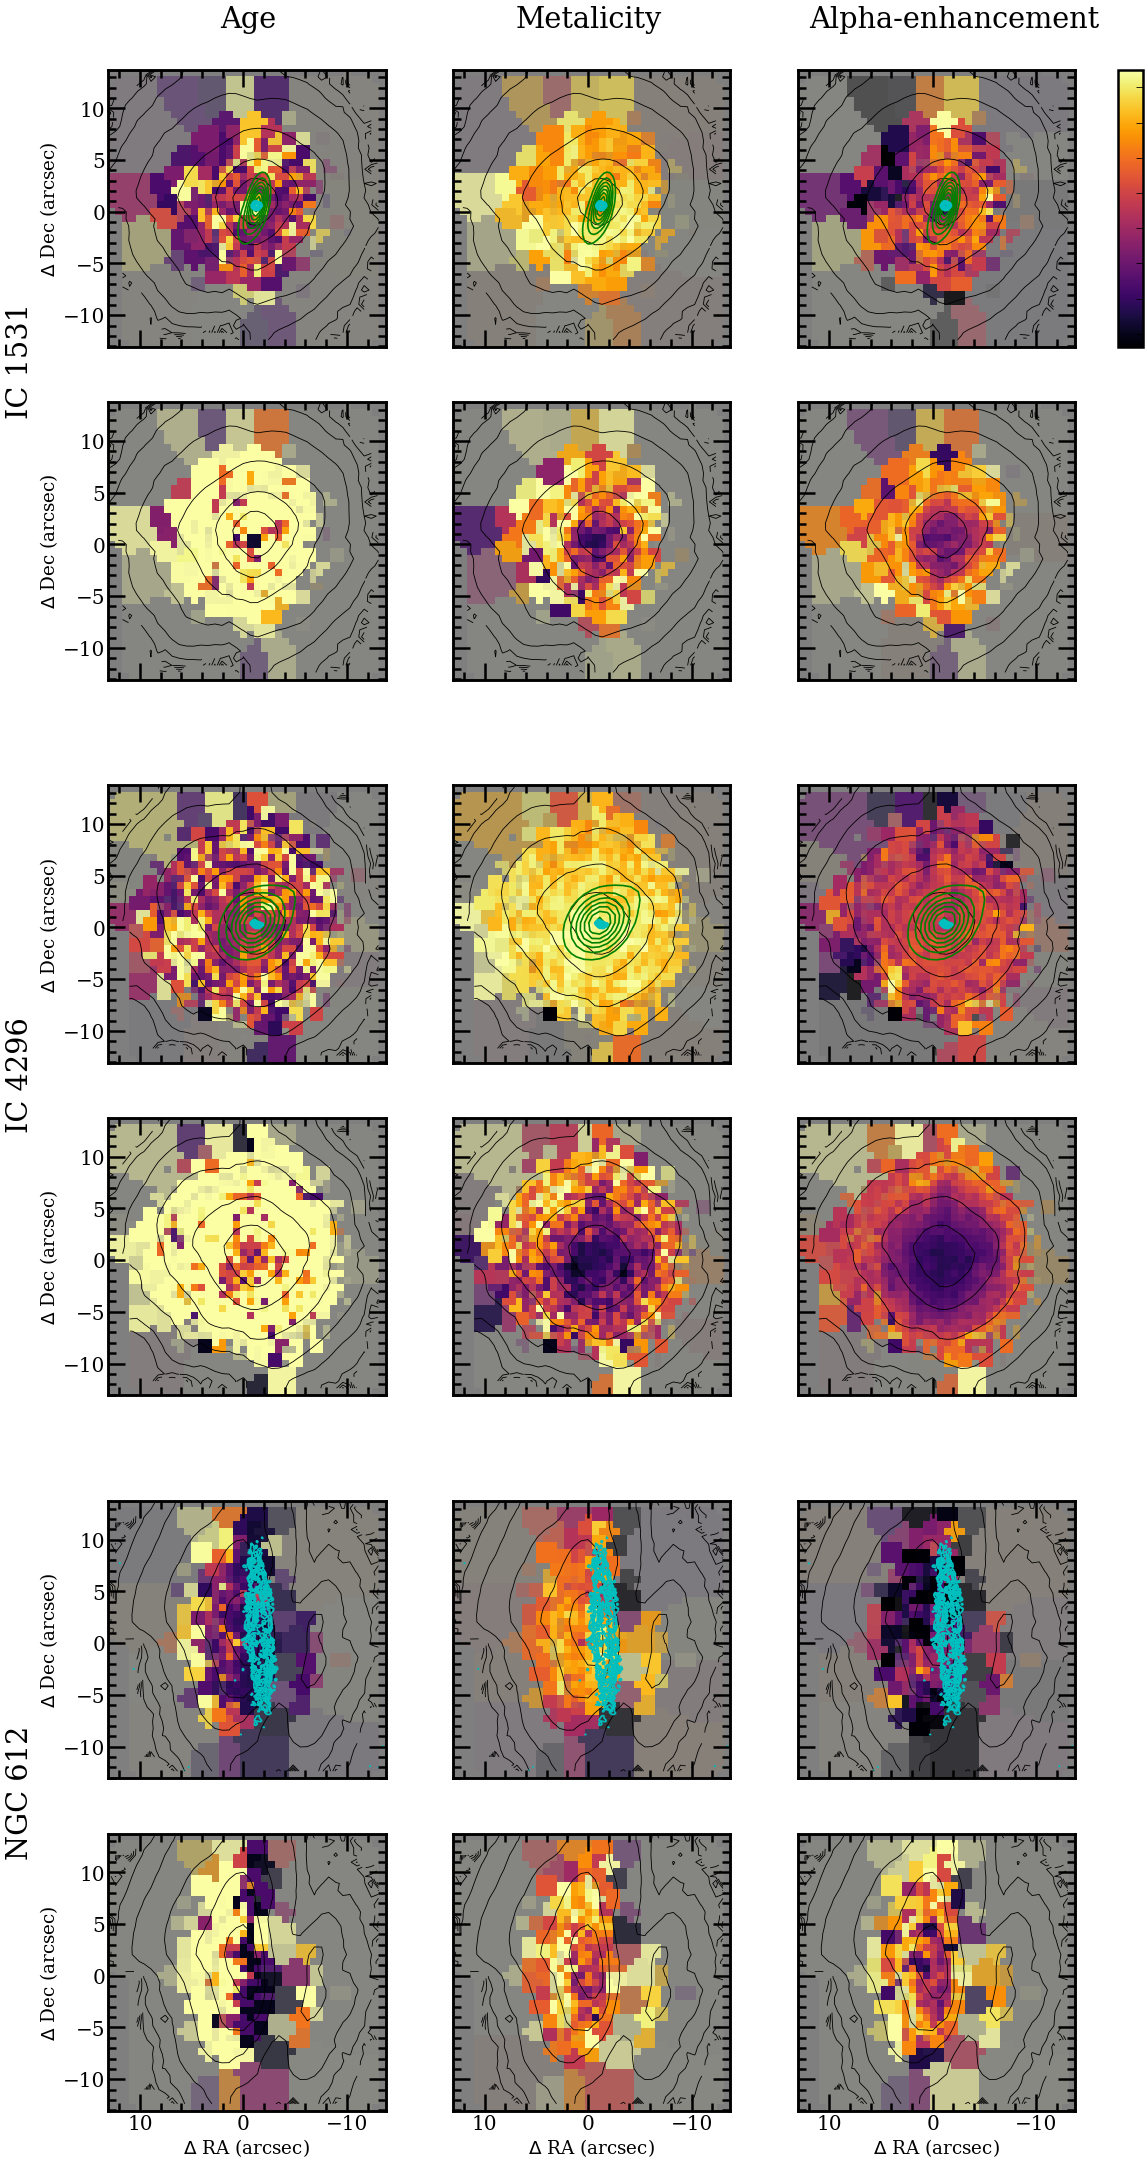
\includegraphics[height=0.94\textheight]{chapter4/vimos/pop2.png}
			\contcaption{continued for IC 4296, NGC 612 and NGC 1399}
		\end{figure}
		\begin{figure}
			\centering
			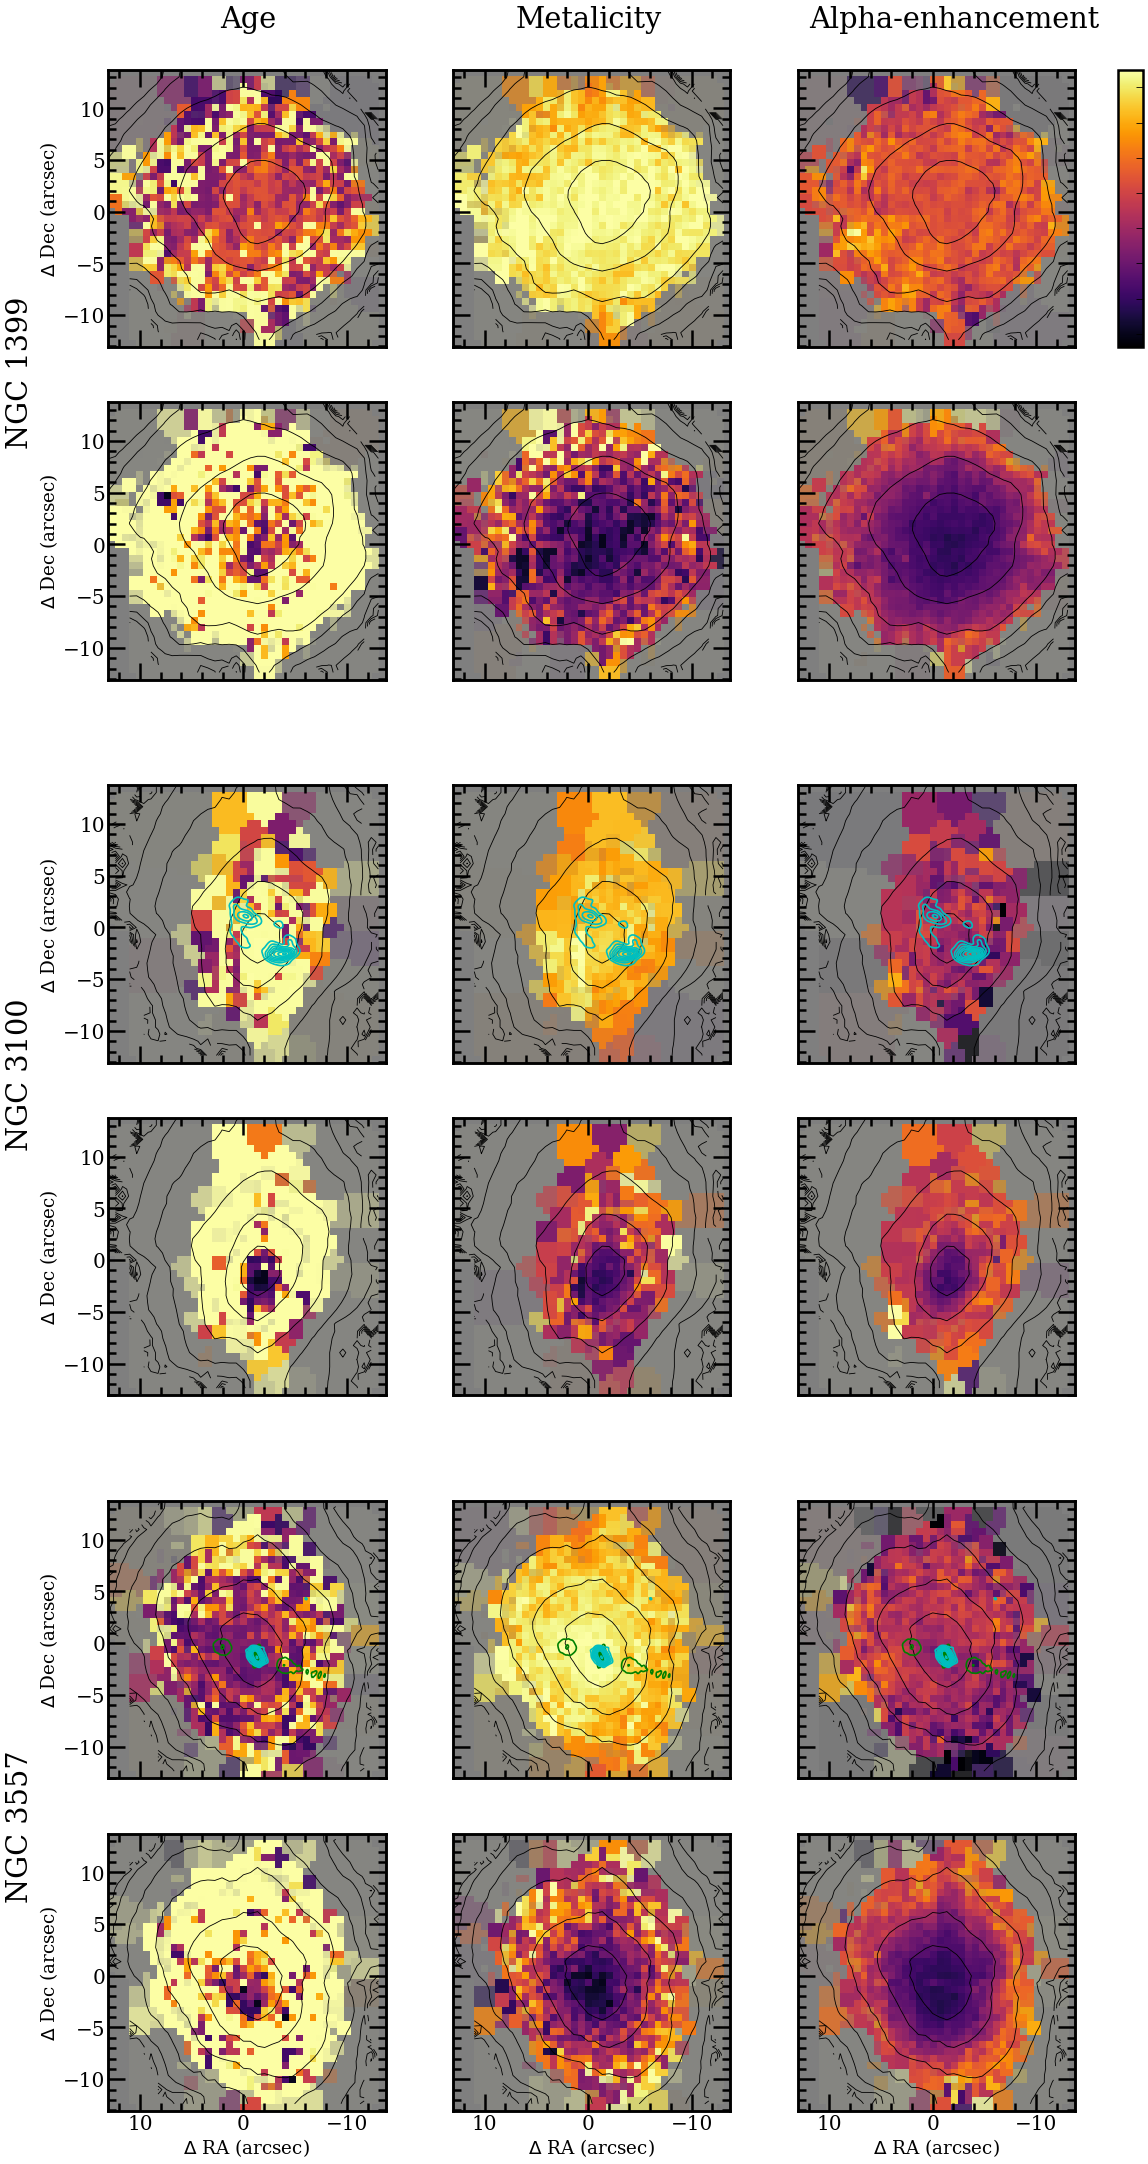
\includegraphics[height=0.94\textheight]{chapter4/vimos/pop3.png}
			\contcaption{continued for NGC 3100, NGC 3557 and NGC 7075}
		\end{figure}
		\begin{figure}
			\centering
			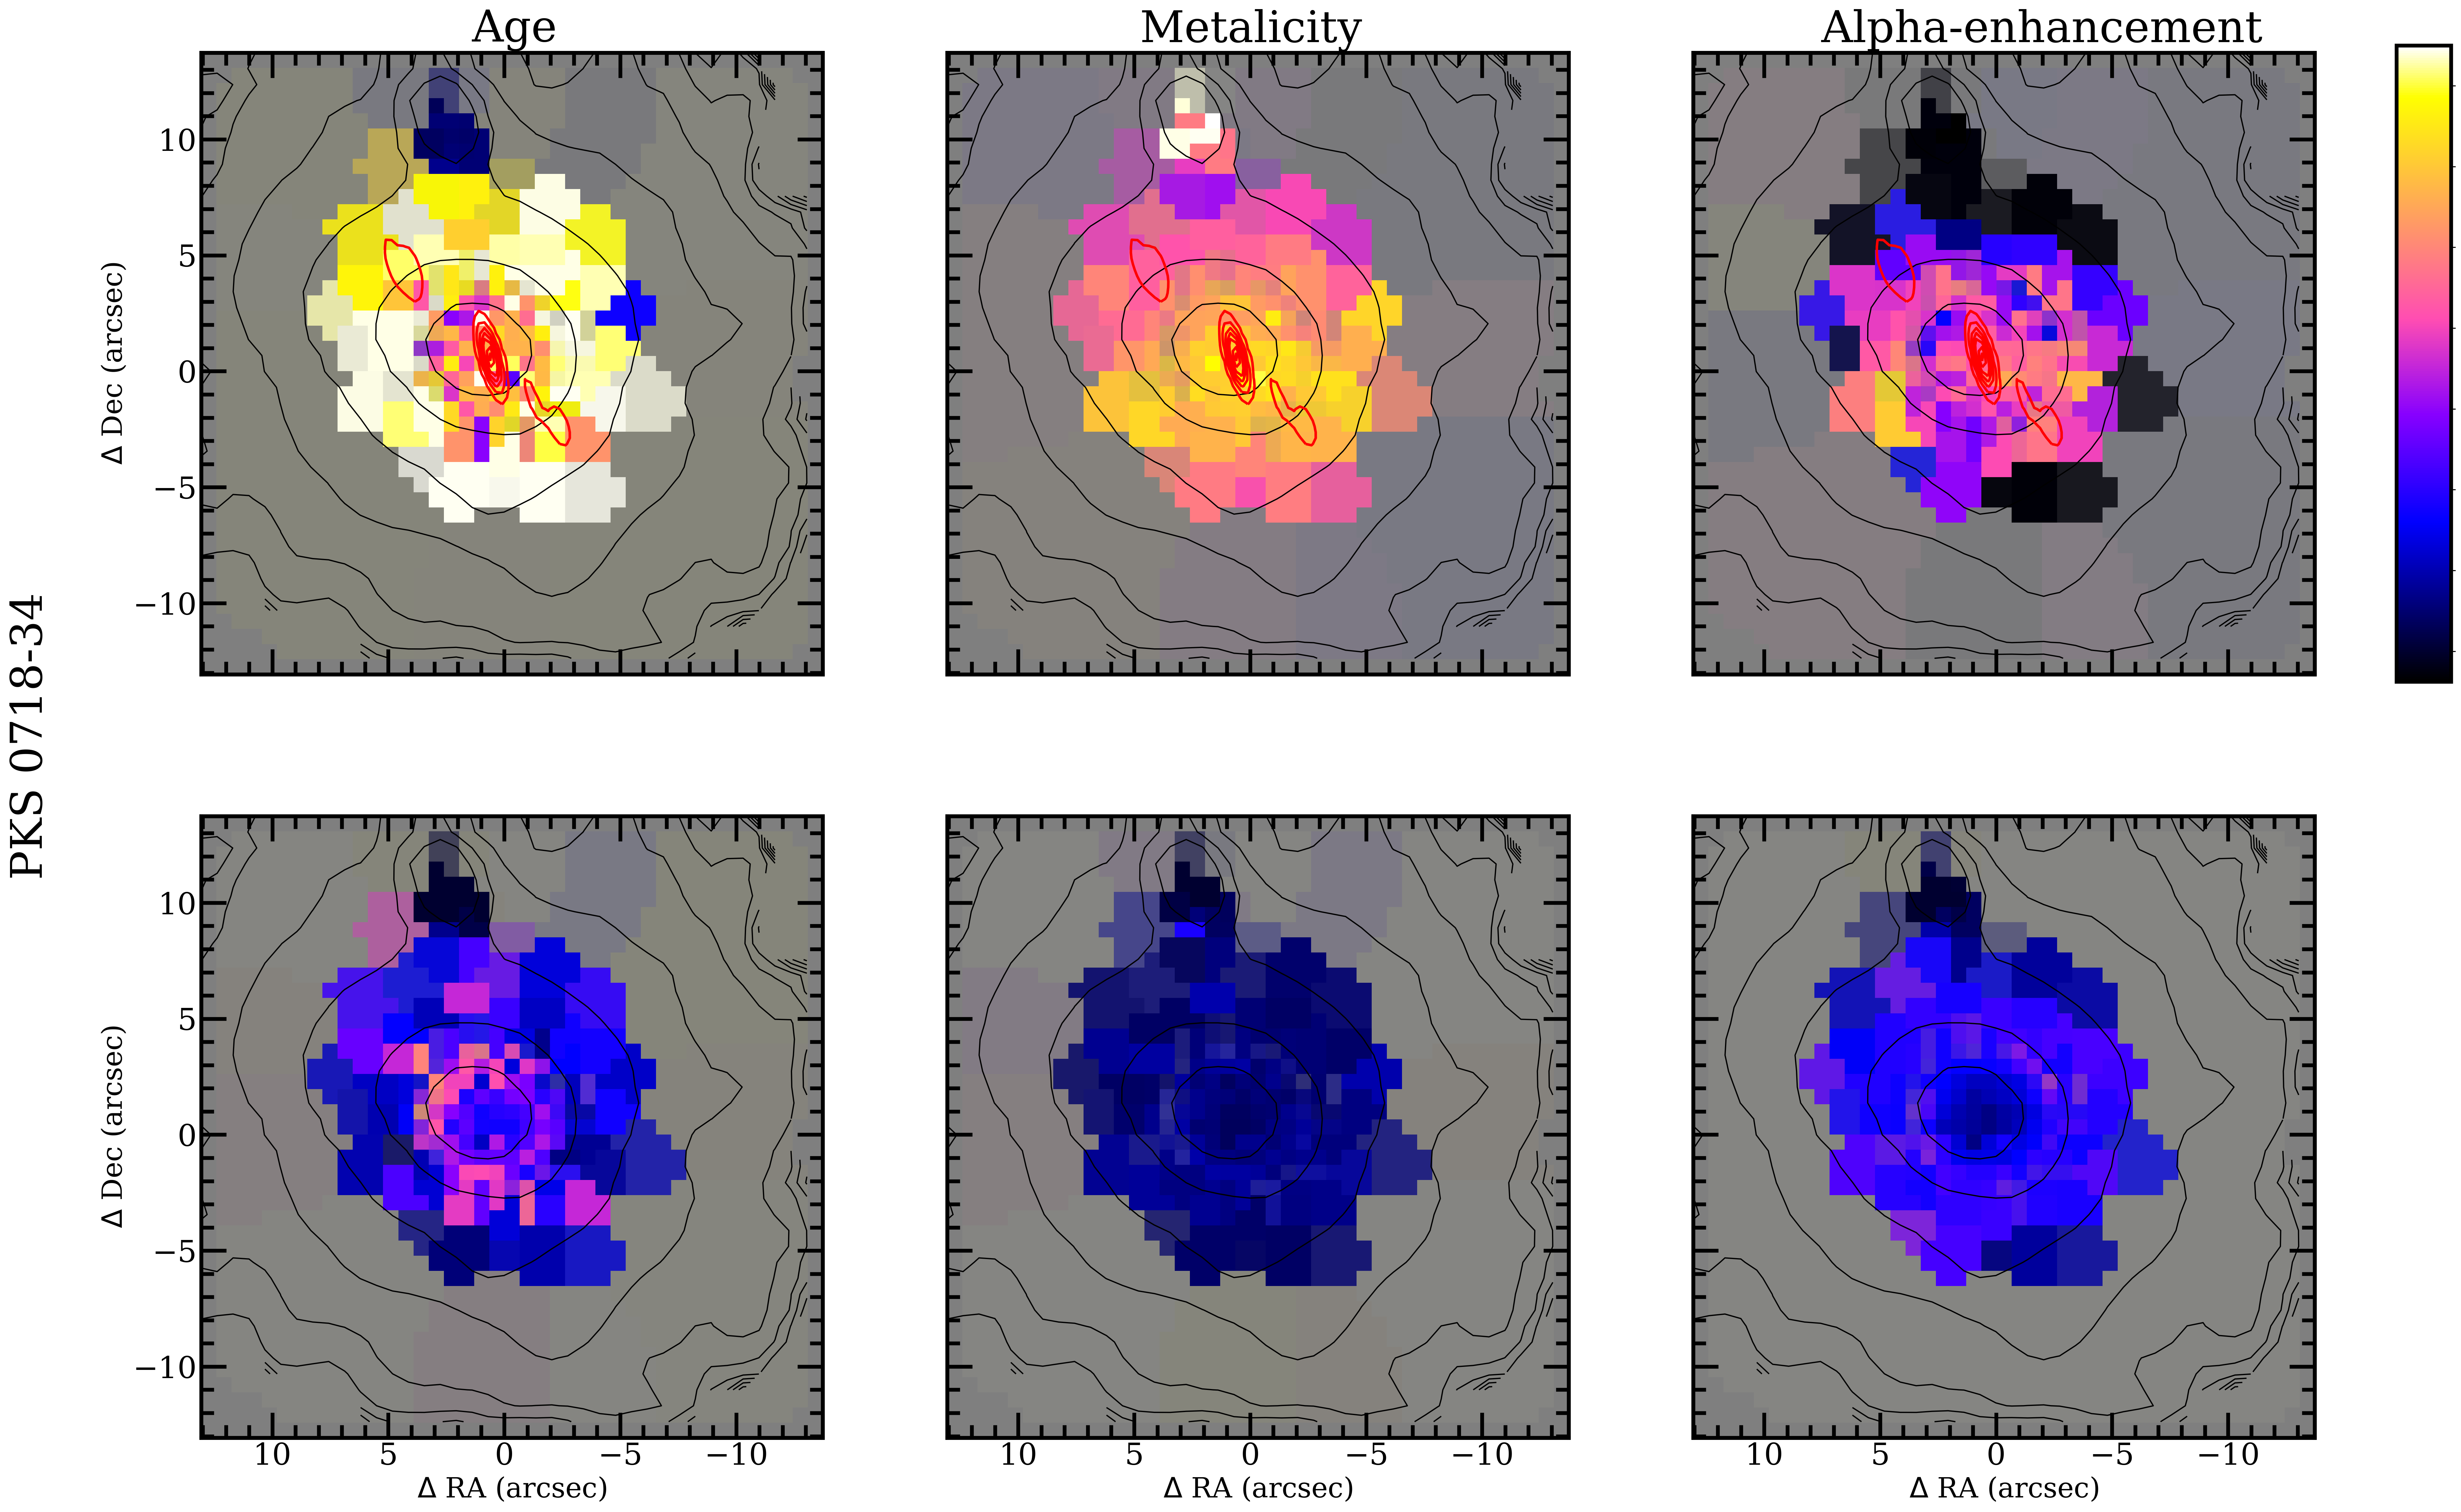
\includegraphics[height=0.31\textheight]{chapter4/vimos/pop4.png}
			\contcaption{continued for PKS 718-34}
		\end{figure}

		\begin{figure}
			\centering
			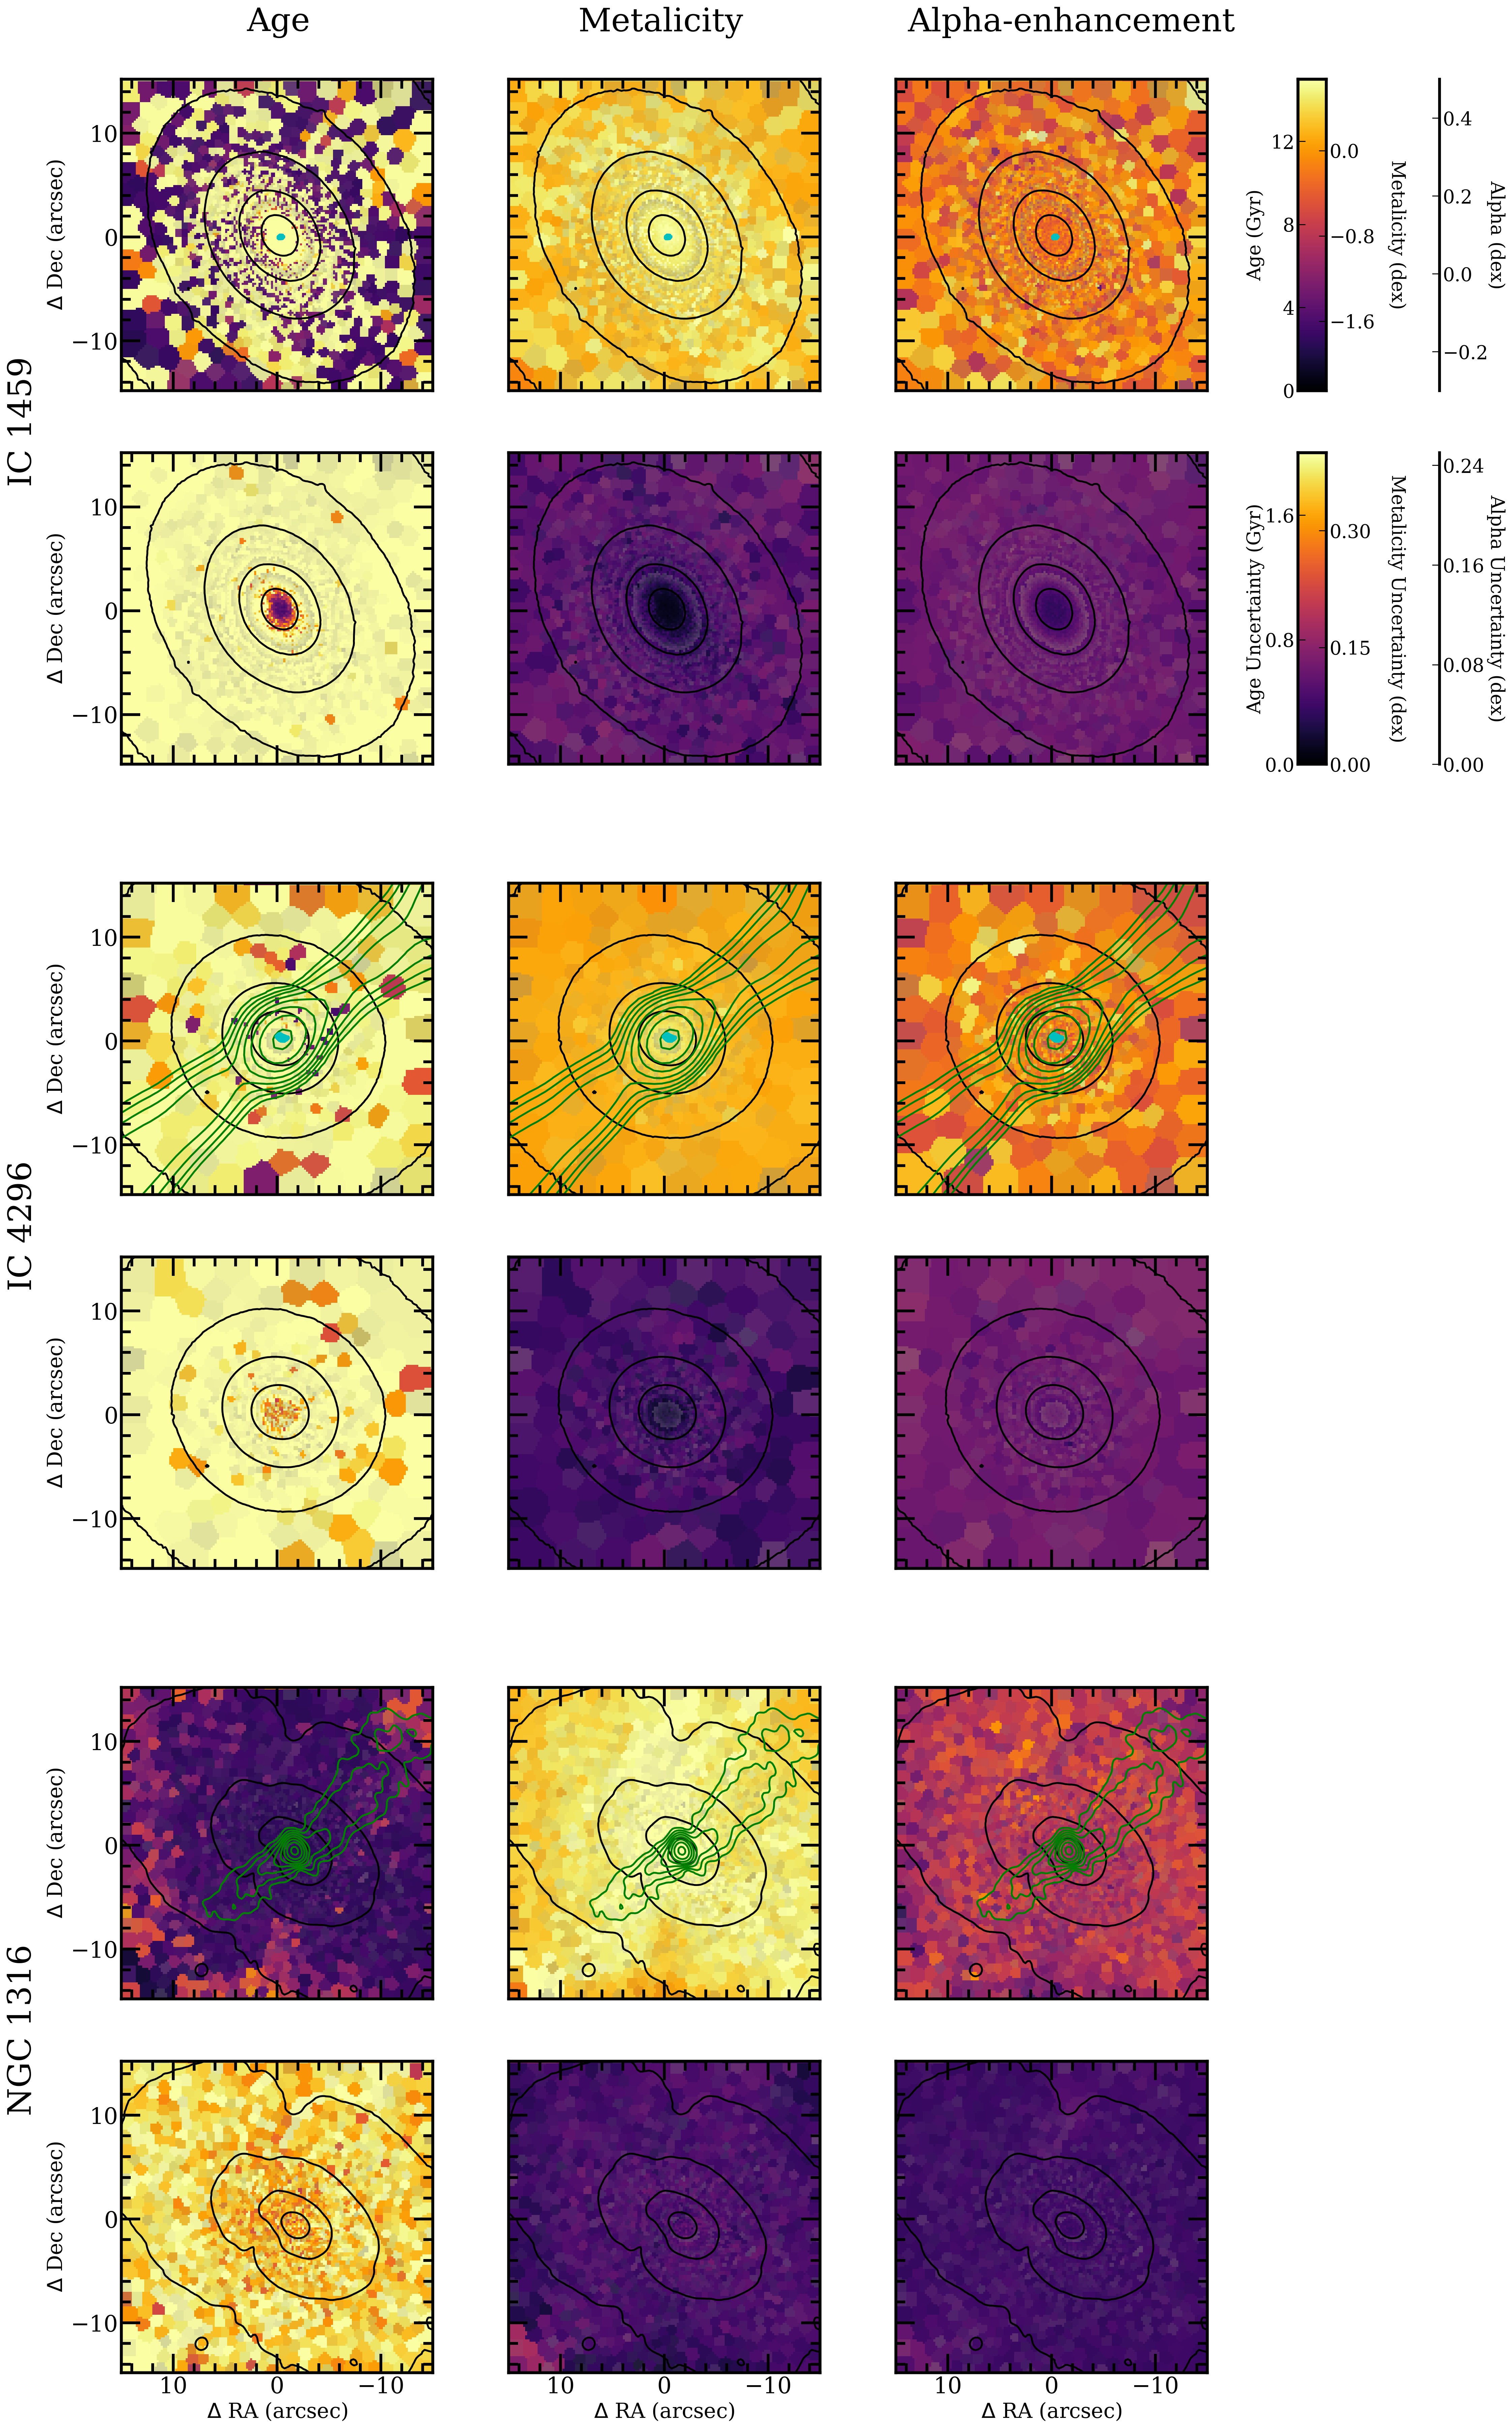
\includegraphics[height=0.94\textheight]{chapter4/muse/pop1.png}
			\caption[MUSE stellar population maps]{MUSE stellar population maps: From top to bottom IC 1459, IC 4296 and NGC 1316. Plots are as in figure \ref{fig:VIMOS_stellar}. Color scales have limits reflecting the range of SSP available models.}
			\label{fig:MUSE_pop}
		\end{figure}
		\begin{figure}
			\centering
			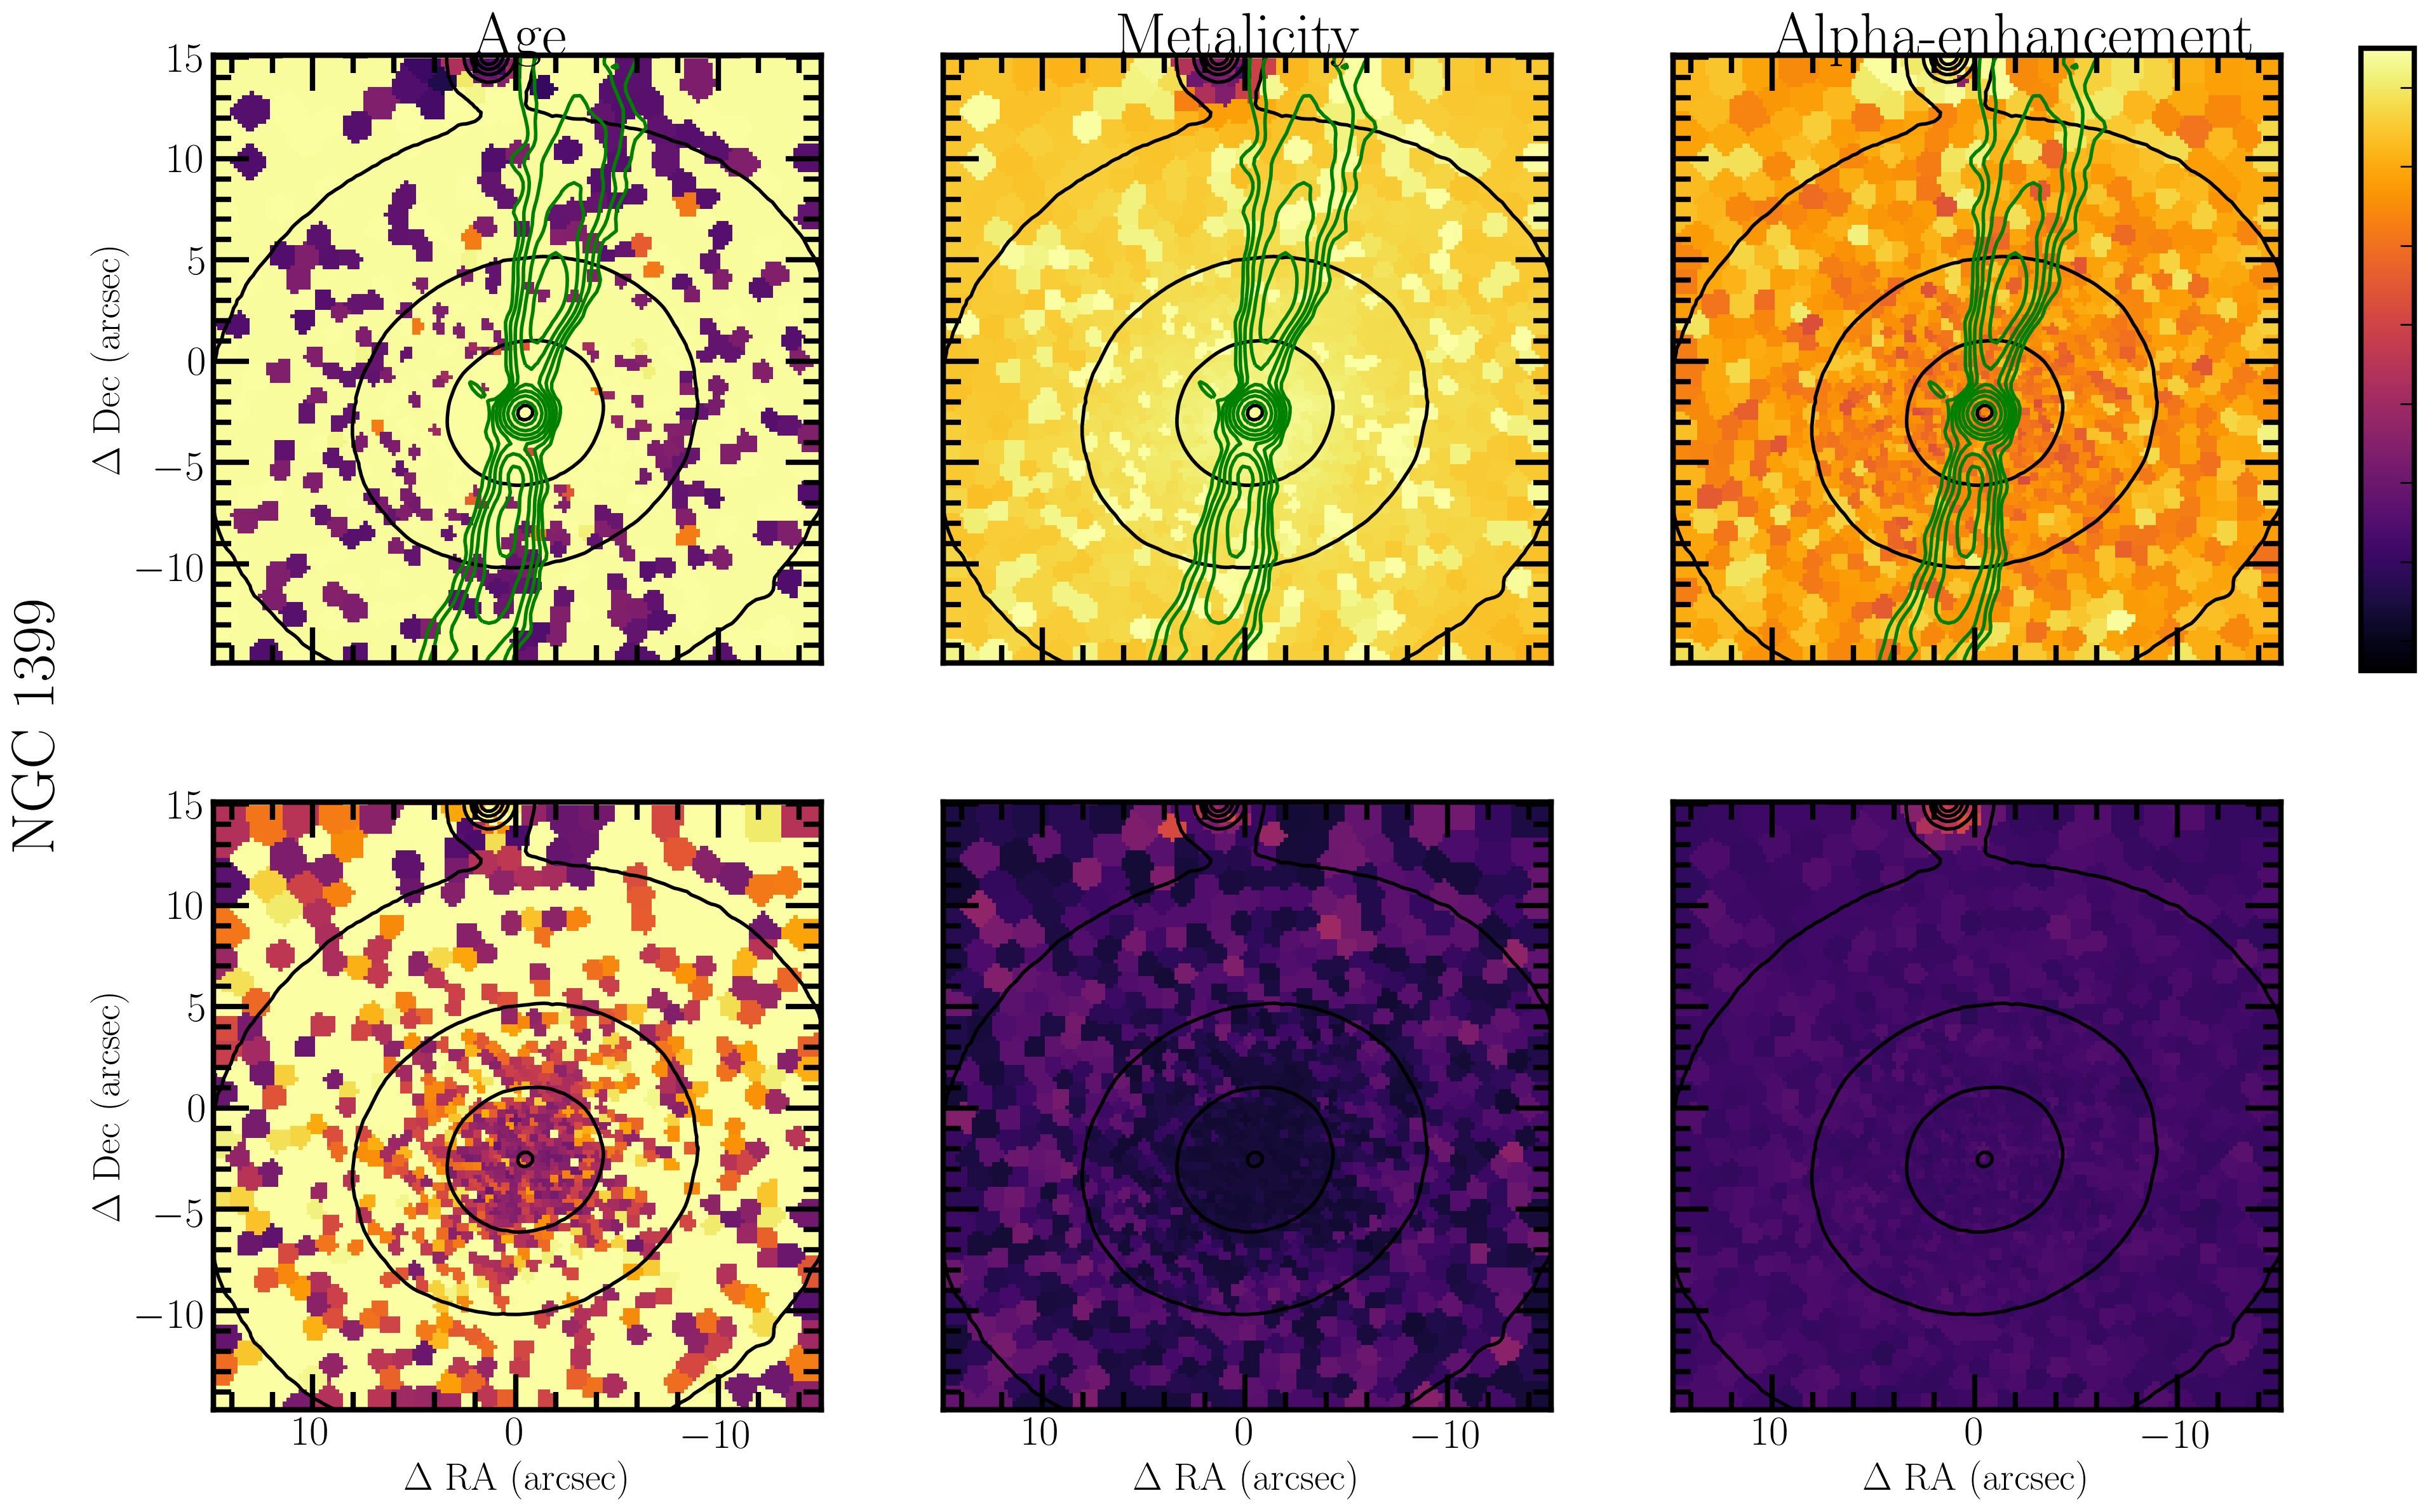
\includegraphics[height=0.31\textheight]{chapter4/muse/pop2.png}
			\contcaption{continued for NGC 1399}
		\end{figure}


		\subsubsection{Radial Gradients in Stellar Populations}
			\label{subsubsec:popGrad}

			\citet{Koleva2011} showed that while there can be a large spread in radial gradients of age and metallicity, the mean is fairly well confined. They assume a linear relationship between $\log t$ or $[Fe/H]$ and $\log (R/\mathrm{R_e})$. The distance from the center of the galaxy to a given point is $R$ and $\mathrm{R_e}$ is the effective radius: the radius which contains which half of the total light emitted by the galaxy. For elliptical galaxies they find average gradients of $0.06\pm0.09 \, \mathrm{log(Gyr) \, arcsec^{-1}}$ and $-0.26\pm0.08 \, \mathrm{[Fe/H]_\odot \, arcsec^{-1}}$ for the age and metallicity gradients respectively. For S0s they find flatter corresponding gradients of $0.01\pm0.11$ and $-012\pm0.13$. The results from our southern sample are shown in table \ref{tab:popGrad}. We find average gradients of $\Delta_\text{log age} = -0.004\pm0.003 \,\mathrm{log(Gyr) \, arcsec^{-1}}$ and $\Delta_\text{[Fe/H]} = -0.025\pm0.002 \mathrm{[Fe/H]_\odot \, arcsec^{-1}}$, which is consistent with \citet{Koleva2011}.

			\begin{table}
				\centering
				\caption{The radial gradients of the most-likely SSP models.}
				\label{tab:popGrad}
				\begin{tabular}{l c c}
					\hline
					\hline 
					Galaxy 	& $\Delta_\text{log age}$ & $\Delta_\text{[Fe/H]}$ \\ 
						& log(Gyr) arcsec$^{-1}$ & [Fe/H]$_\odot$ arcsec$^{-1}$ \\
					\hline
					ESO 443-G024 & $-0.008 \pm 0.006$ & $-0.028 \pm 0.005$ \\
					IC 1459 	& $-0.024 \pm 0.011$ & $-0.024 \pm 0.022$ \\
					IC 1531 	& $-0.016 \pm 0.006$ & $0.004 \pm 0.009$ \\
					IC 4296		& $0.001 \pm 0.001$ & $0.071 \pm 0.006$ \\
					NGC 612 	& $0.021 \pm 0.024$ & $-0.101 \pm 0.012$ \\
					NGC 1316 	& $0.007 \pm 0.004$ & $0.005 \pm 0.006$ \\
					NGC 1399 	& $-0.035 \pm 0.008$ & $0.041 \pm 0.006$ \\
					NGC 3100 	& $0.000 \pm 0.004$ & $-0.045 \pm 0.003$ \\
					NGC 3557 	& $0.000 \pm 0.006$ & $-0.023 \pm 0.007$ \\
					NGC 7075 	& $0.006 \pm 0.003$ & $-0.067 \pm 0.006$ \\
					PKS 718-34  & $0.008 \pm 0.007$ & $-0.115 \pm 0.007$ \\
					\hline
					\hline
				\end{tabular}
			\end{table}



	\subsection{Kinematically Decoupled Cores}
		\label{subsec:popKDC}

		\citet{Kuntschner2010} found that kinematically decoupled cores (KDCs) exist in two forms: they are either small or contain an old stellar population. The two definite KDCs found in the Southern Sample fit into this pattern: both have old stellar populations and large sizes. It is worth noting that in many cases we would not spatially resolve a small KDCs with VIMOS data. Figure \ref{fig:KDC} shows the KDC size -- age relation including the Southern Sample. KDC size is the radius at which $k_1$ (defined in section \ref{sec:ETG}) reaches zero at the boundary between inner and outer components. Age is found from finding the most-likely SSP model for the spatially integrated spectrum within the a radius of 1 arcsec about the center of the galaxy. We have included PKS 718-34 in this plot but stress it is only tentatively classified as containing a KDC from the kinematics from VIMOS. Figure \ref{fig:KDC} shows that while PKS 718-34 would be an extremely large KDC it still is consistent with the findings of \citet{Kuntschner2010}.

		\begin{figure}
			\centering
			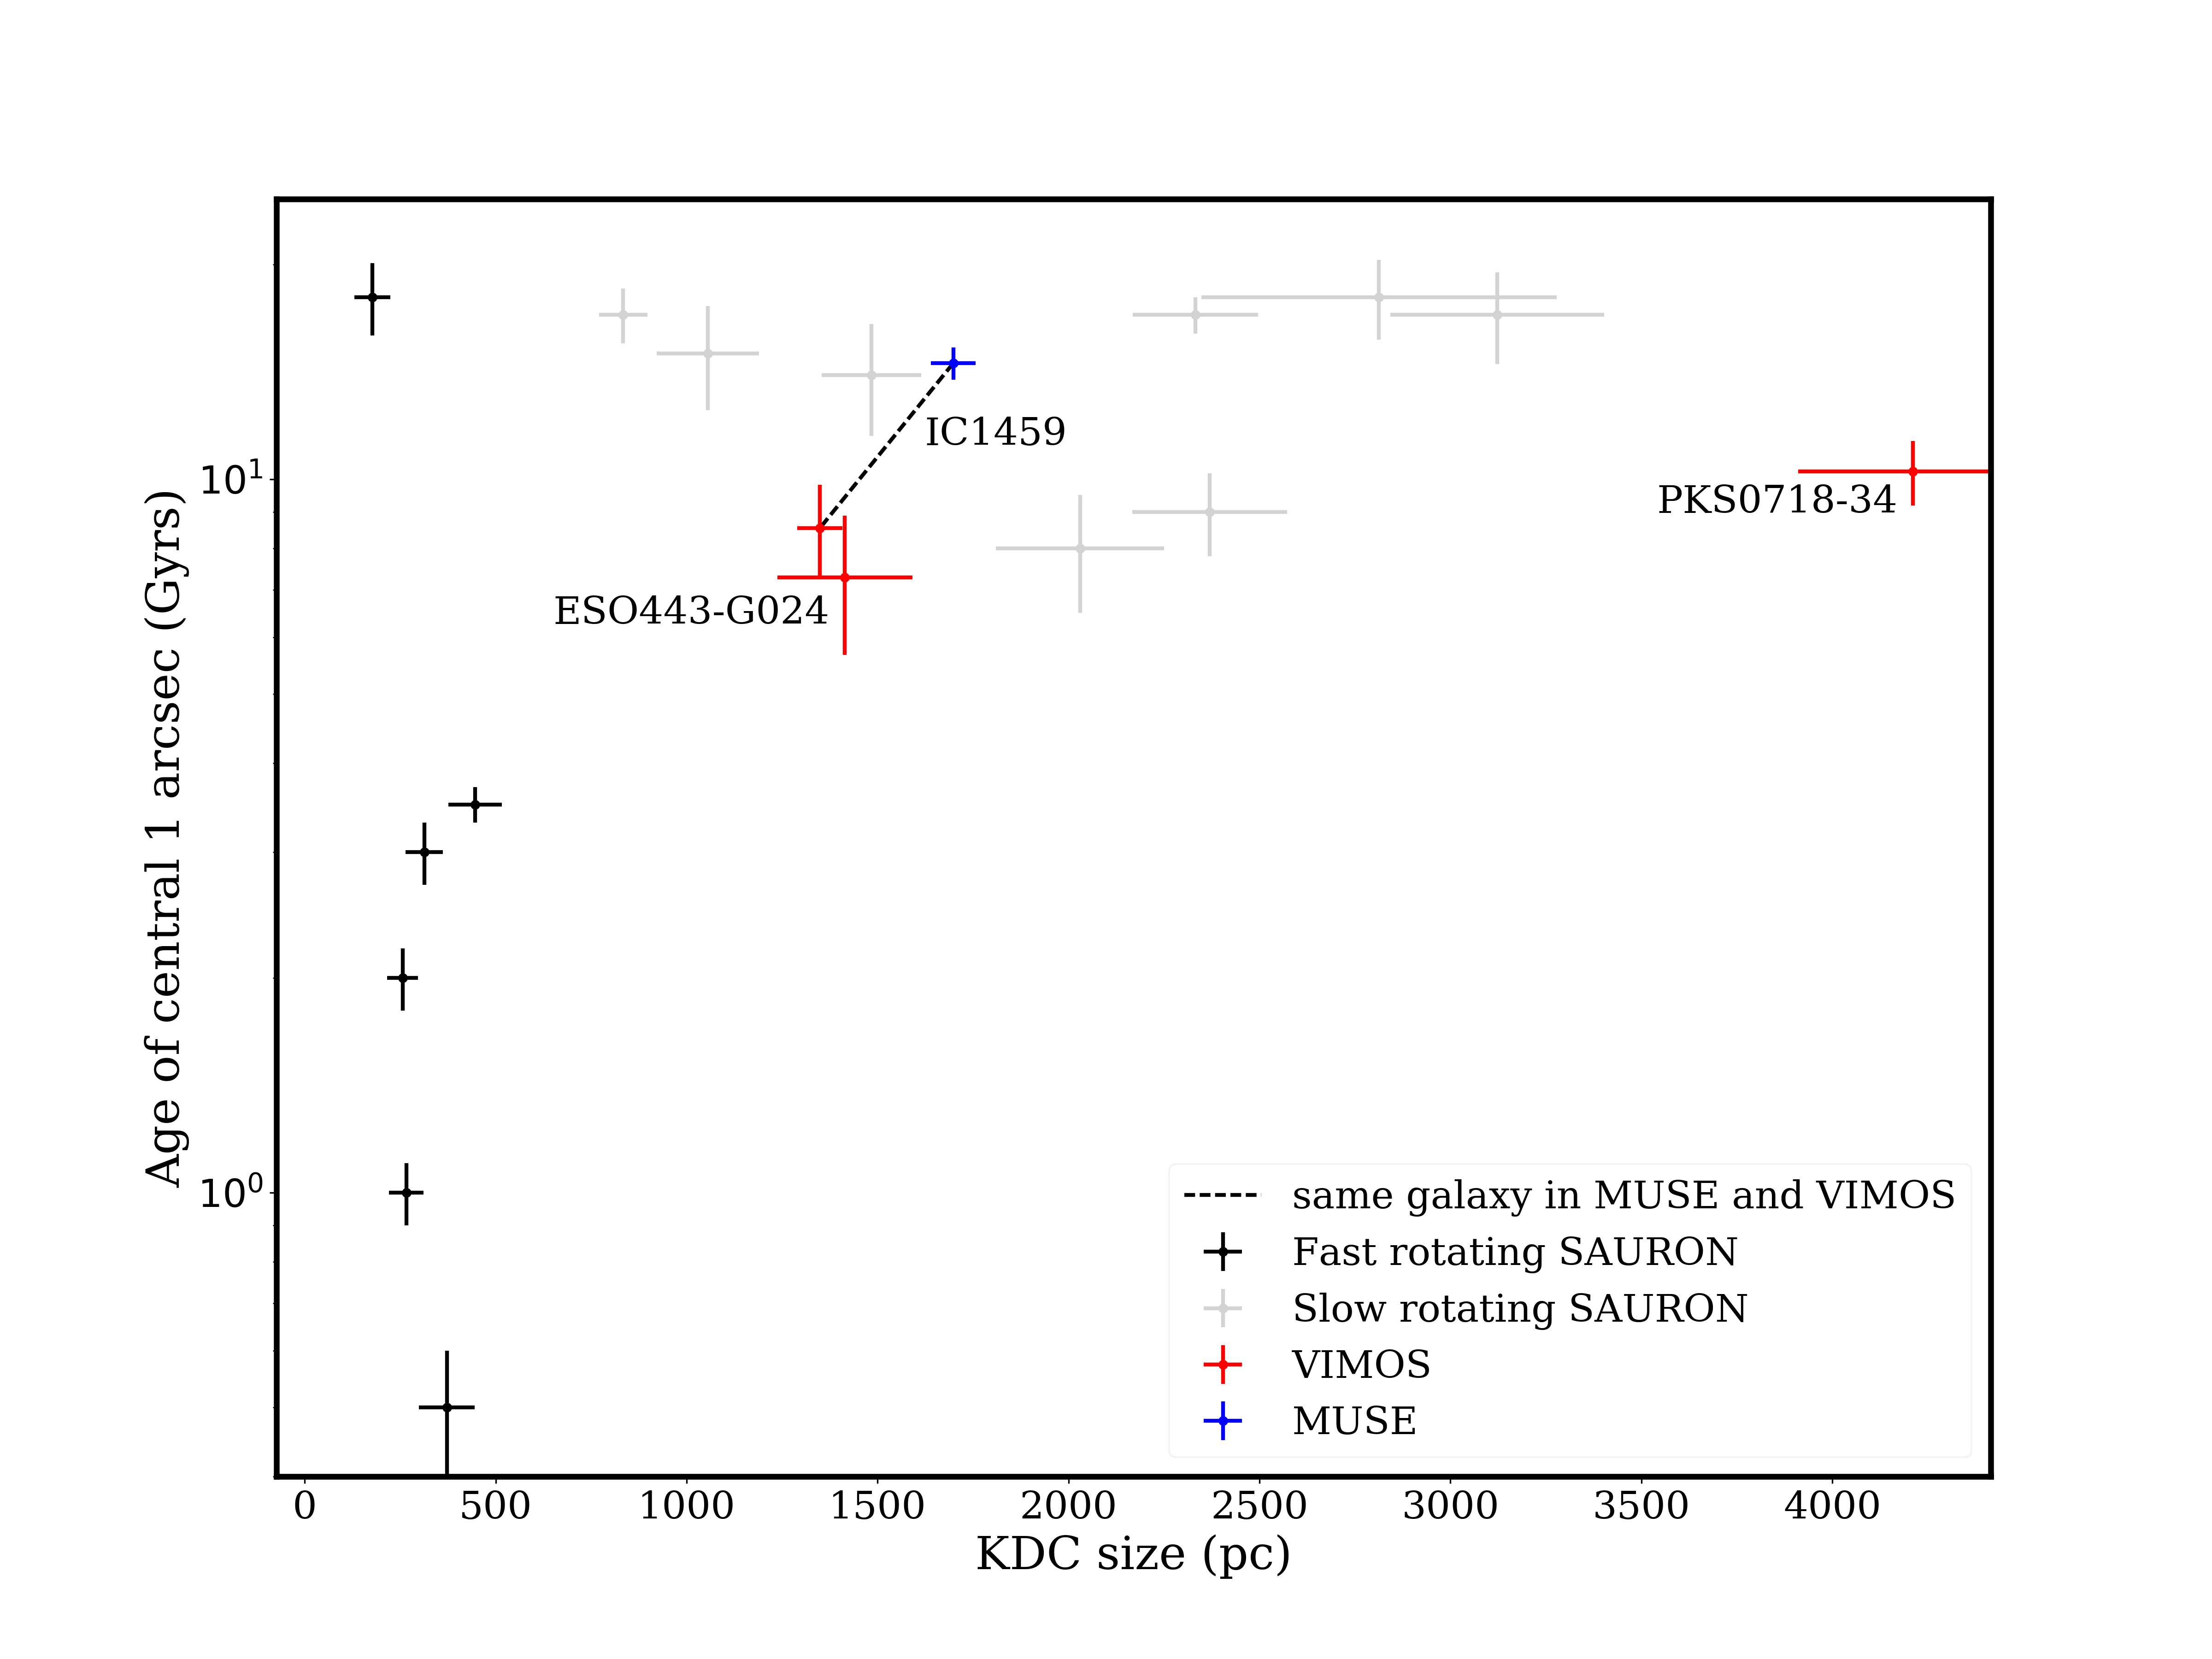
\includegraphics[width=.7\textwidth]{chapter4/KDC_size_age.png}
			\caption[KDC dichotomy]{The KDC size -- age relation showing KDCs are either old or small. Colors of symbols are: VIMOS in red, MUSE in blue and SAURON from \citet{Kuntschner2010} in black and gray for fast and slow rotators respectively (Atlas$^\text{3D}$ did not repeat these measurements after SAURON.}
			\label{fig:KDC}
		\end{figure}


	\subsection{Mg -- $\sigma$ relation}
		\label{subsec:Mgsigma}

		It was \citet{Bender1993} who first noticed the unusually tight relationship between the global Mg absorption line strength and velocity dispersion for elliptical galaxies. They also noticed that residuals appeared to be intrinsic as they had a near Gaussian shape about the median values, but did not seem to be correlated to any other galaxy property. Since there is no known process that would correlate these values at late times in the evolution of galaxy, the notion that ETGs have a very short formation epoch at high redshift is favoured. 

		\citet{Mehlert2003} showed the existence of the internal Mg--$\mathrm{\sigma}$ relation, but also suggested that it had a different origin to that of the global relation. They found that alpha-enhancement correlates with velocity dispersion and drives about 30\% of the global Mg--$\sigma$ relation. Metallicity variations provide the remaining 70\%. The alpha-enhancement usually has no radial gradient (while velocity dispersion is highly dependent on radius) suggesting that alpha-enhancement has no role in the internal Mg--$\sigma$ relation. 

		\subsubsection{Global Relation}
			Using an aperture with a radius of 2 arcsec on each dataset, we find a global linear gradient of $2.7\pm1.9 \,\mathrm{\AA/\log(km \, s^{-1})}$. This is consistent with the gradient found by \citet{Ziegler1997} for a sample of elliptical galaxies within Virgo and Coma using data from \citet{Dressler1987}. However, figure \ref{fig:globalMg} shows there is a considerable offset of $\approx0.75\,\mathrm{\AA}$ between our best-fitting line (solid line) and the best-fitting line (dashed line) from \citet{Ziegler1997}. Individual measurements for each galaxy are given in table \ref{tab:globalMg}.
			%%no uncertainties quoted in Dressler1987 so comparison is meaningless.
			%NGC 1399 was observed by \citet{Dressler1987}, but measures Mg$_2$ instead of Mg$_b$. In order to compare we make use of the linear conversion (eq. 1 in \citet{Ziegler1997}):
			% \begin{equation}
			% 	\mathrm{Mg_b \, \AA^{-1}} = 15 \mathrm{Mg_2 \, mag^{-1}}
			% \end{equation}
			% Using this gives that \citet{Dressler1987} measured NGC 1399 to have a Mg$_b$ strength of 5.175 and a velocity dispersion of 299.9 km s$^{-1}$, however \citet{Dressler1987} does not quote uncertainties for their values so it is difficult to make comparisons. 

			\begin{table}
				\centering
			\begin{threeparttable}
				\caption{The Mg$_b$ index and velocity dispersion within 2 arcsec.}
				\label{tab:globalMg}
				\begin{tabular}{l c c}
					\hline
					\hline
					Galaxy 	& Mg$_b$ & $\sigma$ \\
							& \AA 	& km s$^{-1}$ \\
					\hline
					ESO 443-G024 & $4.43 \pm 0.08$ & $332.4 \pm 1.6$ \\
					IC 1459 	& $4.67 \pm 0.03$ & $292.7 \pm 0.6$ \\
					IC 1531 	& $3.74 \pm 0.06$ & $222.9 \pm 1.3$ \\
					IC 4296		& $4.57 \pm 0.13$ & $361.7 \pm 2.1$ \\
					NGC 612 	& --   			  & $228.5 \pm 1.9$ \\
					NGC 1316 	& $3.45 \pm 0.08$ & $233.3 \pm 1.5$ \\
					NGC 1399 	& $4.57 \pm 0.13$ & $319.1 \pm 2.1$ \\
					NGC 3100 	& $4.36 \pm 0.05$ & $214.2 \pm 1.1$ \\
					NGC 3557 	& $4.15 \pm 0.03$ & $280.4 \pm 0.9$ \\
					NGC 7075 	& $4.45 \pm 0.07$ & $258.7 \pm 1.9$ \\
					PKS 718-34  & -- 		      & $258.7 \pm 1.9$ \\
					\hline
					\hline
				\end{tabular}
				\begin{tablenotes}
				\footnotesize
				\item NGC 612 and PKS 718-34 have a redshift which shifts the Mg$_b$ feature outside of the wavelength range of VIMOS.
				\end{tablenotes}
			\end{threeparttable}
			\end{table}

			\begin{figure}
				\centering
				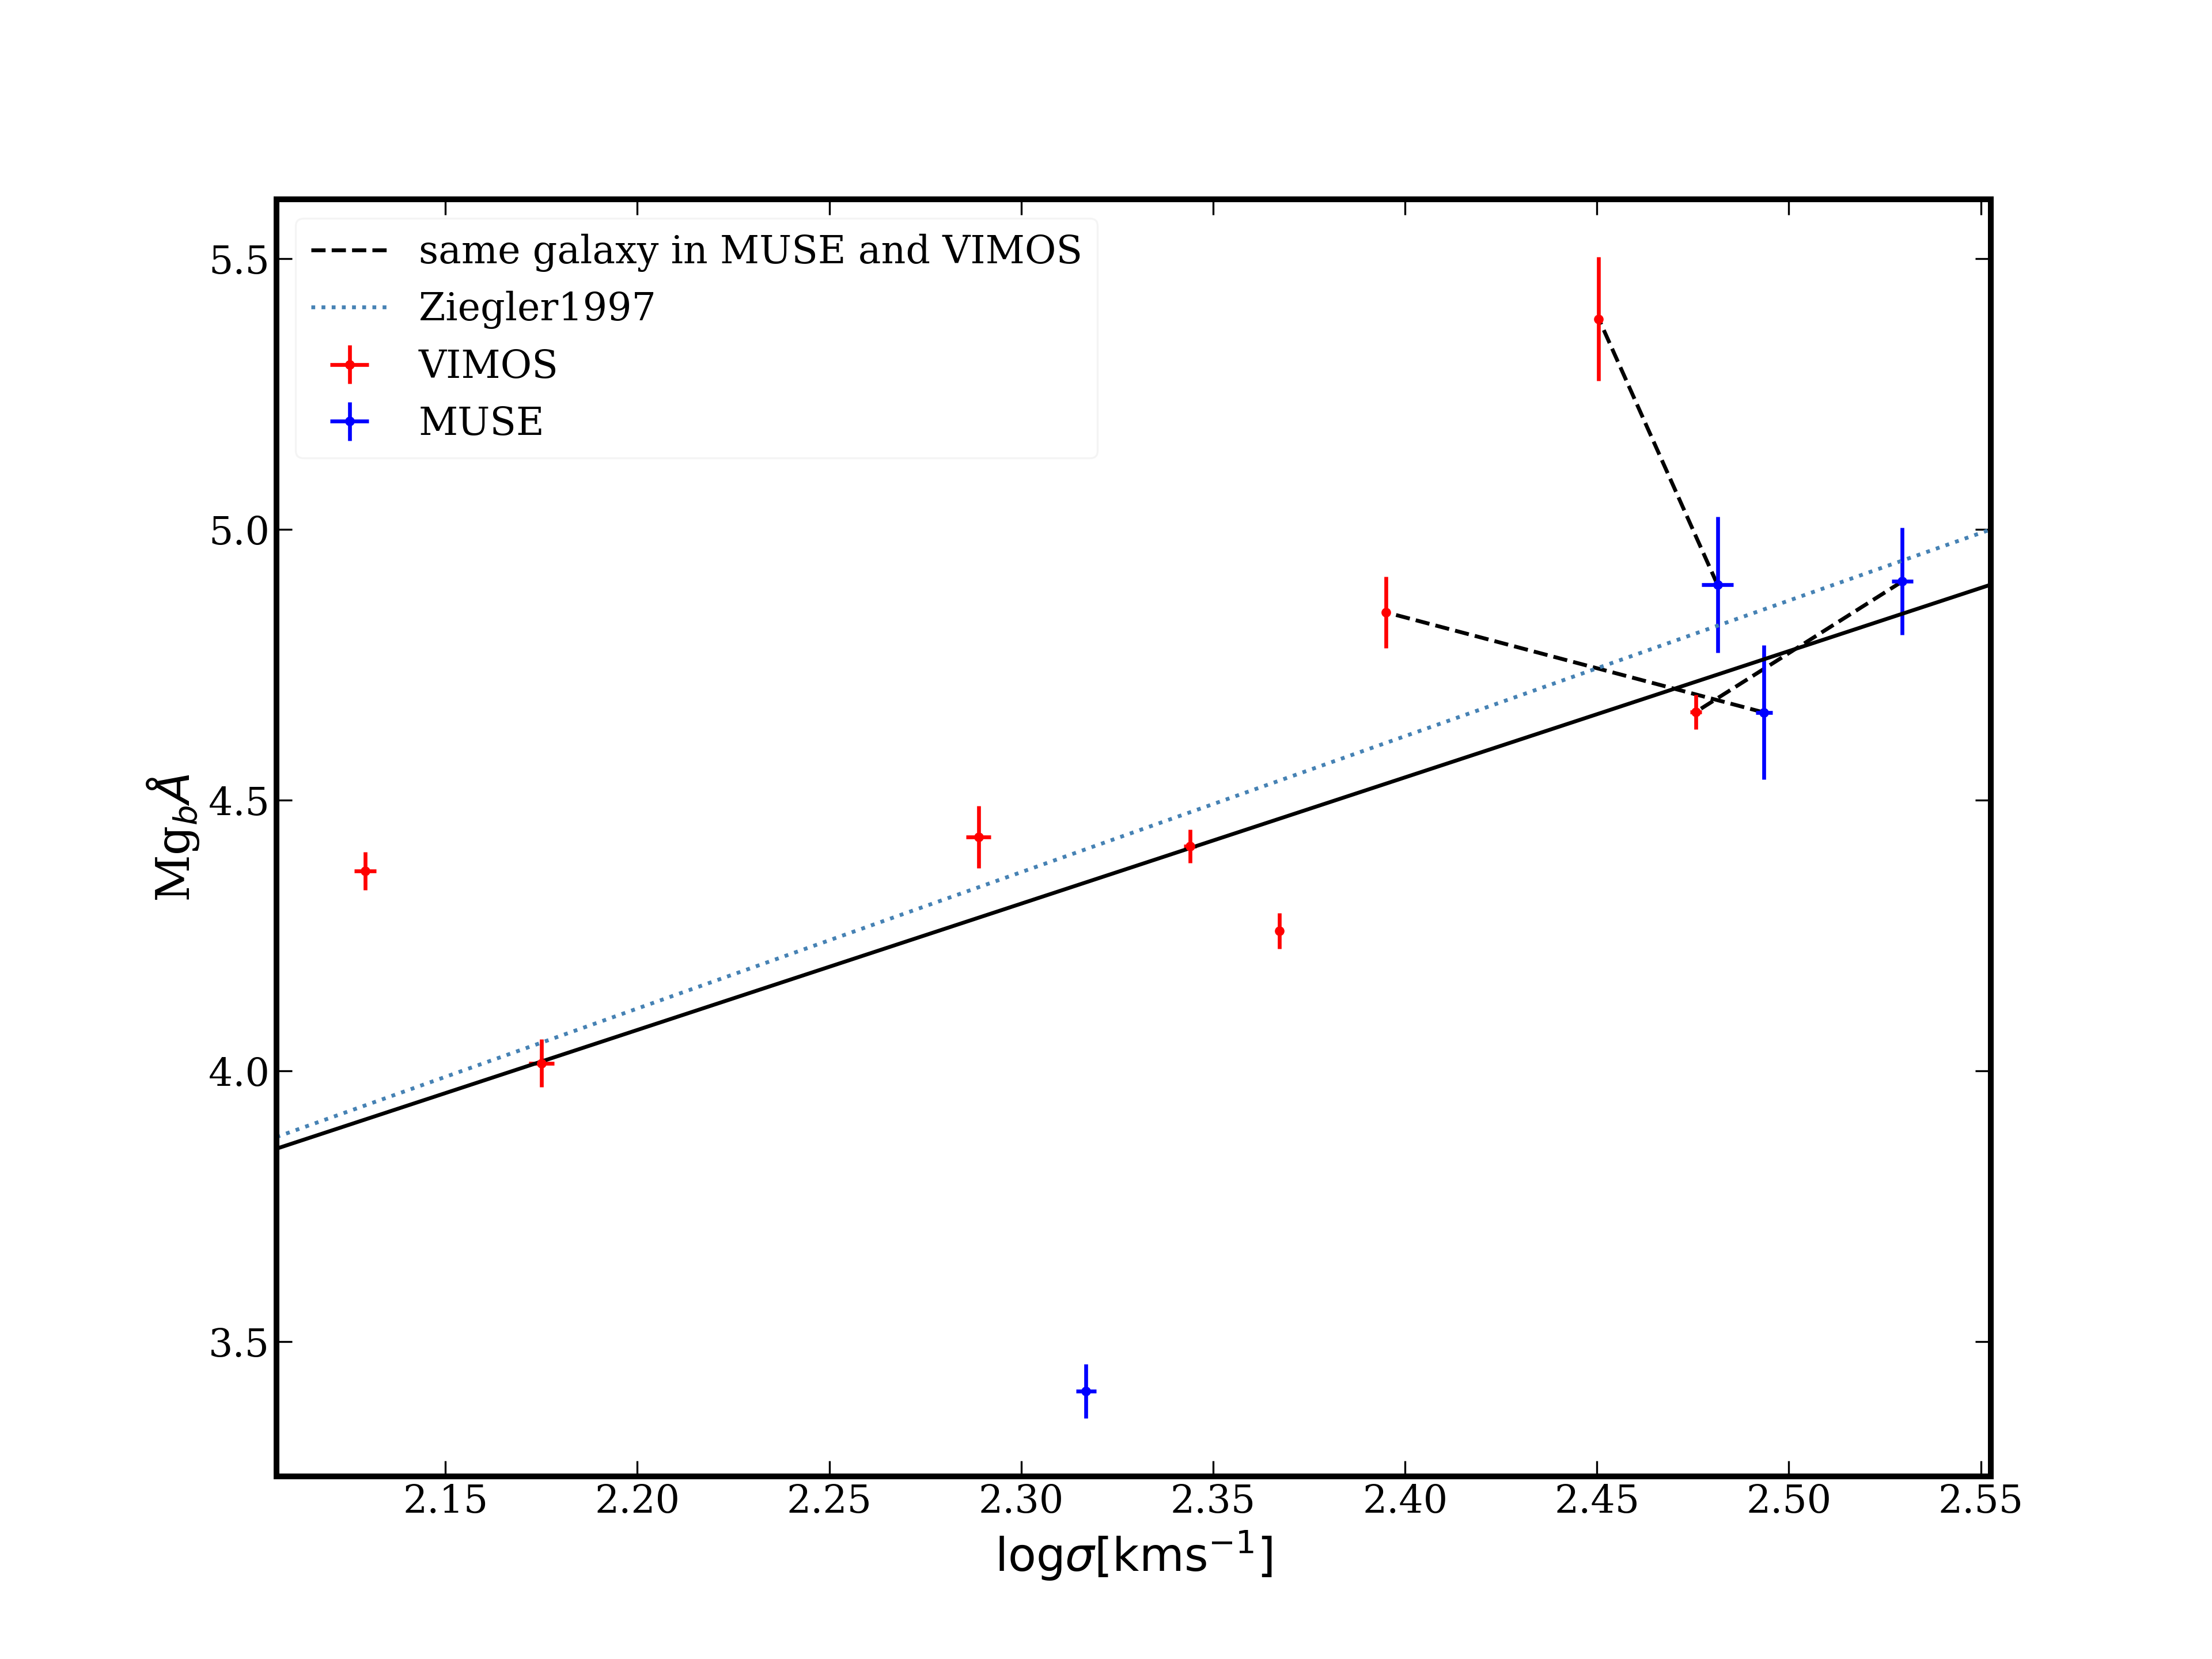
\includegraphics[width=.8\textwidth]{chapter4/Mg_sigma.png}
				\caption[Global Mg$_b$--$\sigma$]{The Mg$_b$ -- velocity dispersion relation using a 2" aperture. We find a similar gradient to our best-fitting line (solid) to that found by \citet{Ziegler1997} shown as the dashed lines, but with a significant offset.}
				\label{fig:globalMg}
			\end{figure}

		\subsubsection{Spatially Resolved}
			Since \citet{Mehlert2003} showed that the internal Mg -- $\sigma$ relation is entirely due to the metallicity and velocity dispersion radial gradients, we have not shown internal Mg -- $\sigma$ relationships as this adds no new information. Instead see section \ref{subsubsec:popGrad} for the radial gradients of the most-likely SSPs.

\section{The case of NGC 612}
	\label{sec:NGC612}
	All of the galaxies show typical ETG behavior: old, metal rich stellar populations with high stellar velocity dispersions with the exception of NGC 612. This galaxy has very high rotational velocities for an ETG, with an extended CO disc and a younger stellar population. All this suggests that NGC 612 may have a very different history to the rest of the Southern Sample. There are only a handful of known examples of disc-dominated radio galaxies \citep[e.g.][]{Morganti2011}. Spiral hosts are even rarer with only 4 known cases \citep{Ledlow1998, Hota2011a, Bagchi2014, Mao2015}.
